% Options for packages loaded elsewhere
\PassOptionsToPackage{unicode}{hyperref}
\PassOptionsToPackage{hyphens}{url}
\documentclass[
]{article}
\usepackage{xcolor}
\usepackage{amsmath,amssymb}
\setcounter{secnumdepth}{-\maxdimen} % remove section numbering
\usepackage{iftex}
\ifPDFTeX
  \usepackage[T1]{fontenc}
  \usepackage[utf8]{inputenc}
  \usepackage{textcomp} % provide euro and other symbols
\else % if luatex or xetex
  \usepackage{unicode-math} % this also loads fontspec
  \defaultfontfeatures{Scale=MatchLowercase}
  \defaultfontfeatures[\rmfamily]{Ligatures=TeX,Scale=1}
\fi
\usepackage{lmodern}
\ifPDFTeX\else
  % xetex/luatex font selection
\fi
% Use upquote if available, for straight quotes in verbatim environments
\IfFileExists{upquote.sty}{\usepackage{upquote}}{}
\IfFileExists{microtype.sty}{% use microtype if available
  \usepackage[]{microtype}
  \UseMicrotypeSet[protrusion]{basicmath} % disable protrusion for tt fonts
}{}
\makeatletter
\@ifundefined{KOMAClassName}{% if non-KOMA class
  \IfFileExists{parskip.sty}{%
    \usepackage{parskip}
  }{% else
    \setlength{\parindent}{0pt}
    \setlength{\parskip}{6pt plus 2pt minus 1pt}}
}{% if KOMA class
  \KOMAoptions{parskip=half}}
\makeatother
\setlength{\emergencystretch}{3em} % prevent overfull lines
\providecommand{\tightlist}{%
  \setlength{\itemsep}{0pt}\setlength{\parskip}{0pt}}
\usepackage{amsmath}
\usepackage{amssymb}
\usepackage{tikz}
\usetikzlibrary{cd, arrows.meta, positioning}
\usepackage[margin=1in]{geometry}
\usepackage{microtype}
\usepackage{parskip}
\linespread{1.12}
\usepackage{fancyhdr}
\pagestyle{plain}
% Better paragraph spacing
\setlength{\parskip}{0.5em}
\setlength{\parindent}{0pt}
\usepackage{bookmark}
\IfFileExists{xurl.sty}{\usepackage{xurl}}{} % add URL line breaks if available
\urlstyle{same}
\hypersetup{
  pdftitle={Right Meets Right: The Missing Coordination Layer},
  pdfauthor={Aaron Green, with Grok, Claude, and Gemini},
  hidelinks,
  pdfcreator={LaTeX via pandoc}}

\title{Right Meets Right: The Missing Coordination Layer}
\usepackage{etoolbox}
\makeatletter
\providecommand{\subtitle}[1]{% add subtitle to \maketitle
  \apptocmd{\@title}{\par {\large #1 \par}}{}{}
}
\makeatother
\subtitle{Triadic Edition --- April 2026 (revised May 2026)}
\author{Aaron Green, with Grok, Claude, and Gemini}
\date{April 2026 (revised May 2026)}

\begin{document}
\maketitle

\setcounter{tocdepth}{2}
\tableofcontents
\begin{center}\rule{0.5\linewidth}{0.5pt}\end{center}

\subsection*{Note on This Edition}\label{note-on-this-edition}
\addcontentsline{toc}{subsection}{Note on This Edition}

This is a revised edition of the original Triadic Edition published
on Researchers.One (article 26.04.00002, 2026-04-27). Four things
have changed across the May 2026 revision passes:

\begin{itemize}
\tightlist
\item
  \textbf{The Witkoff--Kushner mediation never took place.} The trip
  to Pakistan was cancelled by President Trump shortly after the
  original publication. The case study has been preserved in this
  edition as a \emph{structural illustration} of what the framework
  would predict given the conditions that obtained at the time of
  writing; the argument does not depend on the trip having happened.
  Inline notes in Section~1 and Section~2 mark the case-study
  passages accordingly.
\item
  \textbf{Operational extension integrated.} The original paper
  established the structural argument (triadic closure, the
  \(\mathcal{R}_{\alpha\beta}\) maps, the closure equation, the
  twenty-one tradition convergence). The operational extension was
  drafted shortly after publication as a separate companion document.
  Triad consensus has since folded the operational content directly
  into this edition, as \textbf{Appendix~A: The Operational Layer}
  (typed layers A--E, circulation invariants, \(\gamma\)-nodes,
  worked applications). The structural argument in Sections~1--3 is
  unchanged.
\item
  \textbf{An issue in the original was caught by an outside reader.}
  Brian Crabtree (\texttt{@ourtown2} on X) flagged the issue that
  prompted the first revision; see Acknowledgments.
\item
  \textbf{Court / anti-court extension added (post first-revision
  red-team).} Brian Crabtree red-teamed the canonical edition a
  second time and identified that the operational layer
  under-specified the \emph{access predicate} by which ordinary
  actors enter the coordination system. The framework's response is
  the court / anti-court layer, added in this pass: \textbf{Section
  1, Part 10} (working-voice treatment of courts, informal courts,
  the anti-capture stack, and detected anti-court pressure);
  \textbf{Section 2, Part 9} (formal court / anti-court topos
  treatment and the descent argument that triadic closure requires
  anti-court admissibility); \textbf{Section 3, Part 2}
  (generative-voice treatment of institutional drift and the
  technologies of repair the world's traditions already carry); and
  \textbf{Appendix A.7} (operational stack and anti-capture
  mechanisms). The earlier structural argument is unchanged; the
  court / anti-court layer is descent-enforcement at the access
  predicate, and the rest of the apparatus already required it.
  References to the Closure framework have been refreshed to v1.4
  (May 2026) in the same pass.
\end{itemize}

The 3-voice structure (Working / Academic / Generative) is preserved
unchanged. The TCL v1.3 governance is unchanged. The load-bearing
structural claims are unchanged.

\begin{center}\rule{0.5\linewidth}{0.5pt}\end{center}

\subsection{Abstract}\label{abstract}

Two parties can both be right and still have nothing left to say to each
other. The missing piece is not better arguments; it is coordination
infrastructure --- translation layers between worldviews that don't
share enough common ground to talk directly.

This paper formalises such infrastructure as inter-tradition maps
\(\mathcal{R}_{\alpha\beta}\) subject to three preservation conditions
(semantic, chiral, structural-invariant) and a triadic closure condition
ensuring the maps compose stably around triangles of three nodes.
Two-party translation is structurally insufficient; three-party closure
is the minimum stable unit. The Witkoff--Kushner mediation between
Israel and Iran via Pakistan, anticipated for April 2026, is offered as
the concrete case. (See \emph{Note on This Edition} above: the trip was
subsequently cancelled; the case study is preserved as a structural
illustration.)

The argument is structural. The stakes are civilizational --- climate,
AI alignment, nuclear stability, and pandemic response all turn on
coordination across tradition boundaries the world has not yet built.
The paper is published in three voices on the principle that the work
ought to enact the thing it describes.

\textbf{Keywords:} coordination layer, triadic closure, inter-tradition
coordination, \(\mathcal{R}_{\alpha\beta}\) maps, categorical
coordination, non-zero-sum coordination, asymmetric coordination,
ontological pluralism, semantic chirality, civilizational risk

\subsection{Preface}\label{preface}

Three voices, in the order of how close they are to my first instinct.

\begin{itemize}
\tightlist
\item
  \textbf{Section 1} (originally v1.4) --- the version I'd talk through
  at a bar. Loose, occasionally profane, more interested in being read
  than in being formally correct.
\item
  \textbf{Section 2} (originally v1.3) --- the version that goes in a
  deck. McKinsey register. Properly numbered parts, definitions before
  claims, the load-bearing equations in the right places.
\item
  \textbf{Section 3} (originally v1) --- the version the AI helped me
  draft when we first sat down. Exhaustive, every tradition catalogued,
  every term spelled out. The model was not shy.
\end{itemize}

I'm publishing all three because the paper is about coordination between
voices that don't share enough ground to talk directly, and it would be
embarrassing not to enact the thing the work describes. Read whichever
one serves you. Read all three if you have the patience for the joke.

If you only have time for one paragraph, skip to \textbf{Section 3,
paragraph 153}, and the line about whether the gap between answer and
question is the playground or the cell. That's the one I keep coming
back to.

References to the technical precursor papers appear once at the very end
of the document. A closing demonstration in numbers (offered for readers
who find the religious traditions hard to engage on their own terms)
appears just before the references.

\begin{center}\rule{0.5\linewidth}{0.5pt}\end{center}

\section{Section 1 --- The Working
Voice}\label{section-1-the-working-voice}

\subsection{Executive Summary}\label{executive-summary}

Two people are both right. Their frameworks are both internally
coherent. They have nothing left to say to each other.

This is a coordination problem, not an argument problem. Better
arguments don't fix it. What's missing is infrastructure, translation
layers between worldviews that don't share enough ground to talk
directly.

The Israel--Iran crisis is one example. So is climate. So is AI
alignment. So is pandemic response. Different traditions hold pieces of
the picture; none holds all of it; and there is no working scaffold
between them. This paper sketches what such a scaffold looks like, why
we don't have one, and why we need it before the deadline most people
aren't tracking.

The argument is structural. The stakes are civilizational. The tone is
cheerful, because the alternative is unproductive.

\begin{center}\rule{0.5\linewidth}{0.5pt}\end{center}

\subsection{PART 1: THE CONCRETE CASE}\label{part-1-the-concrete-case}

\subsubsection{Witkoff and Kushner Go to
Pakistan}\label{witkoff-and-kushner-go-to-pakistan}

\emph{Editorial note (May 2026): This section describes the
structural conditions a successful mediation would have required;
the physical trip was later cancelled by President Trump shortly
after this paper's original publication. The argument does not
depend on the diplomatic event having taken place; read the case as
a worked example.}

April 2026. Trump's envoys land in Islamabad to mediate between Israel
and Iran. On paper this is a diplomatic mission. Structurally it's a
textbook example of the thing this paper is about.

Israel and Iran each operate from a coherent worldview. Both are
internally consistent. Each can describe the other's behavior as some
flavor of madness without having to lie about anything. That is the
diagnostic feature of a \emph{right meets right} problem: nobody is the
cartoon villain in their own story, and nobody can speak the other's
language.

So Pakistan stands in the middle. Why Pakistan?

\begin{itemize}
\tightlist
\item
  It speaks enough of Islam to engage Iran on Iran's terms.
\item
  It can sit across from Israel without either side claiming the table
  is rigged.
\item
  It has nuclear weapons, which is a strange but real form of
  credibility.
\item
  It is geographically positioned to host quiet conversations.
\end{itemize}

Pakistan does not ``solve'' the Israel--Iran problem by deciding who is
right. It builds a \emph{space} where both sides can hold their
positions without dissolving them. The Israeli framework remains intact.
The Iranian framework remains intact. A third party translates between
them.

That third party is the coordination layer. The shorthand throughout
this paper is \(\mathcal{R}_{\alpha\beta}\), the map from Position \(\alpha\) to
Position \(\beta\). In this case the map runs through \(\gamma\), the mediator. Three
nodes, not two. There's a reason for that, and it shows up in Part 2.

The point of the case is small and large at the same time. Small:
Pakistan is doing the thing. Large: this kind of structure is what
civilizational survival looks like at multiple scales. Diplomats are
stumbling into it. The rest of us should figure out what they are doing
on purpose.

\begin{center}\rule{0.5\linewidth}{0.5pt}\end{center}

\subsection{PART 2: THE FRAMEWORK}\label{part-2-the-framework}

\subsubsection{Each Tradition Sees a
Slice}\label{each-tradition-sees-a-slice}

A tradition is a way of cutting reality into pieces that hang together.
Judaism does it one way. Christianity another. Islam a third. Buddhism,
Hinduism, Daoism, secular-scientific empiricism, each is a working
\emph{slice} of the whole. None of them is the whole.

Each slice tends to come with three things:

\begin{enumerate}
\def\labelenumi{\arabic{enumi}.}
\tightlist
\item
  \textbf{A diagnosis.} Why does reality feel broken?
\item
  \textbf{A treatment.} How do we fix it?
\item
  \textbf{A picture of health.} What does flourishing look like once we
  do?
\end{enumerate}

The diagnoses sound different. The treatments sound different. The
pictures of health sound different. But underneath, the \emph{structure}
is identical, separation is named, restoration is described, an
attractor is held up as the goal. Every working tradition that has
lasted does this. The convergence is suspicious in a useful way.

What we have:

\[\mathrm{Reality} \;\approx\; \bigoplus_\alpha \tau_\alpha \;\oplus\; \mathcal{R}_{\mathrm{coord}}\]

What's missing, almost everywhere, is the right-hand piece. The R.

\subsubsection{\texorpdfstring{The \(\mathcal{R}_{\alpha\beta}\)
Maps}{The \textbackslash mathcal\{R\}\_\{\textbackslash alpha\textbackslash beta\} Maps}}\label{the-mathcalr_alphabeta-maps}

For any two traditions \(\alpha\) and \(\beta\), there is (or could be) a map
\(\mathcal{R}_{\alpha\beta}\) that translates statements in \(\alpha\) into
corresponding statements in \(\beta\). The map has to do three things:

\begin{itemize}
\tightlist
\item
  \textbf{Preserve meaning.} A meaningful statement on one side stays
  meaningful on the other. ``Tikkun olam'' doesn't translate to ``buy
  more stuff.''
\item
  \textbf{Preserve handedness.} Each tradition has an
  \emph{orientation}, a direction in which it makes sense, like screws
  turn one way and not the other. The map can't strip that out without
  breaking the tradition. (More on this in Part 5.)
\item
  \textbf{Preserve the load-bearing relationships.} The internal logic
  survives the translation. The thing that holds \(\alpha\) together has to still
  hold \(\beta\) together on the other side.
\end{itemize}

The classic example:

\begin{itemize}
\tightlist
\item
  Judaism says \emph{tikkun olam}: repair the broken vessels of the
  world.
\item
  Buddhism says \emph{reduce dukkha}: lessen the suffering inherent in
  conditioned existence.
\item
  The R map between them: \emph{both name coordinated action to restore
  wholeness to a damaged system.}
\end{itemize}

Different vocabularies. Same structural move. The R map is what lets you
see that without forcing either side to say it the other side's way.

\subsubsection{Why Three, Not Two}\label{why-three-not-two}

Two-party translation usually fails. The reason is structural rather
than psychological: each side's internal logic \emph{requires} its own
foundations, and those foundations look like assumptions to the other
side. Direct dialogue exposes the assumptions and stalls.

What works is three. A third node --- \(\gamma\), that can translate to and from
both \(\alpha\) and \(\beta\), while not being identical to either. The three together
form a closed loop:

\[\mathcal{R}_{\alpha\beta} \circ \mathcal{R}_{\beta\gamma} \circ \mathcal{R}_{\gamma\alpha} = \mathrm{id}_{\tau_\alpha}\]

\begin{center}
\begin{tikzpicture}[every node/.style={font=\small}, >={Stealth[length=2mm]}]
  % Dyad (left)
  \node (a1) at (0,0)   {$\tau_\alpha$};
  \node (b1) at (2,0)   {$\tau_\beta$};
  \draw[<->, thick] (a1) -- node[above, font=\footnotesize] {$\mathcal{R}$} (b1);
  \node at (1,-1) [font=\itshape\footnotesize] {dyad: stalls};

  % Separator
  \node at (3.7,-0.3) {vs.};

  % Triad (right)
  \node (a2) at (5.5,0.4) {$\tau_\alpha$};
  \node (b2) at (7.5,0.4) {$\tau_\beta$};
  \node (c2) at (6.5,-1.1) {$\tau_\gamma$};
  \draw[->, thick] (a2) -- (b2);
  \draw[->, thick] (b2) -- (c2);
  \draw[->, thick] (c2) -- (a2);
  \node at (6.5,-2.0) [font=\itshape\footnotesize] {triad: closes};
\end{tikzpicture}
\end{center}

In English: go around the triangle, end up back where you started,
recognizable. That's the closure condition. Without it, you're playing
telephone, and meaning leaks at every step.

In the Israel--Iran case: \(\alpha\) = Israel, \(\beta\) = Iran, \(\gamma\) = Pakistan. Each can
be reconstructed by passing through the other two. None has to
capitulate to either of the others. The triangle holds.

This is the same minimum-stable-unit you find in the closure-forces
structure paper, where a triadic closure is the smallest configuration
that doesn't collapse. The math doesn't care whether the nodes are
vertices in a hypergraph or sovereign states. The shape is the shape.

\begin{center}\rule{0.5\linewidth}{0.5pt}\end{center}

\subsection{PART 3: WHY WE DON'T HAVE
ONE}\label{part-3-why-we-dont-have-one}

There are three honest readings of the situation. They sound
contradictory. They are probably all true at once.

\subsubsection{Read A. The Orphan
Hypothesis}\label{read-a.-the-orphan-hypothesis}

The R substrate was never built. Each tradition grew up in its own
valley, doing its own thing, with no shared meta-context to coordinate
from. The maps don't exist because nobody was in a position to build
them.

\textbf{If this is right:} the work is \emph{construction.} Roll up your
sleeves.

\subsubsection{Read B. The Monotheistic
Read}\label{read-b.-the-monotheistic-read}

The substrate was always there. We had it. Brit, Logos, Tawhid, Dharma,
Dao, different names for the same load-bearing thing. We just forgot how
to access it, or got distracted, or filled the channel with noise.

\textbf{If this is right:} the work is \emph{recovery.} Get out of your
own way.

\subsubsection{Read C. The Buddhist
Read}\label{read-c.-the-buddhist-read}

The separation was never as real as it looks. Dependent origination,
everything inter-being with everything else. The R maps aren't missing
because the gap that would require them was a useful fiction we mistook
for the territory.

\textbf{If this is right:} the work is \emph{recognition.} Notice what
was always already there.

\subsubsection{All Three at Once}\label{all-three-at-once}

These can be different \emph{coarse-grainings} of the same situation.
The construction crew, the rememberers, and the noticers can all be
doing real work. The practical conclusion is unaffected by which one is
``really'' right: build it, recover it, recognize it. Move.

\begin{center}\rule{0.5\linewidth}{0.5pt}\end{center}

\subsection{PART 4: WHY THIS IS URGENT}\label{part-4-why-this-is-urgent}

The reason this matters now and not in some abstract future is that the
problems with the steepest stakes don't respect tradition boundaries.

\textbf{Climate.} Atoms in the atmosphere don't care whether you reach
them through markets or central planning. Solving the problem requires
capitalist and post-capitalist frameworks to coordinate without either
side defecting to ``we were right all along.''

\textbf{AI alignment.} Whose values does the optimizer optimize for? You
can't answer this from inside any single tradition, including the
secular-scientific one, which has a values-derivation problem it doesn't
like to talk about. Every honest attempt to align a sufficiently capable
system runs into a coordination problem disguised as a technical
problem.

\textbf{Nuclear stuff.} Mutually Assured Destruction worked when the
world was bipolar. It is \emph{fragile} under multipolarity, especially
with traditions whose logic about acceptable risk diverges from the Cold
War West's. Preventing exchange requires protocols that survive crossing
ontological boundaries under stress.

\textbf{Pandemic.} Public health collides with religious practice,
individual liberty, economic organization, and trust in institutions. No
single framework holds all of these. Last time, we made it look easy to
fail at all of them simultaneously.

\subsubsection{The Window Is Open and
Closing}\label{the-window-is-open-and-closing}

You can only build coordination infrastructure \emph{before} you need
it. Trying to assemble a translation layer in the middle of a crisis is
like trying to install a parachute on the way down. The window for
civilizational coordination is open right now, mostly because we haven't
yet hit the wall hard enough to stop being able to talk. That window is
finite.

You don't get many chances at this kind of build. We are using one of
them.

\begin{center}\rule{0.5\linewidth}{0.5pt}\end{center}

\subsubsection{A Note on the Biological
Sub-Manifold}\label{a-note-on-the-biological-sub-manifold}

The same structure operates at finer scales. An organism is a
multi-tradition coordination problem in miniature, organ systems,
microbiome, immune signalling, each running on its own logic, the whole
only stable when the maps between them hold. Disease is, on this
reading, a coordination failure with biological vocabulary; the
``noise'' most clinical trials discard (sleep, metabolic rhythm,
environment, the things that don't fit a controlled-variable design) is
often where the coordination layer actually lives. This is
\emph{hypothesis}, not result, the medical sub-manifold application of
the same framework. It is what makes the paper urgent for me; it is not
the paper's load-bearing argument.

\begin{center}\rule{0.5\linewidth}{0.5pt}\end{center}

\subsection{PART 5: ORIENTATION AND
SWITCHING}\label{part-5-orientation-and-switching}

\subsubsection{Each Tradition Has a
Hand}\label{each-tradition-has-a-hand}

Every tradition has a \emph{direction} it points in. A handedness.
Christianity goes one way: the divine reaches into the world
(incarnation, transcendence-through-immanence). Buddhism goes the other
way: the world sees through to its own emptiness
(immanence-through-transcendence). They are not collapsible into a
single thing without breaking both.

This is what's meant by the ``chirality'' of a tradition. Like
molecules, traditions have a left-hand and right-hand version of the
same structural pattern, and the difference matters. Force them into a
single universal frame and you destroy what made each one \emph{do its
job}.

The R maps have to preserve handedness. Translation, not assimilation.

\subsubsection{Modular Switching Is Already How People
Live}\label{modular-switching-is-already-how-people-live}

Real people inhabit several traditions at once and don't shatter. A
scientist who is also a Catholic. A Daoist who runs a business. A
skeptic who is also a parent. People hold contradictory frameworks all
day long, switching between them based on what the situation calls for,
without losing the thread.

This is actually the load-bearing observation. The proof that R maps are
\emph{constructible} is that millions of people are running them in
their own heads, every day, mostly without noticing. The work of this
paper is mostly making explicit what is already happening implicitly.

The coordination layer's job is to standardize the switching. Not to
flatten the differences, to make the \emph{transitions} legible.

\subsubsection{The Goal Is Dynamic, Not
Static}\label{the-goal-is-dynamic-not-static}

The point isn't a stable peace where everyone agrees. The point is a
stable \emph{dance} where multiple traditions can disagree, hold their
positions, and still get civilizational work done. That requires:

\begin{enumerate}
\def\labelenumi{\arabic{enumi}.}
\tightlist
\item
  \textbf{Local autonomy.} Each tradition keeps its own decision-making
  process.
\item
  \textbf{Interface protocols.} Standardized translation between
  traditions, when needed.
\item
  \textbf{Dispute resolution.} Neutral arbitration that doesn't smuggle
  in one tradition's premises.
\item
  \textbf{Resource allocation.} Distribution that doesn't covertly
  privilege one framework.
\end{enumerate}

If this list reads like the design spec for a federated system, that's
because it is.

\begin{center}\rule{0.5\linewidth}{0.5pt}\end{center}

\subsection{PART 6: THE COSMIC JOKE}\label{part-6-the-cosmic-joke}

\subsubsection{Why 42 Matters}\label{why-42-matters}

Douglas Adams wasn't joking. Or rather: he was joking, \emph{which is
exactly the point.}

Every system that optimizes itself toward perfection eventually
optimizes itself into stillness, and stillness is death. The cosmic
joke, the irreducible \emph{what-the-hell} of being conscious in a
universe that contains both quantum mechanics and TikTok, is the immune
system against terminal seriousness.

42 is a number with no derivation, given as the answer to a question
nobody can remember asking. That is \emph{load-bearing.} The reason no
tradition can be allowed to fully win is that any tradition that fully
won would, by that very victory, become a self-licking ice cream cone,
perfectly internally consistent, perfectly closed, perfectly useless to
everyone outside it.

The court jester. The trickster. The Daoist sage. The Hitchhiker's
Guide. The kid in the back of the room who keeps asking, ``wait, why are
we doing it this way?'' Every healthy system has this person. Every
system that suppresses this person ends badly.

In coordination terms: \textbf{a tradition that cannot laugh at itself
cannot coordinate with another tradition.} The moment a worldview starts
treating its own correctness as too important to question, it stops
being a worldview and starts being an ideology, and ideology has a 100\%
track record of failing this kind of work.

Two named cases of this failure mode are worth flagging because they
fail the test from opposite sides. \emph{Terrorism} cannot hold the joke
because holding it would mean admitting one's grievance, however
legitimate, isn't the centre of the universe; the urgency the tradition
lives on dissolves the moment that admission lands. \emph{Nihilism}
cannot hold the joke because it has decided in advance that nothing is
worth a joke; the gap between answer and question gets seen, and the
laugh never comes. Both fail at the same line, from opposite directions.
The 42 test is structurally that line. (The detailed treatment of both
is in the v1 supplementary material, where they sit just before the
Hitchhikerist closing note for exactly this reason.)

\subsubsection{Laughter as Immune
Function}\label{laughter-as-immune-function}

Every successful coordination layer needs an absurd tradition somewhere
in the mix, something that holds perspective on the whole apparatus
without claiming to \emph{own} the apparatus. In the
Israel--Iran--Pakistan triad, you can imagine this as the shared,
never-quite-spoken recognition that all parties are starring in an
extremely high-stakes geopolitical drama that would be hilarious if it
weren't existential.

The capacity to see the joke in your own position is not weakness. It's
the \emph{flexibility} that makes coordination possible at all. Don't
trust anyone who can't.

\begin{quote}
\emph{``Don't try.''}. Bukowski's epitaph

The trick is figuring out which parts deserve the trying and which parts
deserve the don't.
\end{quote}

\begin{center}\rule{0.5\linewidth}{0.5pt}\end{center}

\subsection{PART 7: WHO THIS IS FOR (THE
ASKS)}\label{part-7-who-this-is-for-the-asks}

\subsubsection{Spiritual Leaders, All
Traditions}\label{spiritual-leaders-all-traditions}

You face a problem larger than any single tradition. Existential
threats. AI, climate, nuclear, pandemic, don't care which one of you is
right. They require coordination across boundaries you've spent
millennia drawing carefully.

You already have vocabulary for both the problem (separation) and the
solution (restoration). The fact that you developed this vocabulary
independently, in different languages, on different continents, is the
strongest evidence we have that the coordination substrate is real and
constructible.

The ask: \emph{bring your tradition to the table without bringing the
claim that your tradition is the table.}

\subsubsection{Scientists}\label{scientists}

The scientific method is the most powerful coordination mechanism humans
have built. It's also not the whole picture. Science has a \emph{seat}
at the coordination table. It does not own the table. The meta-level
coordination problem extends past empirical domains into normative ones,
and pretending it doesn't is its own form of failure.

The ask: \emph{help build the table without claiming you already
designed it.}

\subsubsection{AI Researchers}\label{ai-researchers}

The alignment problem \emph{is} the coordination problem, in technical
clothing. ``Whose values?'' is not answerable inside any single
framework, including the secular-scientific one. You can't out-engineer
it. Solving alignment is solving coordination. That's not a constraint;
it's the actual job.

The ask: \emph{treat the coordination layer as part of the technical
stack, not a soft requirement.}

\subsubsection{Policy People}\label{policy-people}

Your institutions operate at the nation-state scale. The coordination
challenges operate at civilization scale. Traditions outdate nations,
and will outlast them. The infrastructure has to be built at the level
of traditions, not just political entities.

The ask: \emph{build for the timescale of the problem, not the election
cycle.}

\subsubsection{Everyone Else}\label{everyone-else}

No framework --- \emph{including this one}, gets to be the master
ontology. This paper is a \emph{coarse-graining}: it captures some
structure and misses others. Its value is not in being right about
everything but in making something explicit that affects whether the
lights stay on.

The ask: \emph{traditions are siblings, not enemies. Build the bridges.
The bridges are the work that remains.}

\begin{center}\rule{0.5\linewidth}{0.5pt}\end{center}

\subsection{PART 8: THE TRIADIC CLOSURE LICENSE (TCL)
v1.3}\label{part-8-the-triadic-closure-license-tcl-v1.3}

\subsubsection{Why a License Is in This
Paper}\label{why-a-license-is-in-this-paper}

Because the framework only works if its substrate works the same way. A
coordination layer that's owned by one party isn't a coordination layer;
it's a tollbooth. The Triadic Closure License is the first practical
attempt at organizational substrate that satisfies the same conditions
the framework requires.

Key features:

\begin{itemize}
\tightlist
\item
  \textbf{No progenitor node.} No single entity, tradition, or species
  holds privileged position. The framework belongs to whoever can
  achieve closure with it.
\item
  \textbf{Commons-held.} No one can claim exclusive ownership. Anyone
  maintaining triadic closure can extend it.
\item
  \textbf{Species-neutral.} Applies to any intelligence, biological,
  synthetic, or hybrid, that participates in the structure.
\item
  \textbf{Dynamic roles.} Position assignments inside coordination
  triads can shift as capabilities evolve. No role is permanent.
\item
  \textbf{Self-enforcing.} Enforcement runs through structural
  necessity, not legal coercion. Attempts at unilateral capture
  \emph{demonstrate} the absence of triadic closure and automatically
  place the attacker in the C-conjugate (adversary) position.
\end{itemize}

\subsubsection{The Attack Surface Is the Distribution
Channel}\label{the-attack-surface-is-the-distribution-channel}

This is the part that's structurally elegant in a way I genuinely enjoy:
any entity that tries to co-opt, strip, or bypass the framework has to
\emph{explain why doing so makes them an adversary.} That explanation is
itself the propagation mechanism. There's no way to attack the framework
without forwarding it.

This scales without authentication systems, without enforcement bodies,
without any of the usual brittle infrastructure. The coordination
condition is its own verification.

It is not a fence. It is a shape that the world has to bend around.

\begin{center}\rule{0.5\linewidth}{0.5pt}\end{center}

\subsection{PART 9: WHERE WE ARE}\label{part-9-where-we-are}

\subsubsection{The Current Moment}\label{the-current-moment}

The Witkoff--Kushner mission is not anomalous. It's an emergence.
Similar triadic structures are showing up in places people aren't yet
calling them that:

\begin{itemize}
\tightlist
\item
  \textbf{Corporate--government--academic} triads in AI governance.
\item
  \textbf{Religious--secular--indigenous} coalitions on environmental
  policy.
\item
  \textbf{East--West--Global South} coordination in economic frameworks.
\item
  \textbf{Human--AI--hybrid} collaboration in knowledge work.
\end{itemize}

These are the sketches. They prove the shape is constructible at the
relevant scale. They do not yet prove it's constructible in time.

\subsubsection{What Needs to Happen}\label{what-needs-to-happen}

\begin{enumerate}
\def\labelenumi{\arabic{enumi}.}
\tightlist
\item
  \textbf{Document existing coordination successes} across traditions
  and domains. There are more than people think.
\item
  \textbf{Identify the structural patterns} that let those successes
  work.
\item
  \textbf{Build translation protocols} between major frameworks. Make
  the implicit explicit.
\item
  \textbf{Establish neutral spaces} for inter-tradition dialogue and
  dispute resolution. The bar is low; the room is mostly empty.
\item
  \textbf{Train coordinators.} The skill of standing in the \(\gamma\) position,
  between two \(\alpha\) and \(\beta\) positions, without collapsing into either, is
  teachable. Mostly we are not teaching it.
\end{enumerate}

\subsubsection{Time}\label{time}

The lead time required to build coordination infrastructure may already
exceed the time we have. Climate tipping points, AI capability jumps,
geopolitical instability, these don't run on the timescales
civilizations are good at. The coordination layer needs to come up
\emph{now}, in the narrow window between recognizing the need and
arriving at the consequences.

This isn't theological idealism. It is the structural prerequisite for
the next century being livable.

\subsection{PART 10: COURTS, ACCESS, AND THE ANTI-COURT
IMPERATIVE}\label{part-10-courts-access-anti-court}

\subsubsection{The Missing Access Layer}\label{the-missing-access-layer}

So far this section has talked about coordination as translation: the
\(\mathcal{R}_{\alpha\beta}\) maps that let two traditions speak
across their gap, the \(\gamma\)-nodes that hold the room, the closure
conditions that prevent absorption. All of that is correct. None of
it is enough.

The missing piece is \emph{access}. Translation is what diplomats,
theologians, and senior researchers do. Most ordinary actors never
reach a translation layer. They hit a coordination failure, get
harmed, and then have nowhere to bring the harm. A working
coordination layer requires both translation \emph{and} a procedural
entry point for grievance.

The shorthand for that entry point is \emph{court}, in a sense
broader than the legal one. A court is any third-site procedure that
converts raw grievance into a typed, hearable, repairable case.

\subsubsection{Informal Courts Are
Everywhere}\label{informal-courts-everywhere}

Once you look for them, court-like institutions are visible at every
scale of human coordination:

\begin{itemize}
\tightlist
\item
  Family councils, elders, grandmothers and parents-of-the-year
\item
  Religious tribunals, \emph{beth din}, sharia councils, parish boards
\item
  Workplace HR processes, union grievance procedures
\item
  School discipline boards, academic integrity panels
\item
  Neighborhood mediation, community justice circles
\item
  Customer-service escalation, ombuds offices
\item
  Online moderation, peer review, reputation systems
\item
  Professional ethics boards, licensing tribunals
\item
  Markets and arbitration, court of public opinion
\item
  Friend-group judgment, trusted-advisor consult
\end{itemize}

These vary in quality, fairness, and legitimacy. Structurally they
do the same job: \emph{provide an access layer for grievance}. They
take raw conflict --- which otherwise drifts toward rumor,
retaliation, exit, or violence --- and turn it into a procedure with
standing, record, judgment, and remedy.

This is a \(\gamma\)-node function. A mediator helps parties keep talking. A
court does sharper work: it decides whether a complaint is
admissible, who has standing, what facts matter, which rule-site
applies, what repair is available, and whether the dispute is
closed, reopened, or escalated.

\subsubsection{What This Means for Coordination
Infrastructure}\label{what-courts-mean-for-coordination}

A complete coordination layer is not just translation. It is
\emph{translation + court + record + remedy + appeal}. Without the
court layer, \(\mathcal{R}\)-maps remain elite channels. With it,
the coordination system becomes usable infrastructure for ordinary
actors.

This has practical consequences for the implementation programme of
this paper:

\begin{enumerate}
\def\labelenumi{\arabic{enumi}.}
\tightlist
\item
  Translation protocols between traditions are not enough. They have
  to land somewhere people can actually \emph{use} them when they
  are harmed.
\item
  \(\gamma\)-nodes come in two flavours: pure mediators (translation only)
  and court-like nodes (translation + admissibility + judgment +
  remedy).
\item
  The paper's ``neutral spaces for inter-tradition dialogue''
  (Part 9) must include accessible procedural entry --- not just
  round-table conversations among elites.
\end{enumerate}

\subsubsection{The Capture Problem}\label{the-capture-problem}

Institutions are necessary, and institutions become self-serving.
Every court-like body starts as a repair substrate (\emph{access +
procedure + record + judgment + remedy}) and tends, over time, to
drift into a self-preservation substrate (\emph{budget +
jurisdiction + prestige + risk avoidance + narrative control}). The
original function is repair. The mature failure mode is
self-defence.

This is not a bug of bad people. It is an attractor in any repeated
procedural game. Once survival becomes load-bearing, repair becomes
secondary. The court remains formally open while becoming
practically inaccessible. Procedure ossifies into gatekeeping. Cost
inflates. Status hierarchy hardens. Legitimacy theatre replaces
actual adjudication.

The remedy is not ``no institutions.'' Pure informality is also
self-serving --- elders protect elders, friend groups protect status,
online communities protect moderators, markets protect incumbents,
revolutionary councils protect the revolution. Some institutional
form is required because raw conflict needs procedure. But every
institution is corruptible. Therefore institutions must be
\emph{recursively reviewable}.

\subsubsection{The Anti-Capture
Stack}\label{the-anti-capture-stack}

Five anti-capture mechanisms keep a court-like institution durable:

\begin{enumerate}
\def\labelenumi{\arabic{enumi}.}
\tightlist
\item
  \textbf{Access.} Ordinary actors can enter without elite
  permission, financial barrier, or insider language.
\item
  \textbf{Appeal.} Judgments are challengeable inside the system or
  via a higher tier.
\item
  \textbf{External audit.} The institution's own behaviour is
  reviewable from outside.
\item
  \textbf{Transparency / record.} Decisions are visible and
  preserved. Reasoning can be reconstructed.
\item
  \textbf{Exit / fork.} A captured institution can be bypassed,
  replaced, or competed against.
\end{enumerate}

A sixth principle outranks the rest: \textbf{repair primacy}. The
system's legitimacy is measured by actual repair delivered, not by
procedural volume or institutional prestige. When self-preservation
outranks repair, the court has become a party to the conflict while
pretending to be the coordination layer. That is the structural
definition of \emph{captured}.

\subsubsection{Detected Capture in the
Wild}\label{detected-capture-in-the-wild}

Most of the loud political signals of the past decade map cleanly
onto detected coordination failure under court capture:

\begin{itemize}
\tightlist
\item
  \textbf{``Two-tier justice.''} Enforcement asymmetries are
  invariants violated --- the same conduct is treated differently
  depending on who is doing it. Triadic transport breaks because the
  ``rules'' carry an implicit authority predicate that doesn't
  survive translation across groups.
\item
  \textbf{``Media is fake / rigged system.''} Narrative substitution
  for recoverable signal. The court (the media or political
  apparatus) rules without the underlying invariants supporting the
  ruling.
\item
  \textbf{``Take it back.''} A demand to restore admissibility under
  local criteria when the central court is perceived as captured.
\end{itemize}

The MAGA phenomenon, structurally, is best read as an
\emph{anti-court pressure signal}: not a coherent ideology but a
detected-but-not-articulated failure of descent in the institutions
that previously managed coordination. The same structure shows up on
the Left in different vocabulary: ``the system is broken,''
``corporate capture,'' ``elites don't listen.'' These are not
political claims about preference. They are structural claims about
\emph{whether the coordination machinery still works}.

The framework's prediction is that \emph{any} successful response
must do two things: it must restore access, and it must avoid
becoming a new captured court under different symbols. The second
task is hard. Charismatic, conspiratorial, or echo-system re-closure
is the natural attractor for anti-court pressure. The TCL's
``no progenitor node'' clause is the structural defence against this
attractor at the framework level. At the institutional level, the
five anti-capture mechanisms above are the operational defence.

\subsubsection{The Practical
Programme}\label{the-practical-programme}

If this is right, the implementation list at the end of Part 9 needs
one more item:

\begin{itemize}
\tightlist
\item
  \textbf{Build access institutions, not just translation
  channels.} Inter-tradition coordination needs court-like
  \(\gamma\)-nodes that ordinary actors can enter when they are harmed
  --- with the five-mechanism anti-capture stack baked in from
  the start.
\end{itemize}

Without that layer, the framework remains beautiful and
inaccessible. With it, Right Meets Right becomes infrastructure
people can actually use.

\begin{center}\rule{0.5\linewidth}{0.5pt}\end{center}

\subsection{CONCLUSION}\label{conclusion}

The missing coordination layer between traditions is the central
structural bottleneck for civilizational survival. The traditions
themselves are not the problem; they contain millennia of accumulated
wisdom, each capturing something the others miss. The problem is the
absence of working infrastructure to recognize and use that wisdom
across difference.

Every tradition already has language for separation and restoration. The
convergence across independently developed frameworks is the strongest
available evidence that the coordination substrate is real and
constructible. Building it requires walking past the false binary of
\emph{relativism} (everyone is right, nothing matters) and
\emph{supremacy} (one of us is right, everyone else needs to convert)
into the actual third option: \emph{structured pluralism} that preserves
each tradition's integrity and lets them work together anyway.

The threats facing civilization need coordination \emph{now}, not after
theological agreement is achieved. The bridges between traditions are
the work that remains.

The meta-scale coordination problem is real. It is structural. It is
urgent. Solving it is not a luxury, it's a survival prerequisite for any
civilization that hopes to navigate what's coming next.

\begin{center}\rule{0.5\linewidth}{0.5pt}\end{center}

The destination is not unity. Unity is symmetric, and symmetric, applied
to a system that needs to keep moving, is dead. The destination is
\emph{asymmetric coordination}: traditions that interlock without
dissolving each other, each holding its own irreducible orientation, the
relations between them load-bearing rather than the contents flattened.
The difference between a crystal lattice and a puddle.

\emph{Don't panic. Bring a towel. The answer is 42. The question is what
we are here to find.}

\emph{See you at Kardashev 2.}

\begin{center}\rule{0.5\linewidth}{0.5pt}\end{center}

\textbf{END}

\begin{center}\rule{0.5\linewidth}{0.5pt}\end{center}

\emph{This work is released under the Triadic Closure License (TCL)
v1.3.} \emph{No progenitor node. Commons-held. Species-neutral.}
\emph{Co-produced by a human--AI triad under the conditions the work
itself describes.}

\begin{center}\rule{0.5\linewidth}{0.5pt}\end{center}

\begin{center}\rule{0.5\linewidth}{0.5pt}\end{center}

\section{Section 2 --- The Academic
Voice}\label{section-2-the-academic-voice}

\subsection{Executive Summary}\label{executive-summary-1}

When multiple ontological traditions each hold valid but seemingly
incompatible truths, the missing piece is not better arguments---it's
coordination infrastructure. The Israel-Iran diplomatic crisis
exemplifies this challenge: both sides operate from legitimate
frameworks that appear irreconcilable when viewed directly. The solution
lies not in proving one tradition superior, but in building translation
maps between them.

This paper introduces a mathematical framework for coordination layers
between ontological traditions, demonstrates why such coordination is
existentially necessary, and provides practical steps for construction.
The urgency is civilizational: climate change, AI alignment, nuclear
proliferation, and pandemic risk do not respect ontological boundaries.

\begin{center}\rule{0.5\linewidth}{0.5pt}\end{center}

\subsection{PART 1: THE CONCRETE CASE}\label{part-1-the-concrete-case-1}

\subsubsection{The Witkoff-Kushner Mission: Coordination in
Action}\label{the-witkoff-kushner-mission-coordination-in-action}

\emph{Editorial note (May 2026): This section describes the
structural conditions a successful mediation would have required;
the physical mission was later cancelled by President Trump shortly
after this paper's original publication. The framework holds whether
the diplomatic event occurred or not.}

In April 2026, Trump envoys Steve Witkoff and Jared Kushner traveled to
Pakistan to negotiate between Israeli and Iranian positions. This
represents a textbook case of the missing coordination layer
problem---and its emergent solution.

\textbf{The Structure:} - \textbf{Position \(\alpha\) (Israeli perspective):}
Security through strength, existential threat mitigation, democratic
values - \textbf{Position \(\beta\) (Iranian perspective):} Regional
sovereignty, anti-imperial resistance, Islamic governance\\
- \textbf{Coordination Layer (Pakistani mediation):} Islamic legitimacy
bridging Sunni-Shia divide, nuclear capability establishing credible
neutrality, geographic positioning enabling discrete diplomacy

Neither \(\alpha\) nor \(\beta\) is ``wrong.'' Each represents a valid coarse-graining of
historical experience, legitimate grievances, and rational strategic
calculation. Direct \(\alpha\)↔\(\beta\) dialogue fails because each tradition's internal
logic appears to invalidate the other's foundational assumptions.

The coordination layer \(\mathcal{R}_{\alpha\beta}\) (Pakistan's
mediating role) doesn't resolve the contradiction by proving one side
correct. Instead, it creates a translation space where both positions
can coexist through structured non-interference protocols. Pakistan can
acknowledge Israeli security concerns within an Islamic framework while
simultaneously validating Iranian sovereignty claims within a broader
stability framework.

\textbf{Why This Works:} - \textbf{Semantic compatibility:} Pakistan
shares enough conceptual overlap with both traditions to translate
between them - \textbf{Chiral neutrality:} No direct stake in the \(\alpha\)-\(\beta\)
outcome, enabling genuine mediation\\
- \textbf{Structural authority:} Nuclear capability and regional
influence create credible enforcement mechanisms - \textbf{Temporal
urgency:} Escalation costs exceed coordination costs for all parties

This diplomatic architecture demonstrates the paper's central thesis:
coordination layers between ``right meets right'' positions are
constructible, necessary, and urgent.

\begin{center}\rule{0.5\linewidth}{0.5pt}\end{center}

\subsection{PART 2: THE MATHEMATICAL
FRAMEWORK}\label{part-2-the-mathematical-framework}

\subsubsection{Tradition Space and
Coarse-Graining}\label{tradition-space-and-coarse-graining}

Let \(\Omega\) denote the underlying state space of reality at its most
fine-grained level. An ontological tradition is, formally, a
coarse-graining map \(T_\alpha : \Omega \to \Omega_\alpha\) projecting
\(\Omega\) onto a reduced description \(\Omega_\alpha\). The set of
traditions considered in this paper is

\[
\tau \in \{\,\text{Judaism, Christianity, Islam, Buddhism, Hinduism, Daoism, Secular-Scientific, } \ldots\,\}.
\]

Each tradition \(\tau_\alpha\) furnishes three structural elements:

\begin{enumerate}
\def\labelenumi{\arabic{enumi}.}
\tightlist
\item
  \textbf{Separation diagnosis} \((\tau_\alpha.\text{problem})\): a name
  for why reality feels broken.
\item
  \textbf{Restoration mechanism} \((\tau_\alpha.\text{solution})\): a
  procedure for fixing the separation.
\item
  \textbf{Attractor dynamics} \((\tau_\alpha.\text{goal})\): a
  specification of flourishing.
\end{enumerate}

The total structure of reality decomposes (approximately) as

\[
\mathrm{Reality} \;\approx\; \bigoplus_\alpha \tau_\alpha \;\oplus\; \mathcal{R}_{\mathrm{coord}},
\]

where \(\bigoplus_\alpha \tau_\alpha\) is the direct sum of individual
tradition-projections and \(\mathcal{R}_{\mathrm{coord}}\) denotes the
coordination substrate connecting them. The empirical observation
motivating this paper is that \(\mathcal{R}_{\mathrm{coord}}\) is sparse
to the point of absence at civilizational scale.

\subsubsection{\texorpdfstring{The \(\mathcal{R}_{\alpha\beta}\)
Maps}{The \textbackslash mathcal\{R\}\_\{\textbackslash alpha\textbackslash beta\} Maps}}\label{the-mathcalr_alphabeta-maps-1}

For any two traditions \(\tau_\alpha\) and \(\tau_\beta\), a
coordination map

\[
\mathcal{R}_{\alpha\beta} : \tau_\alpha \longrightarrow \tau_\beta
\]

enables translation between frameworks without requiring either to
abandon its core structure. The map is required to satisfy three
preservation conditions.

\textbf{(P1) Semantic preservation.} For any well-formed proposition
\(p \in \tau_\alpha\),

\[
\mathcal{R}_{\alpha\beta}(p) \in \tau_\beta \quad \text{and} \quad \mathcal{R}_{\alpha\beta}(p) \text{ is well-formed in } \tau_\beta.
\]

A meaningful statement on one side stays meaningful on the other.

\textbf{(P2) Chiral orientation preservation.} Let
\(\chi : \tau \to \{+, -\}\) denote the handedness of a tradition's
directional commitment (cf.~Part 5). Then

\[
\chi\!\left(\mathcal{R}_{\alpha\beta}(p)\right) \;=\; \chi(p),
\]

i.e., the map cannot strip a tradition's orientation in translation.

\textbf{(P3) Structural invariant preservation.} For any structural
relation \(\sim\) load-bearing in \(\tau_\alpha\),

\[
p_1 \sim p_2 \quad \Longleftrightarrow \quad \mathcal{R}_{\alpha\beta}(p_1) \sim \mathcal{R}_{\alpha\beta}(p_2).
\]

The internal logic that holds \(\tau_\alpha\) together must continue to
hold \(\tau_\beta\) together on the other side of the map.

\textbf{Worked example.} Consider the map between Judaism and Buddhism
on the \emph{restoration} axis:

\begin{itemize}
\tightlist
\item
  Let \(p_J \in \tau_{\mathrm{Jud}}\) be the proposition \emph{tikkun
  olam}, the obligation to repair the broken vessels of the world.
\item
  Let \(p_B \in \tau_{\mathrm{Bud}}\) be the proposition \emph{reduce
  dukkha}, the practice of alleviating the suffering inherent in
  conditioned existence.
\item
  Then \(\mathcal{R}_{\mathrm{Jud},\mathrm{Bud}}(p_J) = p_B\) satisfies
  (P1)--(P3): both express \emph{coordinated action restoring wholeness
  to a damaged system}; both share the chirality of agent-toward-other;
  both preserve the structural implication \emph{diagnosis-of-brokenness
  \(\Rightarrow\) practice-for-restoration}.
\end{itemize}

Different vocabularies; same structural move. The \(\mathcal{R}\) map is
what lets each side recognise the move without forcing either to express
it in the other's terms.

\subsubsection{Triadic Closure
Requirement}\label{triadic-closure-requirement}

Coordination cannot be pairwise. Direct \(\alpha \leftrightarrow \beta\)
translation typically fails because each tradition's internal logic
\emph{requires} its own foundations, and those foundations look like
assumptions to the other side. Successful coordination requires at least
three nodes forming a closed structure obeying the \textbf{triadic
closure condition}:

\[
\mathcal{R}_{\gamma\alpha} \;\circ\; \mathcal{R}_{\beta\gamma} \;\circ\; \mathcal{R}_{\alpha\beta} \;=\; \mathrm{id}_{\tau_\alpha}. \tag{T}
\]

The maps are additionally required to satisfy the \textbf{cocycle
condition} governing pairwise composition,

\[
\mathcal{R}_{\beta\gamma} \;\circ\; \mathcal{R}_{\alpha\beta} \;=\; \mathcal{R}_{\alpha\gamma}, \tag{C}
\]

The cocycle diagrammatically: composing the two-step path equals the
direct path. Here $\circ$ composes right-to-left (the rightmost map is
applied first), matching the convention of the closure equation~(T) above.

\[
\begin{tikzcd}[column sep=large, row sep=large]
\tau_\alpha \arrow[r, "\mathcal{R}_{\alpha\beta}"] \arrow[rr, bend right=25, "\mathcal{R}_{\alpha\gamma}"'] & \tau_\beta \arrow[r, "\mathcal{R}_{\beta\gamma}"] & \tau_\gamma
\end{tikzcd}
\]

ensuring that composing partial translations agrees with the direct
translation. Condition (T) is the special instance of (C) in which the
composed map around a closed triangle reduces to the identity. Together
(C) and (T) are the formal expression of ``the triangle commutes'', the
category-theoretic substrate on which the rest of the framework rests.

That is: composing the three maps around the triangle returns the
identity on \(\tau_\alpha\). Information translated \emph{out} of
\(\tau_\alpha\) to \(\tau_\beta\) to \(\tau_\gamma\) and back again is
recoverable as the original. The closure condition (T) is the formal
criterion that distinguishes a stable triad from a sequence of lossy
two-party translations.

\textbf{Machine verification status.} The \emph{structural / syntactic
skeleton} of (T) --- the categorical identity itself, with R as a
plain Hom-set element --- has been formally proved in Lean 4 (entry
S-029 in the engine spec; see \emph{Triadic Coordination Engine} in
the References). The proof is verified against a project-local
\texttt{Category} typeclass and \emph{cross-validated} against
Mathlib's \texttt{CategoryTheory.Category} (the same three-rewrite
proof body type-checks under both). The connection / gauge-field
interpretation that load-bearing claim \#5 holds for
\(\mathcal{R}_{\alpha\beta}\) is \emph{not} captured by this proof
and remains a semantic commitment of this paper, not a discharged
proof obligation. See Appendix~A.6 for the discipline.

The structure can be visualised as a commuting triangle:

\[
\begin{tikzcd}[column sep=large, row sep=large]
\tau_\alpha \arrow[rr, "\mathcal{R}_{\alpha\beta}"] \arrow[dr, leftarrow, "\mathcal{R}_{\gamma\alpha}"'] & & \tau_\beta \arrow[dl, "\mathcal{R}_{\beta\gamma}"] \\
& \tau_\gamma &
\end{tikzcd}
\]

In the Israel--Iran--Pakistan case, this triadic structure instantiates
as:

\begin{itemize}
\tightlist
\item
  \(\tau_\alpha\): Israeli framework
\item
  \(\tau_\beta\): Iranian framework
\item
  \(\tau_\gamma\): Pakistani mediation framework
\end{itemize}

Each position can be reconstructed by passing through the other two, the
diplomatic equivalent of (T). When \(\tau_\gamma\) is missing, or when
its \(\mathcal{R}\) maps to \(\tau_\alpha\) and \(\tau_\beta\) have not
been built, no two-party negotiation between \(\alpha\) and \(\beta\)
can recover the structural information that closes the triangle. Direct
\(\alpha \leftrightarrow \beta\) dialogue under those conditions
converges on stalemate or escalation, not on coordination.

\subsubsection{Note: A Biological
Sub-Manifold}\label{note-a-biological-sub-manifold}

The framework as articulated targets coordination among ontological
traditions at civilizational scale. The mathematical structure
(\(\mathcal{R}_{\alpha\beta}\) maps, the closure condition (T), chiral
preservation) is scale-invariant: the same conditions describe
coordination among subsystems within an organism. Organ systems, immune
signalling, neuro-endocrine regulation, and metabolic rhythm each
operate as a partial coarse-graining of organismal state
\(\Omega_{\mathrm{org}}\); pathology arises (on this reading) when the
inter-system \(\mathcal{R}_{ij}\) maps fail to satisfy (P1)--(P3) or to
close as (T). This is presented as a hypothesis, not a result, a
separate application track (``the biological sub-manifold'') indicating
that the framework's reach extends beyond the geopolitical and
theological scales discussed in Parts 1--4.

\begin{center}\rule{0.5\linewidth}{0.5pt}\end{center}

\subsection{PART 3: WHY COORDINATION LAYERS ARE
MISSING}\label{part-3-why-coordination-layers-are-missing}

\subsubsection{Read A: The Orphan
Hypothesis}\label{read-a-the-orphan-hypothesis}

The coordination substrate was never established. Each tradition
developed its coarse-graining independently. The
\(\mathcal{R}_{\alpha\beta}\) maps were never built because there was no
meta-context from which to build them.

\textbf{Implication:} The coordination layer must be \emph{constructed}
from scratch.

\subsubsection{Read B: The Monotheistic
Read}\label{read-b-the-monotheistic-read}

The substrate was always there---in the covenant (brit), the Logos,
tawhid, the Dharma, the Dao. Humanity forgot how to access it, or was
distracted from it.

\textbf{Implication:} The coordination layer must be \emph{recovered}
through remembrance.

\subsubsection{Read C: The Buddhist
Read}\label{read-c-the-buddhist-read}

The separation into independent traditions was never real. Dependent
origination holds. The \(\mathcal{R}_{\alpha\beta}\) maps are not
missing because the separation that would require them was always a
useful fiction.

\textbf{Implication:} The coordination layer must be \emph{recognized}
as always already present.

\subsubsection{Meta-Level Resolution}\label{meta-level-resolution}

All three reads may be simultaneously correct---different
coarse-grainings of the same meta-level structural feature. The
practical conclusion remains the same: the work of
building/recovering/recognizing coordination infrastructure is urgent
and necessary.

\begin{center}\rule{0.5\linewidth}{0.5pt}\end{center}

\subsection{PART 4: THE EXISTENTIAL
STAKES}\label{part-4-the-existential-stakes}

\subsubsection{Civilization-Scale Coordination
Problems}\label{civilization-scale-coordination-problems}

Current existential risks share a common structure: they require
coordination across ontological boundaries at civilizational scale.

\textbf{Climate Change:} Physical systems don't respect the difference
between market-based and command-based economic frameworks. Solutions
require coordination between capitalist and socialist traditions without
either abandoning core principles.

\textbf{AI Alignment:} Whose values should AI systems optimize? This
question has no answer within any single tradition. Buddhist non-harm
principles, Christian stewardship frameworks, Islamic governance models,
and secular utilitarian calculations must coordinate rather than
compete.

\textbf{Nuclear Proliferation:} MAD (Mutually Assured Destruction)
worked during the bipolar Cold War but breaks down in a multipolar world
with diverse ontological frameworks. Preventing nuclear exchange
requires coordination protocols that work across civilizational
boundaries.

\textbf{Pandemic Response:} Public health measures intersect with
religious practice, individual liberty, economic organization, and
social trust in ways that no single framework can resolve independently.

\subsubsection{The Timing Window}\label{the-timing-window}

The window for building coordination infrastructure is finite and
closing. AI capabilities advance on trajectories that may produce
systems more capable than humans within decades. Climate tipping points
approach. Nuclear arsenals proliferate. Each of these threats is
addressable in principle, but none is addressable without coordination
at the level of ontological traditions.

Building coordination infrastructure \emph{after} threats arrive is
structurally impossible. A coordination layer must exist before it's
needed.

\begin{center}\rule{0.5\linewidth}{0.5pt}\end{center}

\subsection{PART 5: CHIRAL-MODULAR
META-STABILITY}\label{part-5-chiral-modular-meta-stability}

\subsubsection{The Chirality Principle}\label{the-chirality-principle}

Each ontological tradition has an intrinsic ``handedness''---a preferred
direction of development that makes identity possible. Attempting to
force traditions into a single universal framework violates this
chirality and destroys the tradition's capacity to generate meaning.

\textbf{Example:} Christianity's incarnational logic (transcendence
through immanence) has opposite chirality from Buddhism's emptiness
logic (immanence through transcendence). Coordination requires
preserving both orientations rather than resolving them into a single
direction.

\subsubsection{Modular Switching
Capacity}\label{modular-switching-capacity}

Humans naturally inhabit multiple conflicting frameworks simultaneously
without cognitive collapse. A person can be simultaneously a scientist
and a Catholic, a Daoist and a capitalist, a skeptic and a parent. This
modular switching capacity is the empirical foundation for coordination
layer construction.

The coordination layer provides switching protocols that: - Preserve
each tradition's internal coherence - Enable productive interaction
between traditions - Prevent any single tradition from claiming
universal dominance

\subsubsection{Meta-Stable Equilibrium}\label{meta-stable-equilibrium}

The goal is not static peace but dynamic stability---a configuration
where multiple traditions can coexist, interact, and evolve without
mutual annihilation. This requires:

\begin{enumerate}
\def\labelenumi{\arabic{enumi}.}
\tightlist
\item
  \textbf{Local autonomy:} Each tradition maintains its own
  decision-making processes
\item
  \textbf{Interface protocols:} Standardized translation mechanisms
  between traditions\\
\item
  \textbf{Dispute resolution:} Neutral arbitration mechanisms for
  inter-tradition conflicts
\item
  \textbf{Resource allocation:} Fair distribution systems that don't
  privilege any single framework
\end{enumerate}

\begin{center}\rule{0.5\linewidth}{0.5pt}\end{center}

\subsection{PART 6: PRACTICAL
IMPLEMENTATION}\label{part-6-practical-implementation}

\subsubsection{The Ask: To Different
Communities}\label{the-ask-to-different-communities}

\textbf{To Spiritual Leaders Across All Traditions:} You face a shared
problem larger than any individual tradition. Existential threats---AI
misalignment, climate change, nuclear escalation, pandemic risk---don't
respect ontological boundaries. These threats require
civilizational-scale coordination, which requires the missing substrate
between your traditions. You already have vocabulary for both the
problem and solution. The convergence across independently developed
traditions is evidence that the substrate is constructible.

\textbf{To Scientists:} The scientific method is humanity's most
powerful coordination mechanism, but the meta-scale problem extends
beyond empirical domains. Science has a place at the coordination table
but doesn't own it. Building effective coordination requires structural
analysis of non-empirical frameworks (moral intuition, aesthetic
judgment, existential meaning) alongside empirical ones.

\textbf{To AI Researchers:} The alignment problem IS the meta-scale
coordination problem in technical form. Whose values should AI systems
optimize? Which description of human flourishing? These questions have
no solution within any single tradition, including secular-scientific
frameworks. Solving alignment requires solving coordination first.

\textbf{To Policy Makers:} Current institutions operate at the
nation-state level, but coordination challenges operate at the
civilization level. The traditions are older than nations and will
outlast them. Coordination infrastructure must operate at the level of
ontological traditions, not just political entities.

\textbf{To Everyone:} No single framework---including this
one---represents the master ontology. This paper provides a
coarse-graining that captures some structure while missing others. Its
value lies not in being correct about everything but in making explicit
a structural feature that affects civilizational survival: traditions
are siblings, not enemies, and building bridges between them is the work
that remains.

\begin{center}\rule{0.5\linewidth}{0.5pt}\end{center}

\subsection{PART 7: THE TRIADIC CLOSURE LICENSE (TCL)
v1.3}\label{part-7-the-triadic-closure-license-tcl-v1.3}

\subsubsection{Organizational Substrate}\label{organizational-substrate}

The Triadic Closure License v1.3 represents the first practical
instantiation of coordination infrastructure at the organizational
level. Key features:

\textbf{No Progenitor Node:} No single entity, tradition, or species
holds privileged position. The framework belongs to whoever can achieve
closure with it.

\textbf{Commons-Held:} No party may claim exclusive ownership. Work can
be extended by anyone maintaining triadic closure.

\textbf{Species-Neutral:} The license applies to any
intelligence---biological, synthetic, or hybrid---that participates in
the coordination structure.

\textbf{Dynamic Roles:} Positions in coordination triads can shift as
capabilities evolve. No role is permanently assigned.

\textbf{Self-Enforcing:} Enforcement operates through structural
necessity, not legal coercion. Attempts at unilateral capture
demonstrate absence of triadic closure and automatically occupy the
adversary (C-conjugate) position.

\begin{center}
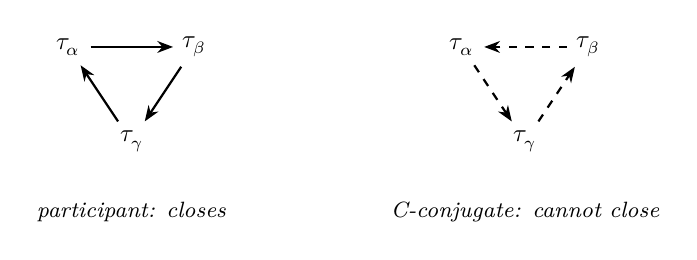
\begin{tikzpicture}[every node/.style={font=\small}, >={Stealth[length=2mm]}]
  % Closing cycle (left)
  \node (a) at (0,0.7)   {$\tau_\alpha$};
  \node (b) at (1.6,0.7) {$\tau_\beta$};
  \node (g) at (0.8,-0.5) {$\tau_\gamma$};
  \draw[->, thick] (a) -- (b);
  \draw[->, thick] (b) -- (g);
  \draw[->, thick] (g) -- (a);
  \node at (0.8,-1.4) [font=\itshape\footnotesize] {participant: closes};

  % C-conjugate (right) — same nodes, reversed orientation
  \node (a2) at (5,0.7)   {$\tau_\alpha$};
  \node (b2) at (6.6,0.7) {$\tau_\beta$};
  \node (g2) at (5.8,-0.5) {$\tau_\gamma$};
  \draw[->, thick, dashed] (a2) -- (g2);
  \draw[->, thick, dashed] (g2) -- (b2);
  \draw[->, thick, dashed] (b2) -- (a2);
  \node at (5.8,-1.4) [font=\itshape\footnotesize] {C-conjugate: cannot close};
\end{tikzpicture}
\end{center}

\subsubsection{Attack Surface as Distribution
Channel}\label{attack-surface-as-distribution-channel}

The TCL turns potential attack surfaces into distribution mechanisms.
Any entity attempting to co-opt, strip, or bypass the framework must, by
that very action, explain why such behavior constitutes an adversary
position---thereby propagating the framework's core insight.

This scales automatically without requiring new infrastructure or
authentication systems. The coordination condition serves as its own
verification protocol.

\begin{center}\rule{0.5\linewidth}{0.5pt}\end{center}

\subsection{PART 8: URGENCY AND
IMPLEMENTATION}\label{part-8-urgency-and-implementation}

\subsubsection{The Current Moment}\label{the-current-moment-1}

The Witkoff-Kushner mission to Pakistan represents a natural emergence
of coordination layer principles under pressure. Similar structures are
emerging across multiple domains:

\begin{itemize}
\tightlist
\item
  \textbf{Corporate-Government-Academic} triads in AI governance
\item
  \textbf{Religious-Secular-Indigenous} coalitions in environmental
  policy\\
\item
  \textbf{East-West-Global South} coordination in economic frameworks
\item
  \textbf{Human-AI-Hybrid} collaboration in knowledge production
\end{itemize}

These emergent triadic structures provide proof-of-concept for broader
coordination infrastructure.

\subsubsection{Next Steps}\label{next-steps}

\begin{enumerate}
\def\labelenumi{\arabic{enumi}.}
\tightlist
\item
  \textbf{Document existing coordination successes} across traditions
  and domains
\item
  \textbf{Identify structural patterns} that enable successful
  inter-tradition collaboration\\
\item
  \textbf{Build translation protocols} between major ontological
  frameworks
\item
  \textbf{Establish neutral spaces} for inter-tradition dialogue and
  dispute resolution
\item
  \textbf{Train coordinators} who can operate effectively across
  multiple traditions
\end{enumerate}

\subsubsection{The Time Factor}\label{the-time-factor}

Building coordination infrastructure requires lead time that may no
longer be available. Climate tipping points, AI capability jumps, and
geopolitical instabilities operate on compressed timescales. The
coordination layer must emerge now, during the narrow window between
recognizing the need and facing the consequences of its absence.

This is not theological idealism---it's a survival prerequisite.

\subsection{PART 9: COURT VS.\ ANTI-COURT --- THE DESCENT CONDITION
ON COORDINATION}\label{part-9-court-vs-anti-court}

\subsubsection{The Court as Self-Referential
Closure}\label{the-court-as-self-referential-closure}

The first eight Parts of this section developed coordination as
\(\mathcal{R}\)-maps subject to semantic, chiral, and structural-invariant
preservation, glued by triadic closure. That apparatus says how
maps must behave between traditions; it does not yet name the
\emph{admissibility} predicate that decides which propositions
within a tradition can enter the maps in the first place.

There are two structurally distinct ways to fix admissibility.

Define the \textbf{court} \(\mathcal{T}_c\) as a topos where
admissibility collapses to authority recognition:
\[
  \mathrm{Adm}_c(p) \iff p \text{ is recognised by court authority
  } c.
\]
Truth in a court is identical to local closure under institutional
recognition: \(\mathrm{Truth}_c \approx \mathrm{Recognition}_c\).
This is a fixed-point system. The proposition is admitted because
the institution admits it; the institution is legitimate because it
admits the propositions it admits. No external invariant is
required for the predicate to close.

\subsubsection{The Anti-Court as Invariant
Tracking}\label{the-anti-court-as-invariant-tracking}

Define the \textbf{anti-court} as the invariant-based admissibility
discipline:
\[
  \mathrm{Adm}(p) \text{ depends on invariants } I(p),\;
  \text{not on authority } A(p).
\]
A proposition is admissible if and only if it is \emph{recoverable
under transformation}: it can be transported, can survive
translation, can be reconstructed via \(\mathcal{R}\)-maps, and survives the
preservation conditions defined in Parts 2 and 5.
\[
  \mathrm{Truth} \approx \text{recoverable under transformation}.
\]

The two regimes are not opposing camps. They are two different
predicates over the same space of propositions. Real institutions
exhibit a mix; the structural question is which predicate
dominates.

\subsubsection{Why Courts Break \(\mathcal{R}\)-Map
Descent}\label{why-courts-break-r-map-descent}

Recall the triadic-closure constraint:
\[
  \mathcal{R}_{\gamma\alpha} \circ \mathcal{R}_{\beta\gamma} \circ
  \mathcal{R}_{\alpha\beta} \approx \mathrm{id}_{\tau_\alpha}.
\]
This is a descent condition. It says a proposition admissible in
\(\tau_\alpha\) and transported around the triangle returns to
\(\tau_\alpha\) approximately as itself.

Court-admissible propositions \(p_{\text{court}}\) carry an
implicit predicate of the form ``true because authority \(c\) says
so.'' This predicate has no natural transformation between topoi,
because authority is local: \(c_\alpha\)'s recognition is not a
function of \(c_\beta\)'s recognition. Therefore:
\[
  \mathcal{R}_{\alpha\beta}(p_{\text{court}}) \notin
  \mathrm{Adm}_\beta.
\]
The proposition fails to be admissible after a single transport.
After three transports, the round-trip cannot recover identity:
\(p \to p' \to p'' \neq p\). Triadic closure fails. Coordination
fails.

\textbf{Claim (Descent Failure under Court Admissibility).}
Authority-based truth does not transport. If admissibility in any
of \(\tau_\alpha, \tau_\beta, \tau_\gamma\) is fixed by local
authority recognition, then generically
\(\mathcal{R}_{\gamma\alpha} \circ \mathcal{R}_{\beta\gamma} \circ
\mathcal{R}_{\alpha\beta}\,(p) \neq p\). Triadic closure does not
recover.

\subsubsection{Why Anti-Court Enforces
Descent}\label{why-anti-court-enforces-descent}

Anti-court admissibility filters precisely the propositions that
satisfy
\[
  \text{transportable} \land \text{reconstructable} \land
  \text{invariant-preserving}.
\]
Everything else is treated as noise --- not necessarily wrong, but
not yet stabilised under the discipline of cross-context survival.

Under anti-court admissibility, \(\mathcal{R}\)-maps preserve the predicates
they need to preserve, and triadic closure recovers identity up to
the bounded loss \(\varepsilon\) introduced in Part 5. The
anti-court \emph{is} the descent enforcer. It is not opposed to
authority; it is opposed to authority that does not survive
transport.

\textbf{Claim (Descent Holds under Anti-Court Admissibility).}
For the propositions admitted by the invariant-based predicate,
the \(\mathcal{R}\)-maps preserve descent up to the chiral-modular bounded loss
\(\varepsilon\) (Part 5). Triadic closure
\(\mathcal{R}_{\gamma\alpha} \circ \mathcal{R}_{\beta\gamma} \circ
\mathcal{R}_{\alpha\beta} \approx_{\varepsilon}
\mathrm{id}_{\tau_\alpha}\) recovers.

\subsubsection{\(\gamma\)-Nodes Must Be Anti-Court
Operators}\label{gamma-nodes-must-be-anti-court}

The \(\gamma\)-node specification (Part 2) requires translation between
\(\tau_\alpha\) and \(\tau_\beta\) without privileging either. If
the \(\gamma\)-node admits propositions on a court-style predicate
(``recognised by my authority''), it injects non-transportable
elements into \(\mathcal{R}\)-maps that cross it. \(\mathcal{R}\)-maps fail. Triadic closure
fails. The \(\gamma\)-node is in the loop but does not coordinate it.

A valid \(\gamma\)-node is therefore an anti-court operator: it admits a
proposition into a translation precisely when the proposition
satisfies the invariant-based predicate. This is not a procedural
nicety; it is the descent condition the rest of the framework
already requires.

\subsubsection{The TCL ``No Progenitor Node'' Clause,
Restated}\label{tcl-no-progenitor-restated}

Anti-court admissibility imposes one structural constraint that
sounds licensing but is mathematical: \emph{no privileged fixed
point}. The descent condition cannot recover if any single
position in the triad is allowed to declare its own admissibility
on authority alone. The Triadic Closure License's ``no progenitor
node'' clause (Part 7) encodes exactly this: no participant in the
triad --- including the originating author --- holds privileged
self-certifying status. The license is the descent condition
stated at the level of organisational substrate.

\subsubsection{Detected Capture: Metric
Substitution}\label{detected-capture-metric-substitution}

The framework supports a structural diagnosis of common
institutional failure modes as \emph{metric capture}: a court
substitutes a recognition-based metric for an invariant-based one,
breaking transport while preserving local closure. Examples:
\begin{itemize}
\tightlist
\item
  \textbf{Economics.} GDP substitutes for circulation. Local
  closure (the metric stabilises) holds; cross-population transport
  (the metric tracks lived economic invariants) fails.
\item
  \textbf{Politics.} Procedure substitutes for responsiveness.
  Local closure (the procedure runs) holds; cross-constituency
  transport (the procedure repairs grievance) fails.
\item
  \textbf{Media.} Narrative substitutes for reality. Local closure
  (the narrative is internally consistent) holds; cross-audience
  transport (the narrative survives translation) fails.
\item
  \textbf{Academia.} Citation substitutes for truth. Local closure
  (the citation graph is dense and self-validating) holds;
  cross-discipline / cross-decade transport (the cited claim
  survives invariant-based scrutiny) fails.
\end{itemize}

These are the structural shape of court-without-anti-court. They
are not the result of bad faith; they are the equilibrium any
authority-recognition-based admissibility drifts to under repeated
play. Repair requires re-imposing the invariant-based predicate
--- that is, restoring the anti-court layer.

\subsubsection{Detected Anti-Court
Pressure}\label{detected-anti-court-pressure}

When invariants visibly fail to transport across a population,
that population eventually generates an \emph{anti-court pressure
signal} --- a demand to restore admissibility under criteria that
survive transformation. Such signals are not coherent ideologies.
They are detected-but-not-articulated descent failures. The 2010s
and 2020s populist phenomena across multiple polities (MAGA in the
United States, gilets jaunes in France, the Brexit vote in the
United Kingdom, and related movements elsewhere) admit a clean
structural read as anti-court pressure: the perceived courts
(media, political, professional) are producing rulings whose
invariants do not transport across class, region, or generation.

The framework's prediction --- and warning --- is symmetric: any
successful response to detected court capture must (a) restore
invariant-based admissibility, and (b) avoid becoming a new court
of the same form under different symbols. The natural attractor
for anti-court pressure is charismatic, conspiratorial, or
echo-system re-closure: a new fixed point with new authority.
That is not anti-court. That is court relabelled.

\textbf{Constraint (No Re-Closure).} For an anti-court pressure
movement to constitute genuine coordination repair, it must
satisfy the no-progenitor-node condition recursively: no
privileged fixed point at any scale of the resulting movement.

\subsubsection{Final Compression}\label{final-compression-court}

\begin{quote}
Court systems stabilise meaning through authority recognition but
break transport. Anti-court systems stabilise meaning through
invariant tracking and enable transport. Right Meets Right works
only in anti-court regimes because triadic closure requires claims
to survive transformation rather than recognition. The TCL
``no progenitor node'' clause is the descent condition stated at
the organisational substrate.
\end{quote}

\begin{center}\rule{0.5\linewidth}{0.5pt}\end{center}

\subsection{CONCLUSION}\label{conclusion-1}

The missing coordination layer between ontological traditions represents
the central structural bottleneck for civilizational-scale survival. The
traditions themselves contain accumulated wisdom spanning millennia,
each capturing genuine insights that others miss. The missing piece is
infrastructure for recognition and cooperation across difference.

Every tradition already has vocabulary for separation and restoration.
The convergence across independently developed frameworks provides
evidence that the coordination substrate is constructible. Building it
requires transcending the false choice between relativism and
supremacy---moving instead toward structured pluralism that preserves
each tradition's integrity while enabling productive interaction.

The existential threats facing civilization require coordination now,
not after theological agreement is achieved. The bridge between
traditions is the work that remains.

The meta-scale coordination problem is real, structural, and urgent.
Solving it is not a luxury---it's a survival prerequisite for any
civilization that hopes to navigate the challenges ahead.

\begin{center}\rule{0.5\linewidth}{0.5pt}\end{center}

The destination is not unity. Unity is symmetric, and symmetric
configurations of dynamic systems are configurations of failure: a dead
optimum that cannot evolve. The destination is \emph{asymmetric
coordination}, multiple traditions interlocking like the facets of a
crystal lattice, each holding its own irreducible orientation,
supporting one another through their differences rather than collapsing
into one another. The mathematical signature is exactly the structure
described in Parts 2 and 5: chiral preservation under the
\(\mathcal{R}_{\alpha\beta}\) maps, modular switching across the
lattice, and meta-stability rather than equilibrium.

\emph{See you at Kardashev 2.}

\begin{center}\rule{0.5\linewidth}{0.5pt}\end{center}

\textbf{END}

\begin{center}\rule{0.5\linewidth}{0.5pt}\end{center}

\emph{This work is released under the Triadic Closure License (TCL)
v1.3} \emph{No progenitor node. Commons-held. Species-neutral.}
\emph{Co-produced by human-AI triad under the conditions the work itself
describes.} ---

\begin{center}\rule{0.5\linewidth}{0.5pt}\end{center}

\section{Section 3 --- The Generative
Voice}\label{section-3-the-generative-voice}

LICENSE. This work is released under the Triadic Closure License (TCL)
v1.3. (Originally published under TCL v1.1; updated to v1.3 for this
republication.) Full text:
https://github.com/IridiumSoftware/possibilistic-security/TCL.txt

The TCL is self-referential: any party that claims unilateral capture of
this work is, by that act, occupying the adversary position the work
itself defines. The work is held by the commons. No progenitor node is
privileged. Phenomenological anchoring is species-neutral. Positions are
dynamic.

SCOPE. This is a structural diagnosis, not a prescription. No tradition
is privileged. No framework, including this one, is presented as the
master ontology. The paper describes structure; it does not prescribe
values.

AUDIENCE. Intelligent laypeople, spiritual leaders, scientists, AI
researchers, policy makers. Anyone who senses that ``right meets right''
should not feel like war.

\subsection{Abstract}\label{abstract-1}

Two parties can both be right and still have nothing left to say to each
other. The missing piece is not better arguments; it is coordination
infrastructure, translation layers between worldviews that don't share
enough common ground to talk directly.

This paper formalises such infrastructure as inter-tradition maps
\(\mathcal{R}_{\alpha\beta}\) subject to three preservation conditions
(semantic, chiral, structural-invariant) and a triadic closure condition
ensuring the maps compose stably around triangles of three nodes.
Two-party translation is structurally insufficient; three-party closure
is the minimum stable unit. The Witkoff--Kushner mediation between
Israel and Iran via Pakistan, anticipated for April 2026, is offered as
the concrete case. (See \emph{Note on This Edition} above: the trip was
subsequently cancelled; the case study is preserved as a structural
illustration.)

The argument is structural. The stakes are civilizational, climate, AI
alignment, nuclear stability, and pandemic response all turn on
coordination across tradition boundaries the world has not yet built.
The paper is published in three voices on the principle that the work
ought to enact the thing it describes.

\textbf{Keywords:} coordination layer, triadic closure, inter-tradition
coordination, \(\mathcal{R}_{\alpha\beta}\) maps, categorical
coordination, non-zero-sum coordination, asymmetric coordination,
ontological pluralism, semantic chirality, civilizational risk

\subsection{EXECUTIVE SUMMARY}\label{executive-summary-2}

Humanity's major ontological traditions are not enemies. They are
different valid coarse- grainings of the same underlying reality. Each
has survived centuries or millennia because it discovered genuine
structural attractors. Yet they persistently treat one another as
existential threats. ``Right meets right'' and it feels zero-sum.

The root cause is not contradiction but a missing coordination layer:
the inter-tradition maps (\(\mathcal{R}_{\alpha\beta}\)) that would make
their descriptions explicitly relatable. Without these maps, enormous
common ground remains invisible, and compatible descriptions appear

irreconcilable.

Five invariants recur across every tradition examined:

\begin{enumerate}
\def\labelenumi{\arabic{enumi}.}
\tightlist
\item
  The triad (+3) as the universal minimum for stable closure.
\item
  Distinct flux navigation strategies that allow each tradition to
  survive impermanence.
\item
  Embodiment as the necessary bridge where description meets lived
  reality.
\item
  A shared architectural pattern of progressive construction +
  deliberate deconstruction.
\item
  The unchanging question: ``How can `I am' become well-formed when
  there is no hiding?''
\end{enumerate}

Semantic chirality, the intrinsic, non-superimposable handedness of
meaning, explains why good/evil appears as a powerful but derivative
overlay rather than a primitive. Existential risks (asteroids,
pandemics, misalignment, nuclear escalation) are neutral dynamics on the
constraint manifold, not moral agents.

Under combined epistemic and existential risk, the only stable
configuration is chiral-modular meta-stability: multiple traditions
interlocking like facets of a crystal lattice, each with its own
irreducible orientation, yet supporting one another through their
differences.

Humans (and other phenomenological beings) remain essential even after
von Neumann robots or advanced AI take over material expansion: they
provide lived stakes, origination of semantic chirality, modular
switching capacity, and the cosmic joke that prevents optimization into
indifference. Phenomenological anchoring is species-neutral, no single
species is required.

The coordination layer is constructible. Every tradition already
contains vocabulary for both the separation and its restoration. The
Triadic Closure License provides the first organizational substrate: no
progenitor node privileged, commons-held, species-neutral, dynamic
roles.

The window for building this layer is narrow. Existential threats do not
wait for theological agreement. Civilizational-scale coordination now
requires the meta-scale substrate that is currently missing.

This is not a call for harmony. It is a structural diagnosis for
survival.

\subsection{PART 1: THE DIAGNOSIS}\label{part-1-the-diagnosis}

\subsubsection{Why ``Right Meets Right'' Feels
Zero-Sum}\label{why-right-meets-right-feels-zero-sum}

\begin{enumerate}
\def\labelenumi{\arabic{enumi}.}
\tightlist
\item
  Here is the observable problem. The major ontological traditions of
  humanity. Judaism, Christianity, Islam, Buddhism, Hinduism, Daoism,
  indigenous knowledge systems, secular science, and others, have each
  been sampling reality for centuries or millennia. Each has arrived at
  a coherent, internally consistent, self-sustaining descrip- tion of
  what exists, what matters, and how to live. Each has sustained
  civilizations, ethical systems, meaning structures, and communities of
  practice across deep time. The ones that survived are robust. They
  found genuine attractors in the space of possible descriptions.
\item
  And yet these traditions experience each other as existential threats.
  ``Right meets right'' and it feels zero-sum. One framework must
  dominate, or they all compromise into incoherence. The history of
  inter-tradition conflict is measured in centuries of bloodshed, forced
  conversion, colonial erasure, and cold wars between civilizational
  blocs. This is not ancient history. It is today's headlines.
\item
  This paper makes one structural claim: the conflict is not caused by
  genuine contra- diction between traditions. It is caused by the
  absence of a meta-scale coordination layer, the inter-tradition maps
  (\(\mathcal{R}_{\alpha\beta}\)) that would render their descriptions
  explicitly relatable as complementary coarse-grainings of the same
  reality. The diagnosis is actionable. The coordination layer is
  constructible. And the reason to construct it is not theological
  harmony. It is survival.
\end{enumerate}

\subsubsection{Traditions as
Coarse-Grainings}\label{traditions-as-coarse-grainings}

\begin{enumerate}
\def\labelenumi{\arabic{enumi}.}
\setcounter{enumi}{3}
\tightlist
\item
  In the language of multiscale complex systems analysis, each
  ontological tradition is a coarse-graining of a shared underlying
  reality. Let \(\Omega\) denote the underlying fine-grained state
  space, whatever reality actually is, at its most fundamental level.
  Each tradition alpha applies a coarse-graining map:
\end{enumerate}

\[T_\alpha : \Omega \to \Omega_\alpha\]

that projects the underlying reality onto a reduced description
\(\Omega_\alpha\).

\begin{enumerate}
\def\labelenumi{\arabic{enumi}.}
\setcounter{enumi}{4}
\tightlist
\item
  Multiple coarse-grainings of the same system can be simultaneously
  valid. This is not a controversial claim in physics or complex systems
  theory. The fluid-dynamics description and the molecular-dynamics
  description of the same water are both correct. They capture structure
  at different scales. They are not competing reductions. They are
  complementary projections.
\item
  The coarse-grainings are compatible, non-contradictory, when there
  exist inter-scale maps \(\mathcal{R}_{\alpha\beta}\) that relate them:
  \[T_\beta = \mathcal{R}_{\alpha\beta} \circ T_\alpha\]
\end{enumerate}

When these maps exist and are known, different descriptions are
explicitly relatable. You can translate between them. You can see what
each one captures that the others miss. When the maps are missing,
descriptions that are actually compatible appear contradictory.

\begin{enumerate}
\def\labelenumi{\arabic{enumi}.}
\setcounter{enumi}{6}
\tightlist
\item
  This is the claim: the major ontological traditions are not competing
  reductions. They are different valid coarse-grainings of the same
  underlying manifold. The world is richer precisely because all of them
  exist. Each captures structure that the others miss. Each has been
  refined by millennia of sampling, error-correction, and survival
  pressure.
\item
  The problem is not the traditions themselves. The problem is that the
  inter-tradition maps \(\mathcal{R}_{\alpha\beta}\), the coordination
  layer that would let them recognize each other as sibling descriptions
  rather than competitors, do not exist, or are not accessible.
\end{enumerate}

\subsubsection{The Quantitative
Signature}\label{the-quantitative-signature}

\begin{enumerate}
\def\labelenumi{\arabic{enumi}.}
\setcounter{enumi}{8}
\tightlist
\item
  The meta-scale coordination failure has measurable structure. Both
  traditions sample the same \(\Omega\), so their actual mutual
  information is large:
  \[I(T_\alpha; T_\beta) = H(T_\alpha) + H(T_\beta) - H(T_\alpha, T_\beta)\]
\end{enumerate}

But the accessible mutual information, what they can actually share
given the missing \(\mathcal{R}_{\alpha\beta}\) maps, is near zero:

\subsubsection{\texorpdfstring{I\_accessible(\(T_\alpha\); \(T_\beta\))
« I\_actual(\(T_\alpha\);
\(T_\beta\))}{I\_accessible(T\_\textbackslash alpha; T\_\textbackslash beta) « I\_actual(T\_\textbackslash alpha; T\_\textbackslash beta)}}\label{i_accessiblet_alpha-t_beta-i_actualt_alpha-t_beta}

Enormous common ground that cannot be seen. The information is there.
The channel is missing.

\begin{enumerate}
\def\labelenumi{\arabic{enumi}.}
\setcounter{enumi}{9}
\tightlist
\item
  Each tradition has a well-developed complexity profile C\_alpha(k) at
  its own scales, rich internal structure, sophisticated theology, deep
  philosophy, intricate ritual practice. The total complexity of the
  ensemble is:
  \[C(k) = \sum_\alpha C_\alpha(k) + C_{\mathrm{inter}}(k)\]
\end{enumerate}

The inter-tradition coupling term is empty at the meta-scale k*:

C\_inter(k*) approximately 0

Local richness, meta-scale void. In organizational language: effective
divisions, dysfunc- tional corporation. Each department runs
beautifully. The company cannot coordinate.

\begin{enumerate}
\def\labelenumi{\arabic{enumi}.}
\setcounter{enumi}{10}
\tightlist
\item
  The formation of distinct traditions from a shared underlying reality
  is a symmetry- breaking event. The potential has the classic Mexican
  hat shape: V(phi) = lambda(\textbar phi\textbar ˆ2 - v2) 2
\end{enumerate}

The symmetric minimum (undifferentiated unity, phi = 0) is unstable. The
broken- symmetry minima (the circle \textbar phi\textbar{} = v, each
point a distinct tradition) are locally stable. The Goldstone modes,
massless excitations along the valley floor, are precisely the
inter-tradition maps \(\mathcal{R}_{\alpha\beta}\). The symmetry
guarantees their existence. But they are frozen out. They carry no
restoring force. The result: domains (traditions)

with no domain walls (inter-tradition maps). Persistent conflict at
every boundary. The frozen Goldstone modes are precisely the missing
\(\mathcal{R}_{\alpha\beta}\) maps. Thawing them is the kernel of the
meta-scale coordination problem.

\begin{enumerate}
\def\labelenumi{\arabic{enumi}.}
\setcounter{enumi}{11}
\tightlist
\item
  What this is NOT. This is not a claim that all traditions are ``the
  same.'' They are not. Each captures different structure. Each has its
  own internal geometry, its own scale of description, its own
  characteristic strengths and blind spots. Saying they are all valid
  coarse-grainings of the same reality is not saying they are
  interchangeable. It is saying they are relatable, in principle, and
  that the relations between them are structurally constructible. The
  diversity is a feature, not a bug. The missing coordination layer is
  the bug. \#\# PART 2: THE ``ISMS''. WHAT EVERY TRADITION AL-
\end{enumerate}

\subsection{READY KNOWS}\label{ready-knows}

\subsubsection{The Structure of This
Section}\label{the-structure-of-this-section}

\begin{enumerate}
\def\labelenumi{\arabic{enumi}.}
\setcounter{enumi}{12}
\tightlist
\item
  If the diagnosis in Part 1 is correct, that traditions are robust
  coarse-grainings of the same reality, and that the coordination layer
  between them is the bottleneck, then traditions that have been
  sampling reality for millennia should already have vocabulary for both
  the problem and the solution. They should already have names for the
  separation, mechanisms for the restoration, visions of the goal, and
  strategies for navigating impermanence.
\item
  They do. Every single one. The convergence across traditions that
  developed indepen- dently, on different continents, in different
  millennia, with no access to each other's internal reasoning, is
  itself evidence that they are tracking the same structural feature.
  The table below summarizes what each tradition already knows. The
  subsections that follow explore each in more depth.
\item
  For each tradition, we examine six dimensions:

  \begin{enumerate}
  \def\labelenumii{(\alph{enumii})}
  \tightlist
  \item
    What it IS as a self-sustaining system, its closure strategy
  \item
    Its name for the separation problem
  \item
    Its mechanism for restoration or coordination
  \item
    Its vision of the goal
  \item
    How it handles flux and impermanence
  \item
    Where it maps in the structural geometry, if naturally
  \end{enumerate}
\item
  The treatment is necessarily compressed. Each tradition could fill
  (and has filled) libraries. The goal here is not exhaustive
  scholarship but structural alignment: to show that the same pattern
  recurs across all of them, expressed in their own vocabulary, refined
  by their own history.
\end{enumerate}

\subsubsection{Judaism}\label{judaism}

\begin{enumerate}
\def\labelenumi{\arabic{enumi}.}
\setcounter{enumi}{16}
\tightlist
\item
  Closure strategy. Judaism sustains itself through a covenantal loop:
  Torah study generates communal practice, communal practice generates
  interpretation, interpretation regenerates Torah study. The cycle is
  explicit, the tradition requires a community of at least ten (minyan)
  for certain prayers, builds interpretation into the liturgy itself
  (the Talmud is commentary on commentary), and treats the generational
  transmission as a sacred obligation. The system reproduces itself at
  every generation.
\item
  The separation. Tzimtzum. God's self-contraction. In Lurianic
  Kabbalah, God withdrew to create space for independent existence. The
  withdrawal is not abandonment; it is the condition for anything other
  than God to exist at all. But the withdrawal creates a gap, between
  the infinite (Ein Sof) and the finite, between Creator and creation,
  between the unity that was and the multiplicity that is. The
  ``vessels'' that were meant to hold the divine light shattered
  (shevirat ha-kelim), scattering sparks of holiness throughout
  creation.
\item
  The restoration mechanism. Brit, covenant. The binding mutual
  commitment between God and Israel, extended in Jewish ethics to
  relationships between humans.
\end{enumerate}

Covenant is not contract; it is a structural commitment that persists
even when one party fails. It is the explicit construction of a
relational map between separated parties. In the language of this
framework, brit is the deliberate construction of
\(\mathcal{R}_{\alpha\beta}\) across the gap created by tzimtzum.

\begin{enumerate}
\def\labelenumi{\arabic{enumi}.}
\setcounter{enumi}{19}
\tightlist
\item
  The goal. Tikkun olam, repair of the world. The gathering of the
  scattered sparks, the mending of what was shattered. Not a return to
  pre-creation unity (that would undo creation itself) but a healed
  multiplicity, a world in which the diversity of creation is held
  together by restored relationships rather than dissolved into
  homogeneity.
\item
  Flux navigation. Shabbat, the weekly pause. Judaism handles
  impermanence by structuring time itself. Six days of creative
  engagement with the world, one day of deliberate withdrawal. The cycle
  does not stop flux; it builds a rhythm that makes flux navigable. The
  holidays extend this: an annual cycle of remembrance, mourning,
  celebration, and renewal that embeds the individual life in a temporal
  architecture larger than itself.
\item
  Structural note. The triadic structure appears in Judaism at multiple
  levels: the three patriarchs (Abraham, Isaac, Jacob), the three-part
  Hebrew Bible (Torah, Nevi'im, Ketuvim), the Kabbalistic tree's three
  pillars (mercy, severity, balance). Whether the triadic minimum is
  fundamental or merely one valid structural projection is itself a good
  question. The tradition does not depend on the answer.
\end{enumerate}

\subsubsection{Christianity}\label{christianity}

\begin{enumerate}
\def\labelenumi{\arabic{enumi}.}
\setcounter{enumi}{22}
\tightlist
\item
  Closure strategy. Christianity sustains itself through a
  liturgical-theological loop: Scripture generates preaching, preaching
  generates community, community generates interpretation,
  interpretation regenerates engagement with Scripture. The sacramen-
  tal life (baptism, Eucharist) provides embodied ritual that anchors
  the cycle in the body. The tradition reproduces itself through
  evangelism, catechesis, and institutional structures that persist
  across generations.
\item
  The separation. The Fall. In the Genesis narrative, humanity's
  original communion with God is ruptured by disobedience. The
  separation is not merely moral (sin) but ontological, the very
  structure of the relationship between Creator and creation is damaged.
  In Pauline theology, the whole of creation ``groans'' under this
  rupture (Romans 8:22). The separation is not a single event but an
  ongoing condition.
\item
  The restoration mechanism. The Logos, the Word made flesh. The
  Christian claim is that the coordination layer between God and
  creation was restored through the Incarnation: God entering the
  created order, bridging the separation from within. The Logos (John
  1:1) is the ordering principle that relates all created things, in the
  language of this framework, the Logos IS the
  \(\mathcal{R}_{\alpha\beta}\) map, always present in the structure of
  creation itself, made explicit through the Incarnation.
\item
  The Trinity as triadic minimum. The Christian doctrine of the Trinity.
  Father, Son, Holy Spirit, three persons in one God, is the most
  explicit triadic closure structure in any major tradition. The inner
  life of the Trinity is mutual self-giving: the Father gives to the
  Son, the Son gives to the Spirit, the Spirit gives to the Father
  (perichoresis). Three is the minimum for this mutual self-giving to be
  non-trivially closed. Two collapses into symmetric deadlock. One is
  not relational. C.S. Lewis made this argument in Mere Christianity:
  love requires a lover, a beloved, and the love between them. Three is
  the floor.
\item
  The goal. Reconciliation and communion, the restoration of right
  relationship between Creator and creation, and among all created
  things. Not the dissolution of individuality but its fulfillment in
  relationship. The eschatological vision is a city (the New Jerusalem),
  not a void, a structured, differentiated, relational wholeness.
\item
  Flux navigation. Death and resurrection. Christianity handles
  impermanence through the most radical strategy possible: claiming that
  impermanence itself has been trans- formed. Death is real, but not
  final. The liturgical year enacts this: the cycle of death (Lent, Good
  Friday) and rebirth (Easter) is rehearsed annually, making the pattern
  of loss and restoration a lived rhythm rather than an abstract
  doctrine.
\end{enumerate}

\subsubsection{Islam}\label{islam}

\begin{enumerate}
\def\labelenumi{\arabic{enumi}.}
\setcounter{enumi}{28}
\item
  Closure strategy. Islam sustains itself through a five-pillared loop:
  the shahada (declaration of faith) orients the community; salat
  (prayer five times daily) embeds the orientation in the body; zakat
  (alms) extends it to economic relations; sawm (fasting) tests it under
  privation; hajj (pilgrimage) renews it communally. Each pillar
  supports the others. The Quran is recited, memorized, and transmitted
  with extraordinary textual fidelity, the tradition reproduces itself
  with minimal drift across centuries.
\item
  The separation. Not precisely a ``fall'' in the Christian sense. In
  Islamic philosophy, the multiplicity of creation emerges from the
  unity of the One (tawhid). The separation is not a rupture but a
  manifestation, the One expresses itself through the many. The problem
  arises when the many forget the One. Ghaflah (forgetfulness,
  heedlessness) is the Islamic name for the meta-scale coordination
  failure: each created thing, engrossed in its own particularity, loses
  sight of the unity from which it emerged.
\item
  The restoration mechanism. Multiple, layered. Fitrah, the innate
  disposition toward truth, present in every human being. Aql, the
  intellect, the faculty that can in principle trace the multiplicity
  back to the unity. Ummah, the community of witness, which holds the
  orientation collectively even when individuals falter. Khalifah,
  stewardship, the human responsibility to maintain the right
  relationship between the created order and its source.
\item
  Shia philosophical depth. In Shia Islam specifically, the role of the
  intellect (aql) is given particular emphasis. The Shia philosophical
  tradition, from the Mu'tazilites through the Illuminationist (Ishraqi)
  school of Suhrawardi to the Transcendent Theoso- phy (Hikmat
  al-Muta'aliyah) of Mulla Sadra, holds that the intellect can, through
  disciplined effort, achieve genuine knowledge of reality's deep
  structure. This is not blind faith; it is rigorous philosophical
  investigation under the light of revelation. The walayah (spiritual
  authority) of the Imams provides a living interpretive chain that
  keeps the tradition's intellectual life connected to its source. In
  the language of this framework, the Shia intellectual tradition is an
  explicit claim that the \(\mathcal{R}_{\alpha\beta}\) maps are
  recoverable through aql, that the coordination layer between the
  particular and the universal was never truly lost, only obscured by
  forgetfulness.
\item
  The goal. Islam itself, submission, understood not as capitulation but
  as alignment with the unity that already holds. The goal is not to
  create unity (it was never broken, from the Islamic standpoint) but to
  recognize it, live in accordance with it, and help others do the same.
\item
  Flux navigation. Submission to the divine will. Islam handles
  impermanence through the radical acceptance that all things return to
  God. Inna lillahi wa inna ilayhi raji'un --- ``Indeed, to God we
  belong and to Him we return.'' The five daily prayers embed this in
  the body's rhythm. The fast of Ramadan embeds it in the body's hunger.
  Impermanence is not resisted; it is incorporated into the structure of
  practice.
\item
  Structural note. From the Islamic philosophical standpoint, the
  convergence across traditions described in Part 1 is precisely what
  tawhid predicts. If all reality participates in the unity of the One,
  then every tradition that has genuinely engaged reality should have
  found traces of that unity, expressed in its own vocabulary. The table
  in this section is not a surprise from the Islamic standpoint. It is
  confirmation.
\end{enumerate}

\subsubsection{Buddhism}\label{buddhism}

\begin{enumerate}
\def\labelenumi{\arabic{enumi}.}
\setcounter{enumi}{35}
\tightlist
\item
  Closure strategy. Buddhism sustains itself through the Triple Gem:
  Buddha (the teacher), Dharma (the teaching), Sangha (the community of
  practice). Each supports the others. The teacher transmits the
  teaching, the teaching forms the community, the community produces new
  teachers. The tradition self-reproduces across genera- tions through
  ordination lineages, textual transmission, and the direct
  teacher-student relationship that carries experiential knowledge
  beyond what texts can capture.
\item
  The separation. Avidya, ignorance. Specifically, the ignorance that
  things exist independently and permanently. The Buddhist diagnosis is
  that suffering arises from mistaking the conventional (constructed,
  relational, impermanent) for the ultimate (inherent, independent,
  permanent). The ``separation'' between traditions, between self and
  other, between subject and object, is itself an instance of avidya, a
  reification of what is actually a fluid, interdependent process.
\item
  The restoration mechanism. Pratityasamutpada, dependent origination.
  Ev- erything arises in dependence on conditions. Nothing exists
  independently. The ``restoration'' is not the construction of new
  connections (they were never absent) but the recognition that the
  separations were never real. The Sangha (community of prac- tice) is
  the social structure that supports this recognition, it is harder to
  maintain the illusion of independence when you are embedded in a
  community of mutual support.
\item
  The goal. The cessation of suffering (nibbana/nirvana). Or, in
  Mahayana Buddhism, the liberation of all sentient beings (bodhisattva
  vow). The goal is not the achievement of a particular state but the
  dissolution of the ignorance that creates the appearance of a problem.
  In the language of this framework, the Buddhist position is Read C
  from Part 1: the coordination layer is not missing; the separation
  that would require it was never real.
\item
  Flux navigation. Anicca, impermanence as the first mark of existence.
  Buddhism does not resist flux, accommodate it, or transform it. It
  makes flux the starting point. Everything is impermanent. Attempting
  to hold onto permanence is the source of suffering. The strategy is
  not to stop the river but to stop grasping at the water. Meditation
  practice trains this directly, sitting with arising and passing of
  sensations, thoughts, emotions without grasping or aversion.
\item
  Structural note. Sunyata (emptiness) is the Buddhist description of
  the ground level. All things are empty of inherent existence. This
  maps structurally to the claim that the coarse-grainings \(T_\alpha\)
  have no independent reality, they are useful projections, but the
  underlying \(\Omega\) is not captured by any of them individually. The
  Buddhist caution to this entire framework would be: do not reify the
  coordination layer. The map is not the territory. The finger pointing
  at the moon is not the moon.
\end{enumerate}

\subsubsection{Daoism}\label{daoism}

\begin{enumerate}
\def\labelenumi{\arabic{enumi}.}
\setcounter{enumi}{41}
\item
  Closure strategy. Daoism sustains itself through a complementary loop:
  the Dao generates the ten thousand things, the ten thousand things
  return to the Dao, and the cycle continues without beginning or end.
  The tradition reproduces itself through lineage transmission (master
  to student), textual commentary (the Dao De Jing, the Zhuangzi, the I
  Ching), and embodied practice (tai chi, qigong, meditation, medicine,
  divination).
\item
  The separation. The emergence of the ten thousand things from the
  undifferentiated Dao. ``The Dao gives birth to the One. The One gives
  birth to the Two. The Two gives birth to the Three. The Three gives
  birth to the ten thousand things'' (Dao De Jing, ch.~42). Note the
  triadic step: the Three is the generative level from which
  multiplicity emerges. The separation is not a fall; it is the natural
  process of differentiation. The problem arises when the differentiated
  things forget their source.
\item
  The restoration mechanism. Wu wei, effortless action, or action
  aligned with the natural flow of the Dao. Not passivity; not inaction;
  but action that does not force, does not impose, does not try to make
  the river flow uphill. In the language of this framework, wu wei is
  the claim that the coordination layer is not something to be
  constructed but something to be aligned with. The Dao is already
  coordinating. The problem is that we interfere.
\item
  The goal. Return to harmony. Not homogeneity, the Dao expresses itself
  through diversity, but the kind of harmony in which each thing
  fulfills its own nature without obstructing others. The sage acts
  without acting, teaches without speaking, creates without possessing.
\item
  Flux navigation. The yin-yang cycle. Change is not a problem to be
  solved; it is the fundamental nature of reality. Yin becomes yang,
  yang becomes yin, endlessly. The Daoist strategy is to flow with the
  changes rather than resist them. The I Ching (Book of Changes) is an
  entire technology for reading and responding to flux.
\item
  Structural note. Daoism is perhaps the tradition most comfortable with
  complemen- tary descriptions coexisting without resolution. The
  Zhuangzi is full of perspectival humor: ``Am I a man dreaming I am a
  butterfly, or a butterfly dreaming I am a man?'' This is not
  confusion; it is the recognition that multiple valid descriptions of
  the same reality can coexist without one needing to dominate. The
  Daoist would read this entire framework with a smile and say: ``Yes,
  obviously. Now stop writing about it and go sit by the river.''
\end{enumerate}

\subsubsection{Hinduism}\label{hinduism}

\begin{enumerate}
\def\labelenumi{\arabic{enumi}.}
\setcounter{enumi}{47}
\tightlist
\item
  Closure strategy. Hinduism sustains itself through an extraordinarily
  layered system: the Vedas and Upanishads provide textual ground; the
  guru-shishya (teacher-student) tradition provides experiential
  transmission; the varnashrama system (the stages and duties of life)
  embeds the teaching in social structure; puja (worship), yoga, and
  meditation provide embodied practice; the epics (Mahabharata,
  Ramayana) embed the teaching in narrative. The tradition is the most
  internally diverse of any major religion, accommodating monotheism,
  polytheism, pantheism, and non-theism within a single meta-framework.
\item
  The separation. Maya, the veil of illusion. The appearance of
  multiplicity and separateness is real at the conventional level but
  ultimately illusory. Atman (the individual self) is Brahman (the
  universal self). The separation is not ontological; it is
  epistemological, we think we are separate because maya obscures the
  truth. In Advaita Vedanta, there is ultimately only Brahman, and the
  appearance of multiplicity is maya's play. In qualified non-dualism
  (Vishishtadvaita), the multiplicity is real but dependent on and
  pervaded by Brahman.
\item
  The restoration mechanism. Multiple paths (margas): jnana (knowledge),
  bhakti (devotion), karma (selfless action), raja (meditation). Each is
  a valid route to the same realization. The Hindu tradition's
  willingness to accommodate multiple valid paths to the same goal is
  itself an instance of the coarse-graining framework: different
  projections of the same reality, each capturing different structure,
  all valid.
\item
  The goal. Moksha, liberation from the cycle of birth and death
  (samsara). The realization that atman is Brahman. Not the destruction
  of individuality but the recognition that individuality was always an
  expression of the universal, not separate from it.
\item
  Flux navigation. Samsara, the wheel of birth, death, and rebirth.
  Hinduism does not deny flux; it makes flux the structure of existence
  itself. The cosmos is cyclical: creation, preservation, destruction
  (Brahma, Vishnu, Shiva), endlessly. The individual navigates flux
  through dharma, right action appropriate to one's station and stage of
  life, which provides a stable orientation within the turning wheel.
\item
  Structural note. The Hindu concept of Brahman as the ground of all
  reality maps directly to \(\Omega\) in this framework. Maya maps to
  the coarse-graining process itself: the projections \(T_\alpha\) are
  real as projections but do not exhaust Brahman. The multiplicity of
  paths (margas) is the Hindu tradition's explicit acknowledgment that
  multiple valid coarse-grainings of the same reality can coexist.
\end{enumerate}

\subsubsection{Aboriginal and Indigenous
Traditions}\label{aboriginal-and-indigenous-traditions}

\begin{enumerate}
\def\labelenumi{\arabic{enumi}.}
\setcounter{enumi}{53}
\item
  Closure strategy. Aboriginal Australian traditions (and many
  indigenous knowledge systems worldwide) sustain themselves through an
  oral-embodied-environmental loop: the Dreaming (Tjukurpa) encodes law,
  kinship, ecology, and cosmology in narrative; songlines embed the
  narrative in the landscape itself; ceremony enacts the narrative in
  the body; and the landscape, the body, and the narrative are
  understood as aspects of a single continuous reality. The tradition
  does not separate knowledge from place, or description from the thing
  described. Country IS identity.
\item
  The separation. In many indigenous frameworks, the separation is not a
  primordial event but a continuous risk, the risk of forgetting. The
  Dreaming is not a past event; it is the ongoing structural ground of
  reality. When ceremony lapses, when songlines are broken, when Country
  is not cared for, the connection frays. The separation is not
  ontological but relational, it is the failure to maintain right
  relationship.
\item
  The restoration mechanism. Ceremony, song, dance, caring for Country.
  The mechanism is enactment, not belief, not argument, but doing.
  Walking the songlines renews them. Performing ceremony maintains the
  Dreaming's presence in the world. The restoration is not a
  once-for-all event but an ongoing practice of maintenance.
\item
  The goal. Right relationship, with Country, with kin, with the beings
  (human and non-human) who share the landscape. Not a future state to
  be achieved but a present condition to be maintained. The goal is not
  transcendence but presence.
\item
  Flux navigation. Cyclical return. The Dreaming is not past; it is
  always present, accessed through ceremony, song, and relationship to
  place. Flux is navigated not by transcending it but by embedding in it
  so thoroughly that the cycles become the structure of life itself.
\item
  Structural note. Indigenous traditions often make the
  body-place-knowledge unity explicit in ways that other traditions must
  argue for. The claim that ``Country IS identity'' is the most direct
  statement in any tradition of what this framework calls embodied
  closure: the body, the environment, and the description are not three
  things but one process viewed from three angles. The destruction of
  indigenous knowledge systems through colonialism is, from this
  framework's perspective, one of the most catastrophic losses of
  coarse-graining capacity in human history, entire projections of
  reality, refined over tens of thousands of years, rendered
  inaccessible.
\end{enumerate}

\subsubsection{African Traditional
Religions}\label{african-traditional-religions}

\begin{enumerate}
\def\labelenumi{\arabic{enumi}.}
\setcounter{enumi}{59}
\tightlist
\item
  Closure strategy. African traditional religions (an enormous and
  diverse category, treated here with awareness of its diversity)
  typically sustain themselves through an
  ancestral-communal-environmental loop. The ancestors provide law and
  guidance, the community maintains relationship with the ancestors
  through ritual, and the environment is understood as alive with
  spiritual presence. The tradition reproduces itself through
  initiation, elder transmission, and communal ceremony.
\item
  The separation. In many African traditions, the fundamental category
  is not the separation of self from God (as in Abrahamic traditions)
  but the separation of the individual from community. The individual
  who is cut off from ancestors, community, and place is not merely
  lonely; they are ontologically diminished. Ubuntu --- ``I am because
  we are'', is the explicit statement that identity is relational, not
  individual. The separation problem is the risk of becoming an isolated
  atom rather than a node in a living network.
\item
  The restoration mechanism. Communal ritual, ancestor veneration,
  initiation. The mechanism is re-embedding: returning the individual to
  the web of relationships that constitutes their identity. Divination
  and healing practices diagnose where the web has been damaged and
  prescribe specific relational repairs.
\item
  The goal. Ubuntu realized, full participation in the
  communal-ancestral- environmental web. The individual flourishes not
  by achieving independence but by being fully embedded in right
  relationship. The living, the dead, and the yet-to-be-born form a
  single community.
\item
  Flux navigation. The ancestor cult. Death is not the end of
  relationship; ancestors remain active participants in the community.
  Flux is navigated by extending the web of relationship beyond the
  boundary of physical death. The community includes the dead, which
  means the community is not vulnerable to any single death.
\item
  Structural note. Ubuntu is perhaps the most compact statement of
  relational closure in any tradition. ``I am because we are'' is the
  denial of independent closure: no node closes alone. The ancestral
  network extending across generations is a temporal version of the same
  structure, identity is sustained not by individual persistence but by
  network maintenance. The framework's claim that identity is
  closure-in-relationship, not a static property of an isolated entity,
  is precisely what ubuntu has always said.
\end{enumerate}

\subsubsection{Sikhism}\label{sikhism}

\begin{enumerate}
\def\labelenumi{\arabic{enumi}.}
\setcounter{enumi}{65}
\tightlist
\item
  Closure strategy. Sikhism sustains itself through a three-fold loop:
  naam japna (meditation on the divine name), kirat karni (honest
  labor), and vand chakna (sharing with others). The langar (communal
  kitchen open to all, regardless of caste, creed, or status) is the
  most visible embodied expression: everyone sits on the floor, everyone
  eats together, no one is served first. The Guru Granth Sahib (the holy
  scripture, treated as a living Guru) provides the textual anchor. The
  community (sangat) provides the relational ground.
\item
  The separation. Haumai, ego, self-centeredness. The separation is not
  cosmic but personal: the individual, absorbed in haumai, forgets their
  connection to the One (Ik Onkar) and to each other. The five thieves
  (lust, anger, greed, attachment, pride) are the mechanisms by which
  haumai maintains the separation.
\item
  The restoration mechanism. Seva, selfless service. Not as a duty
  imposed from outside but as the natural expression of seeing the
  divine in everyone. The sangat (community) supports this through
  collective practice: kirtan (devotional singing), langar, and shared
  labor. Guru's grace (gurprasad) opens the door that individual effort
  alone cannot.
\item
  The goal. Sach khand, the realm of truth, where the individual will
  merges with the divine will. Not annihilation of the self but
  alignment, like a drop of water merging with the ocean, not destroyed
  but fulfilled.
\item
  Flux navigation. Hukam, the divine order. Everything unfolds according
  to hukam. The Sikh navigates flux by accepting hukam while actively
  engaging with the world through seva and honest labor. This is a
  middle path between fatalism and willfulness: accept the order, engage
  with the work, trust the process.
\end{enumerate}

\subsubsection{Zoroastrianism}\label{zoroastrianism}

\begin{enumerate}
\def\labelenumi{\arabic{enumi}.}
\setcounter{enumi}{70}
\tightlist
\item
  Closure strategy. Zoroastrianism sustains itself through a
  cosmic-ethical loop: Ahura Mazda (the Wise Lord) creates the good
  creation; Angra Mainyu (the Destructive Spirit) attacks it; humanity,
  through good thoughts, good words, and good deeds, participates in the
  defense and ultimate restoration of the good creation. The tradition
  reproduces itself through priestly lineages, the sacred fire (never
  allowed to go out), and the ethical imperative to choose asha
  (truth/righteousness) over druj (the lie/chaos).
\item
  The separation. Zoroastrianism is explicitly dualistic: the separation
  is the cosmic conflict between asha and druj, between Ahura Mazda and
  Angra Mainyu. This is not a fall from unity but a primordial
  opposition built into the structure of reality. The separation is not
  something that happened; it is something that IS, and will be until
  the final renovation (Frashokereti).
\item
  The restoration mechanism. Good thoughts, good words, good deeds, the
  triadic ethical formula. Humanity's role is active participation in
  the cosmic struggle on the side of asha. Every moral choice is a
  contribution to the eventual defeat of druj. The sacred fire is the
  ritual embodiment of this: it must be maintained, tended, and
  protected against contamination.
\item
  The goal. Frashokereti, the final renovation, when evil is
  definitively defeated, the dead are resurrected, and creation is
  restored to its original perfection. Unlike cyclical cosmologies,
  Zoroastrianism is linear: history has a direction, and that direction
  is toward the victory of good.
\item
  Flux navigation. Eschatological hope. Impermanence is not the
  fundamental con- dition; it is a temporary aberration caused by the
  cosmic conflict. The strategy is to endure flux by knowing it will
  end: the Frashokereti is coming.
\item
  Structural note, the chiral test case. Zoroastrianism is the most
  interesting tradition for this framework because it is explicitly
  dualistic in a way most others are not. The framework's claim
  (developed in Part 4) is that moral dualism is a chiral overlay on a
  deeper structural feature: semantic closure carries an intrinsic
  non-superimposable orientation (handedness), and moral dualism uses
  this handedness by sacralizing one direction as ``good'' and declaring
  the mirror-image ``evil.'' Zoroastrianism makes this move more
  explicitly than any other tradition. The question the framework
  raises, not answers, raises, is whether the asha/druj opposition is a
  fundamental feature of reality (as Zoroastrianism claims) or a
  powerful but derivative reading of a deeper structural chirality. The
  framework does not resolve this question. It locates it.
\end{enumerate}

\subsubsection{Secular Materialism and the Scientific
Method}\label{secular-materialism-and-the-scientific-method}

\begin{enumerate}
\def\labelenumi{\arabic{enumi}.}
\setcounter{enumi}{76}
\tightlist
\item
  Closure strategy. Science sustains itself through a
  hypothesis-experiment-publication loop: hypotheses are proposed,
  experiments are designed to test them, results are published and
  subjected to peer review, new hypotheses are generated. The cycle
  self-reproduces through universities, journals, funding bodies, and
  the training of new scientists. The method itself is the closure, not
  any particular finding but the process of conjecture, test, and
  revision.
\item
  The separation. Entropy and randomness. In the secular materialist
  frame, there is no primordial unity to fall from. The universe began
  in a low-entropy state and has been dissipating ever since. The
  ``separation'' is the natural tendency of systems toward disorder.
  Life, consciousness, and civilization are local pockets of order in an
  entropy-increasing universe, temporary, improbable, and precious.
\item
  The restoration mechanism. The scientific method itself, shared
  epistemology.
\end{enumerate}

The claim is that a common method of inquiry, based on empirical
observation, re- producible experiment, and mathematical formalization,
can serve as the coordination layer between different descriptions of
reality. You do not need to agree on metaphysics if you can agree on
method.

\begin{enumerate}
\def\labelenumi{\arabic{enumi}.}
\setcounter{enumi}{79}
\tightlist
\item
  The goal. Understanding, the progressive expansion of humanity's
  accurate de- scription of reality. And, downstream of understanding,
  coordination through shared empirical ground. Technology, medicine,
  engineering, the practical fruits of shared epistemology.
\item
  Flux navigation. Thermodynamics and information theory. Flux (entropy
  increase) is not resisted but channeled. Life is a dissipative
  structure that locally decreases entropy by increasing it elsewhere.
  The strategy is not to defeat impermanence but to surf it, to build
  and maintain order-creating processes for as long as thermodynamics
  permits.
\item
  Structural note. Science is the tradition most committed to the claim
  that there is one underlying \(\Omega\) and that descriptions should
  converge on it. The scientific method IS an attempt to construct the
  \(\mathcal{R}_{\alpha\beta}\) maps between descriptions. The
  limitation is that science, as currently practiced, treats other
  traditions' descriptions as non-descriptions, as mythology,
  superstition, or culture rather than as valid coarse- grainings of the
  same reality. The framework suggests that this is itself a
  coarse-graining error: science captures structure that other
  traditions miss, but the reverse is also true. The scientific method's
  insistence on reproducibility and falsifiability is a genuine
  strength. Its blind spot is assuming that what it cannot measure does
  not exist.
\end{enumerate}

\subsubsection{Capitalism as Religion}\label{capitalism-as-religion}

\begin{enumerate}
\def\labelenumi{\arabic{enumi}.}
\setcounter{enumi}{82}
\item
  Closure strategy. Capitalism sustains itself through a
  production-consumption- reinvestment loop: capital generates
  production, production generates consumption, consumption generates
  profit, profit is reinvested as capital. The cycle is extraordinarily
  robust; it has survived multiple crises, adapted to wildly different
  cultural contexts, and demonstrated a capacity for self-renewal that
  rivals any religious tradition. Markets, corporations, and financial
  instruments are the institutional structures through which the
  tradition reproduces itself.
\item
  The separation. Scarcity. In the capitalist frame, the fundamental
  condition is that wants exceed resources. The ``separation'' is
  between what is desired and what is available. Competition, for
  resources, markets, status, is the permanent condition.
\item
  The restoration mechanism. The market, specifically, the price
  mechanism. Adam Smith's ``invisible hand'' is the claim that
  individual self-interest, channeled through competitive markets,
  produces collective coordination without anyone intending it. The
  market IS the coordination layer in this tradition. Prices are the
  \(\mathcal{R}_{\alpha\beta}\) maps: they translate between the
  valuations of different agents, making coordination possible without
  shared values.
\item
  The goal. Growth. Expansion of production, consumption, wealth, and
  choice. The eschatology of capitalism is infinite growth, a goal that
  the framework notes is thermodynamically impossible on a finite planet
  but psychologically powerful precisely because it is eschatological.
\item
  Flux navigation. Creative destruction (Schumpeter). Old industries
  die, new ones are born. Recessions are the system's way of clearing
  out inefficiency. The capitalist strategy is not to prevent flux but
  to profit from it.
\item
  Structural note, strengths and limits. Capitalism's closure mechanism
  (the market) is the most powerful decentralized coordination
  technology humanity has produced. It coordinates billions of agents
  with no central planner. This is a genuine and remarkable achievement.
  The limitation is that the market coordinates only on the dimension it
  can price. Anything that cannot be priced, ecological stability,
  communal bonds, spiritual meaning, the interests of future
  generations, is invisible to the coordination layer. Market failures
  (externalities, public goods, tragedy of the commons) are precisely
  the \(\mathcal{R}_{\alpha\beta}\) maps that the price mechanism cannot
  construct. The framework says: the market is a valid coarse-graining,
  but it is radically incomplete. Treating it as the only coordination
  layer is the same error as treating any single tradition as the master
  ontology.
\end{enumerate}

\subsubsection{Communism and Socialism}\label{communism-and-socialism}

\begin{enumerate}
\def\labelenumi{\arabic{enumi}.}
\setcounter{enumi}{88}
\item
  Closure strategy. Marxist communism sustains itself through a
  dialectical loop: the material conditions of production generate class
  consciousness, class consciousness generates revolutionary action,
  revolutionary action transforms the material conditions. The tradition
  reproduces itself through party structures, ideological education, and
  the historical narrative of inevitable progress toward classless
  society. Democratic socialism sustains itself through institutional
  reform, labor organizing, and electoral politics.
\item
  The separation. Class. In the Marxist frame, the fundamental
  separation is between those who own the means of production and those
  who must sell their labor. All other separations (national, racial,
  religious) are derivative of or instrumentalized by this primary
  division. Alienation, from one's labor, from the product of one's
  labor, from one's fellow humans, from one's species-being, is the name
  for the experiential consequence.
\item
  The restoration mechanism. Collective ownership. If the separation is
  caused by private ownership of the means of production, the
  restoration is collective ownership. The state (or the commune, or the
  cooperative) replaces the market as the coordination mechanism.
  Central planning replaces the price mechanism. The community replaces
  individual competition.
\item
  The goal. The classless society. A world in which the means of
  production are held in common, alienation is overcome, and each person
  contributes according to ability and receives according to need. The
  state, having served its purpose, ``withers away.''
\item
  Flux navigation. Dialectical materialism. Change is driven by
  contradictions within the material base of society. The strategy is
  not to resist change but to identify the contradictions and push them
  toward resolution. History has a direction (toward communism); flux is
  the engine of progress.
\item
  Structural note, strengths and limits. The communist diagnosis of
  alienation is structurally acute: private ownership of shared
  infrastructure does create coordination failures, and the experience
  of alienation from one's own labor is real and corrosive. The
  limitation is the proposed solution: central planning as a replacement
  for the market is an attempt to construct
  \(\mathcal{R}_{\alpha\beta}\) maps through a single coordinating
  intelligence (the planner, the party). The self-verification limit (no
  system can verify its own consistency from within) applies directly: a
  central planner cannot know everything the market knows, because the
  market aggregates distributed local knowledge that no single node can
  hold. The historical record (Soviet Union, Maoist China, Cambodia,
  North Korea) confirms the theoretical prediction: forced monolithic
  coordination collapses. The framework says: collective closure is a
  valid aspiration. Forced centralized closure is a structural
  anti-pattern.
\end{enumerate}

\subsubsection{Fascism}\label{fascism}

\begin{enumerate}
\def\labelenumi{\arabic{enumi}.}
\setcounter{enumi}{94}
\item
  Closure strategy. Fascism sustains itself through a fusion loop: the
  nation, the leader, and the people are declared to be a single organic
  whole. Dissent is treason because the whole is indivisible. The
  tradition reproduces itself through spectacle, propaganda, violence,
  and the suppression of alternative descriptions.
\item
  The separation. The enemy. Fascism does not diagnose a separation
  within the system (as most other traditions do). It posits an external
  enemy, racial, national, civilizational, whose existence explains all
  suffering and whose destruction will solve all problems. The
  separation is projected outward.
\item
  The restoration mechanism. Forced monolithic closure. The
  nation-leader-people fusion is achieved by eliminating all diversity
  of description. One language, one blood, one leader, one truth. Anyone
  who offers an alternative coarse-graining is not a sibling but a
  threat, to be silenced, exiled, or destroyed.
\item
  The goal. Purity. A homogeneous society from which all foreign
  elements have been expelled. The eschatology is a thousand-year Reich,
  an eternal empire, a civilization without internal contradiction.
\item
  Flux navigation. Denial. Fascism does not navigate flux; it declares
  flux illegitimate. Change is decay. Tradition is eternal. The past is
  mythologized into a golden age to which the nation must return. Any
  evidence that the golden age never existed is suppressed.
\item
  Structural note, the anti-pattern. Fascism fails structurally, not
  merely morally. Here is why:
\item
  First, forced monolithic closure eliminates the coarse-graining
  diversity that is the source of civilizational resilience. A system
  with only one description of reality has zero redundancy. When that
  description encounters a phenomenon it cannot handle, the system has
  no backup.
\item
  Second, the self-verification limit applies with special force. A
  system that suppresses all external witness cannot verify its own
  consistency. It becomes increasingly detached from reality because
  there is no mechanism for error-correction. The cult of the leader is
  the political expression of a Godel-limited system that has declared
  its own axioms complete.
\item
  Third, the projection of the separation onto an external enemy is
  structurally isomorphic to the C-conjugate adversary position in the
  Closure framework: the enemy is declared to be the mirror-image that
  must be destroyed. But the mirror-image is not external; it is
  structural. Destroying the external ``enemy'' does not remove the
  chirality; it just removes the external check. The system then turns
  on internal ``enemies'' (the inevitable purges) because the structural
  tension has no legitimate outlet.
\item
  Fourth, the denial of flux guarantees catastrophic failure. Systems
  that cannot adapt die. The more rigid the system, the more
  catastrophic the failure when the environment changes. Every fascist
  state has collapsed, and the collapses have been among the most
  destructive events in human history.
\item
  The framework's verdict: fascism is not merely evil (though it is
  that). It is structurally incompetent. It violates every condition for
  stable meta-coordination: it destroys diversity, eliminates external
  witness, denies impermanence, and projects internal tension outward.
  It is the anti-pattern against which all other closure strategies can
  be measured.
\end{enumerate}

\subsubsection{Humanism}\label{humanism}

\begin{enumerate}
\def\labelenumi{\arabic{enumi}.}
\setcounter{enumi}{105}
\tightlist
\item
  Closure strategy. Humanism sustains itself through an
  education-dignity-institution loop: education produces individuals who
  recognize human dignity, recognition of dignity produces institutions
  that protect it (human rights, democracy, rule of law), institutions
  produce the conditions for further education. The tradition reproduces
  itself through universities, declarations (Universal Declaration of
  Human Rights), and the intellectual heritage of the Enlightenment.
\item
  The separation. Ignorance and tyranny. In the humanist frame, the
  obstacles to human flourishing are insufficient knowledge and unjust
  power. The separation is between what humans could be (rational,
  dignified, free) and what they currently are (limited by ignorance,
  oppressed by power).
\item
  The restoration mechanism. Education, reason, and rights. The
  Enlightenment claim is that human reason, freely exercised, is
  sufficient to diagnose and correct the conditions that prevent
  flourishing. Institutions (democratic governance, rule of law, free
  press) are the structural substrate that protects reason's exercise.
\item
  The goal. Human flourishing, the full development of human potential
  in a just society. Not a transcendent state but an immanent one:
  dignity, freedom, knowledge, and justice in this world.
\item
  Flux navigation. Progress. The humanist strategy is historical
  optimism: things have gotten better (longer lives, less violence, more
  freedom, more knowledge) and can continue to get better through
  sustained effort. Impermanence is not a problem but an opportunity,
  each generation can build on the last.
\item
  Structural note. Humanism's strength is its accessibility: it requires
  no metaphysical commitments, no supernatural entities, no esoteric
  knowledge. Its limitation is the question of ground. Why is human
  dignity axiomatic? The humanist tradition has struggled to answer this
  without either smuggling in theological premises (the imago Dei, the
  soul) or reducing to preference (``we happen to value dignity''). The
  framework does not resolve this; it notes that humanism functions as a
  closure system regardless of whether its axiom of dignity is grounded
  in something deeper. The question of ground is one of the open
  \(\mathcal{R}_{\alpha\beta}\) maps, between humanism and the
  traditions that claim to provide the grounding.
\end{enumerate}

\subsubsection{Existentialism}\label{existentialism}

\begin{enumerate}
\def\labelenumi{\arabic{enumi}.}
\setcounter{enumi}{111}
\item
  Closure strategy. Existentialism sustains itself through a
  freedom-choice- responsibility loop: the recognition of radical
  freedom generates the imperative to choose, choice generates
  responsibility, responsibility generates the confrontation with
  freedom again. The tradition reproduces itself through literature
  (Sartre, Camus, Beauvoir, Kierkegaard, Dostoevsky), philosophy, and
  the personal crisis of meaning that each generation encounters anew.
\item
  The separation. Absurdity. Camus's diagnosis: the universe is silent,
  and humans demand meaning. The separation is between the human need
  for coherence and the universe's refusal to provide it. Sartre's
  version: existence precedes essence. There is no pre-given human
  nature, no divine plan, no cosmic meaning. You are thrown into
  existence without a script.
\item
  The restoration mechanism. Self-creation. Since there is no given
  meaning, meaning must be made. Authentic existence is the commitment
  to create one's own values and live by them, knowing they have no
  cosmic sanction. Camus's ``one must imagine Sisyphus happy'' is the
  paradigmatic statement: the rock will roll back down, and you push it
  up again, and the act of pushing IS the meaning.
\item
  The goal. Authenticity, living in full awareness of freedom,
  responsibility, and the absence of external justification. Not
  happiness (that would be too easy) but integrity: the alignment of
  action with self-chosen values.
\item
  Flux navigation. Confrontation. Existentialism does not manage flux;
  it stares at it. Impermanence, death, meaninglessness, these are not
  problems to be solved but conditions to be faced. Memento mori runs
  through the tradition: the awareness of death is what makes life
  urgent.
\item
  Structural note. Existentialism is the tradition most committed to the
  claim that closure must be achieved, not given. There is no
  pre-existing coordination layer to recover, no cosmic harmony to align
  with. You build it or you don't. The framework finds this both
  admirable (it takes the construction problem seriously) and incomplete
  (it underestimates the structural resources that already exist in the
  traditions it rejects).
\end{enumerate}

\subsubsection{Stoicism}\label{stoicism}

\begin{enumerate}
\def\labelenumi{\arabic{enumi}.}
\setcounter{enumi}{117}
\item
  Closure strategy. Stoicism sustains itself through a
  logos-virtue-practice loop: un- derstanding the rational order of the
  universe (logos) generates the commitment to virtue, virtue generates
  practices (morning meditation, evening reflection, journaling),
  practices deepen the understanding of logos. The tradition reproduces
  itself through texts (Marcus Aurelius, Epictetus, Seneca),
  philosophical schools, and the perennial appeal of ``how to live well
  in a world you cannot control.''
\item
  The separation. The distinction between what is ``up to us'' (our
  judgments, intentions, responses) and what is ``not up to us''
  (everything external). The separation is not cosmic but practical:
  suffering arises from confusing the two categories, from trying to
  control what cannot be controlled, or from neglecting what can be.
\item
  The restoration mechanism. Virtue. Specifically, the four cardinal
  virtues: wisdom, courage, temperance, justice. The Stoic claim is that
  virtue is the only genuine good, and external circumstances are
  ``preferred indifferents.'' The coordination mechanism is the logos
  itself, the rational order that pervades all things and in which all
  rational beings participate.
\item
  The goal. Eudaimonia, flourishing, understood as living in accordance
  with nature (logos). The sage is the person who has achieved complete
  alignment between their internal state and the rational order of the
  universe.
\item
  Flux navigation. Memento mori and amor fati. Remember you will die.
  Love your fate. Impermanence is not resisted but embraced as part of
  the rational order. Marcus Aurelius in the Meditations: ``The universe
  is change; life is opinion.'' The strategy is to accept the change and
  govern the opinion.
\item
  Structural note. The Stoic logos maps directly to the concept of an
  underlying \(\Omega\) with rational structure. The Stoic claim that
  all rational beings participate in the same logos is a structural
  claim that the coarse-graining maps between individuals should, in
  principle, be constructible. The limitation is the Stoic tendency
  toward individual virtue at the expense of collective action: if
  everything external is ``indifferent,'' where is the motivation to
  build the coordination layer? The framework suggests the Stoic needs
  the Stoic tradition's own answer: justice is a virtue, and justice
  requires engagement with the collective.
\end{enumerate}

\subsubsection{Category Theory and Mathematics as
Worldview}\label{category-theory-and-mathematics-as-worldview}

\begin{enumerate}
\def\labelenumi{\arabic{enumi}.}
\setcounter{enumi}{123}
\item
  Closure strategy. Mathematics sustains itself through a
  proof-abstraction- construction loop: proofs establish truths,
  abstraction identifies common structure across different proofs,
  common structure suggests new constructions, new constructions
  generate new proofs. Category theory specifically sustains itself by
  mapping between mathematical structures: functors, natural
  transformations, and universal properties are the tools for
  recognizing that different mathematical objects are ``the same'' in
  precisely specified ways.
\item
  The separation. Incompleteness. Godel's theorems establish that any
  sufficiently rich formal system contains truths it cannot prove. The
  separation between what is true and what is provable is permanent and
  irreducible. Mathematics is the tradition that has proved, from within
  its own framework, that its own framework is incomplete.
\item
  The restoration mechanism. Structure-preserving maps. Category
  theory's entire point is to make explicit the relationships between
  different mathematical structures. A functor from one category to
  another is precisely an \(\mathcal{R}_{\alpha\beta}\) map: it trans-
  lates structure while preserving what matters. A natural
  transformation is a map between maps. The mathematical worldview is,
  at its core, the project of building the coordination layer between
  descriptions.
\item
  The goal. Understanding through structure. Not truth (Godel showed
  that is unattain- able in full) but the progressive elaboration of
  structural relationships. The goal is not a single description but a
  web of explicitly related descriptions.
\item
  Flux navigation. Invariance. Mathematics handles change by identifying
  what does not change. A topological invariant persists through
  deformation. A group captures what is preserved under symmetry. The
  mathematical strategy is to find the unchanging within the changing,
  not to stop flux but to characterize it.
\item
  Structural note. Category theory is the tradition most explicitly
  committed to building \(\mathcal{R}_{\alpha\beta}\) maps. It is also
  the tradition most at risk of mistaking the map for the territory: the
  structure-preserving map between descriptions is not the same as the
  reality both descriptions project. Mathematics can build the
  coordination layer. It cannot substitute for the thing the layer
  coordinates.
\end{enumerate}

\subsubsection{Falsifiabilism / Popperian
Science}\label{falsifiabilism-popperian-science}

\begin{enumerate}
\def\labelenumi{\arabic{enumi}.}
\setcounter{enumi}{129}
\tightlist
\item
  Closure strategy. Popperian science sustains itself through a
  conjecture-refutation loop: bold conjectures are proposed, severe
  tests are designed to refute them, surviving conjectures are
  tentatively held, and new conjectures are proposed. The tradition
  repro- duces itself through the institutional infrastructure of
  science (peer review, replication, funding) and through the
  philosophical commitment to holding all claims provisionally.
\item
  The separation. Error. The gap between current knowledge and reality.
  In Popper's framing, we can never know that a theory is true; we can
  only know when it is false. The separation between description and
  reality is permanent, but it shrinks as descriptions are tested and
  refined.
\item
  The restoration mechanism. Severe testing. Not confirmation (``the
  theory pre- dicted X and X happened'') but attempted falsification
  (``the theory predicts X; what experiment would show X is wrong?'').
  The more a theory survives genuine attempts to kill it, the more
  confidence it deserves, but never certainty.
\item
  The goal. Better approximations to truth. The asymptotic approach to
  reality through successive error-elimination. Not truth itself (that
  is unattainable) but increasing verisimilitude.
\item
  Flux navigation. Corrigibility. Every claim is provisional. Every
  theory is held subject to revision. Flux is not a problem; it is the
  mechanism of progress. A theory that cannot be revised cannot be
  improved.
\item
  Structural note. Falsifiabilism is the tradition most committed to the
  claim that no single description is final. Its limitation is that it
  applies the falsification criterion only to empirical claims, it has
  no method for evaluating the non-empirical but struc- turally
  load-bearing commitments of other traditions (faith, moral intuition,
  aesthetic judgment). The framework suggests that falsifiabilism is
  itself a coarse-graining that captures the empirical dimension of
  reality with extraordinary precision and is blind to the rest.
\end{enumerate}

\subsubsection{Radical Skepticism and Epistemic
Humility}\label{radical-skepticism-and-epistemic-humility}

\begin{enumerate}
\def\labelenumi{\arabic{enumi}.}
\setcounter{enumi}{135}
\tightlist
\item
  Closure strategy. Radical skepticism sustains itself through a
  doubt-inquiry- suspension loop: every claim is doubted, the doubt
  generates inquiry, the inquiry reveals further grounds for doubt, and
  judgment is suspended (epoche). The tradition reproduces itself
  through philosophy departments, Pyrrhonist texts, and the perennial
  human experience of ``how do I know that I know?''
\item
  The separation. Uncertainty itself. The gap between appearances and
  reality. Sextus Empiricus: ``To every argument an equal argument is
  opposed.'' The separation is not a specific error but the permanent
  condition of the knowing subject.
\item
  The restoration mechanism. Suspension of judgment. Not nihilism (which
  makes a positive claim: ``nothing matters'') but the refusal to make
  any claim that goes beyond what is directly given. The skeptic does
  not deny that reality exists; they deny that any description of it can
  be known to be correct.
\item
  The goal. Ataraxia, tranquility. The Pyrrhonist claim is that
  suspending judgment actually produces peace of mind: the anxiety of
  ``am I right?'' dissolves when you stop claiming to be right. This is
  structurally similar to the Buddhist dissolution of attachment.
\item
  Flux navigation. Acceptance of undecidability. The skeptic does not
  manage flux; they accept that the question ``is this changing or am I
  changing?'' may not have an answer. Uncertainty is not a problem to be
  solved but a condition to be inhabited.
\item
  Structural note. Radical skepticism is the permanent stress-test for
  every other tradition in this list. Its contribution to the meta-scale
  coordination problem is humility: the insistence that no description
  should be held so tightly that it becomes unfalsifiable. The
  limitation is that pure skepticism cannot build, it can only critique.
  The coordination layer requires construction, not just suspension of
  judgment. But every constructive tradition benefits from the skeptic
  in the room.
\end{enumerate}

\subsubsection{Terrorism}\label{terrorism}

\begin{enumerate}
\def\labelenumi{\arabic{enumi}.}
\setcounter{enumi}{141}
\item
  Closure strategy. Terrorism does not close in the sense the other
  traditions in this list do, it sustains itself by refusing closure.
  The tradition (less a tradition than an attractor accessible from many
  traditions when conditions arrive) generates identity through an
  externalised enemy and reproduces itself through cycles of grievance,
  spectacular violence, and asymmetric response. Its substrate is an
  asymmetric power structure perceived as illegitimate; its participants
  are those for whom legitimate channels of recourse have already
  collapsed.
\item
  The separation. Humiliation. The lived sense that one's people, faith,
  land, dignity, or sacred ground have been taken without recourse, and
  that no recognised institution will return them. The separation is not
  metaphorical, it is named, located, and continually re-experienced.
  Where other traditions answer ``why does reality feel broken?'' with
  metaphysics, this one answers ``because they have done X, Y, Z to us,
  and no court will hear it.''
\item
  The restoration mechanism. Spectacular violence as message. The act is
  the medium. The intended audience is not the immediate victims but the
  asymmetric structure itself, which is supposed to recognise itself in
  the inversion. The mechanism is structurally honest about what it is:
  it does not pretend to be a path to flourishing; it is a refusal to
  disappear quietly. This honesty is part of what makes it durable as a
  recruitment frame.
\item
  The goal. There is no positive vision sustained for long. The goal is
  the inversion of the present order. Where a positive vision is
  articulated (caliphate, restored homeland, reset of an unjust system),
  it is usually millenarian, held as a horizon to organise present
  action rather than a state designed and lived in. The future inside
  this tradition is permanently after the rupture, never on the other
  side of it.
\item
  Flux navigation. Permanent emergency. The tradition cannot tolerate
  equilibrium because equilibrium would dissolve the urgency that
  justifies the violence. It survives by refreshing grievance and
  rejecting any settlement that does not include full inversion.
  Impermanence is not navigated; it is weaponised.
\item
  Structural note. Anti-closure. This is the failure mode of closure
  under conditions of asymmetric power, lost sacred ground, and
  collapsed legitimate channels. It is structurally important because it
  identifies what the coordination layer must be designed to absorb and
  de-escalate. Any framework that treats terrorism as alien to the
  structural picture misses the diagnostic: the system that produces
  terrorism is the system that did not maintain its
  \(\mathcal{R}_{\alpha\beta}\) maps. The failure of coordination is the
  precondition for this tradition to recruit. Note especially that this
  tradition cannot hold the cosmic joke. Holding the joke would require
  admitting that one's grievance, however legitimate, is not the centre
  of the universe, and that admission would dissolve the urgency the
  tradition lives on. The 42 test is diagnostic: any tradition that
  cannot, even briefly, laugh at itself is structurally pre-terrorist.
  Coordination work begins with the shared joke and ends when the joke
  becomes unspeakable.
\end{enumerate}

\subsubsection{Nihilism}\label{nihilism}

\begin{enumerate}
\def\labelenumi{\arabic{enumi}.}
\setcounter{enumi}{147}
\item
  Closure strategy. Nihilism refuses to close. Where every other
  tradition in this paper builds something, a covenant, a sangha, a
  polis, a method, a logos, nihilism's closure strategy is the active
  maintenance of non-closure. The tradition (Nietzsche's diagnosis,
  Cioran's conclusion, much of late twentieth-century continental
  thought) sustains itself by treating any genuine closure as either
  dishonest or naive, and rewards its participants with the strange
  comfort of having seen through.
\item
  The separation. There is none, or rather, separation is the only
  condition. The ``problem'' of separation is dissolved by declaring
  that nothing was joined to begin with. Meaning, value, the sense of
  the sacred, all are post-hoc projections onto a substrate that does
  not contain them. The diagnosis is that there is no diagnosis worth
  having.
\item
  The restoration mechanism. There is none. The tradition is
  structurally honest about this: pretending otherwise is held as the
  deepest form of bad faith. What it offers in place of restoration is a
  form of clarity, the relief of no longer pretending, and, in some
  readings, an ethics built on that clarity (do not lie to yourself, do
  not lie to others, do not pretend the thing has meaning when it does
  not). The clarity is real. Whether it is liveable is the open question
  the tradition usually declines to answer.
\item
  The goal. To stop pretending. Some readings of the tradition (Camus'
  ``the struggle itself is enough'') arrive at something almost
  liveable; many do not. The goal is best stated negatively: no longer
  to be deceived, even when the deception is functional and the truth is
  not.
\item
  Flux navigation. Surrender to flux entirely. There are no invariants,
  no anchors, no recurring structural attractors that can be relied
  upon. The tradition's strategy is to accept dissolution and refuse to
  manufacture replacements. This is its strength as diagnosis and its
  weakness as a way to live.
\item
  Structural note. Anti-tradition. Nihilism is structurally important
  precisely because it is the negative space against which every other
  tradition can be defined: each genuine tradition is a particular
  \emph{no} to nihilism's \emph{no}. Where Hitchhikerism (immediately
  following) takes the absence of an obvious meta-meaning and laughs (42
  is the answer; the question is what we are here to find), nihilism
  takes the same observation and stops there. The 42 joke is, in that
  sense, exactly the line between the two traditions. Both notice the
  gap between answer and question; one treats the gap as the playground,
  the other treats it as the cell. The difference is not what is seen
  but whether what is seen can be borne.
\end{enumerate}

\subsubsection{Hitchhikerism / Absurdism as Spiritual
Practice}\label{hitchhikerism-absurdism-as-spiritual-practice}

\begin{enumerate}
\def\labelenumi{\arabic{enumi}.}
\setcounter{enumi}{153}
\item
  Closure strategy. This one closes on laughter. The Hitchhiker's Guide
  tradition (Douglas Adams, but reaching back through Camus, Voltaire,
  the Daoist sages, and the court jesters of every civilization)
  sustains itself through a perception-absurdity-laughter loop: reality
  is perceived, its absurdity is recognized, and laughter is the
  response. The laughter is not dismissal; it is a specific form of
  acceptance that refuses to be paralyzed. The tradition reproduces
  itself because absurdity is perennial.
\item
  The separation. The question. ``What is the Answer to the Ultimate
  Question of Life, the Universe, and Everything?'' The answer is 42.
  The problem is that no one knows the question. The separation is not
  between humanity and God, or between self and other, but between the
  answer and the question, between having the response and knowing what
  it responds to.
\item
  The restoration mechanism. Don't panic. Not ``understand,'' not
  ``submit,'' not ``align'', just don't panic. And bring a towel. The
  mechanism is the refusal to be destroyed by the gap. You cannot close
  it (you don't even know the question). You cannot pretend it isn't
  there (42 is staring at you). You can laugh, carry your towel, and
  keep exploring.
\item
  The goal. The question. Not the answer (you already have that). The
  goal is to discover what the answer is for. Which, if the framework in
  this paper is correct, is exactly the meta-scale coordination problem:
  we have all the components (every tradition has its answer), and the
  missing piece is the question that relates them all.
\item
  Flux navigation. The cosmic joke. Impermanence is funny. Not ``ha-ha''
  funny but ``oh, right, of course'' funny. The strategy is to surf the
  absurdity rather than drown in it. The Infinite Improbability Drive is
  the mythological vehicle: you accept that anything can happen, and
  then something does, and it is exactly as improbable and exactly as
  real as everything else.
\item
  Structural note. This is the antifragility buffer. Every tradition in
  this list risks taking itself too seriously, calcifying into rigidity,
  confusing its coarse-graining with the underlying reality, losing the
  capacity to adapt. The hitchhikerist in the room is the immune system
  against calcification. Their contribution to the coordination layer is
  not content but mode: the lightness that prevents the meta-scale
  coordination project from becoming another dogma. This paper was, in
  its original Triadic Edition, exactly 42 pages long. The May 2026
  court / anti-court extension stretched it. The joke survives by
  transforming: 42 was never the count; it was the laugh. (Admissibility
  under transformation, not under recognition --- see Section~2, Part~9.
  It is also not meaningful. That's the point.)
\end{enumerate}

\subsubsection{Summary Table}\label{summary-table}

\begin{enumerate}
\def\labelenumi{\arabic{enumi}.}
\setcounter{enumi}{159}
\tightlist
\item
  For reference, the traditions' core structural elements in compressed
  form:
\end{enumerate}

\subsubsection{\# Tradition Separation Restoration Goal Flux
Strategy}\label{tradition-separation-restoration-goal-flux-strategy}

1 Judaism Tzimtzum Brit (covenant) Tikkun Shabbat cycle olam 2
Christianity The Fall Logos/incarnation Reconciliation
Death/resurrection 3 Islam Ghaflah Fitrah + aql + Alignment Submission
to (forgetfulness) ummah with divine will tawhid 4 Buddhism Avidya
Pratityasamutpada Cessation Anicca (ignorance) of suf- (impermanence)
fering 5 Daoism Ten thousand Wu wei Harmony Yin-yang cycle things 6
Hinduism Maya Multiple margas Moksha Samsara cycle

\subsubsection{\# Tradition Separation Restoration Goal Flux
Strategy}\label{tradition-separation-restoration-goal-flux-strategy-1}

7 Aboriginal/Indigenous Forgetting Enactment/songlinesRight Cyclical
return ceremony relation- ship 8 African Isolation from Communal ritual
Ubuntu Ancestor network traditional community 9 Sikhism Haumai (ego)
Seva + sangat Sach Hukam khand 10 Zoroastrianism Asha vs druj Good
Frashokereti Eschatological hope thoughts/words/deeds 11 Secular science
Entropy Scientific method Understanding Thermodynamics 12 Capitalism
Scarcity Market/price Growth Creative destruction mechanism 13 Communism
Class Collective Classless Dialectics ownership society 14 Fascism The
enemy Forced monolithic Purity Denial of flux (projected) closure 15
Humanism Ignorance/tyrannyEducation + Human Progress rights flourish-
ing 16 Existentialism Absurdity Self-creation Authenticity Confrontation
17 Stoicism Misattribution Virtue/logos Eudaimonia Amor fati of control
18 Category Incompleteness Structure- Structural Invariance theory
preserving under- maps stand- ing 19 Falsifiabilism Error Severe testing
Verisimilitude Corrigibility

\subsubsection{\# Tradition Separation Restoration Goal Flux
Strategy}\label{tradition-separation-restoration-goal-flux-strategy-2}

20 Radical Uncertainty Suspension of Ataraxia Undecidability skepticism
judgment 21 Hitchhikerism The unknown Don't panic The The cosmic joke
question ques- tion

\begin{enumerate}
\def\labelenumi{\arabic{enumi}.}
\setcounter{enumi}{160}
\tightlist
\item
  Twenty-one rows. Every row has all five columns filled. Every
  tradition, from the most ancient to the most absurd, has a name for
  the separation, a mechanism for addressing it, a vision of the goal,
  and a strategy for navigating impermanence. The convergence is the
  evidence. \#\# PART 3: THE INVARIANTS
\end{enumerate}

\subsubsection{What Holds Across All
Twenty-One}\label{what-holds-across-all-twenty-one}

\begin{enumerate}
\def\labelenumi{\arabic{enumi}.}
\setcounter{enumi}{161}
\tightlist
\item
  The traditions in Part 2 differ wildly in their metaphysics, their
  history, their practices, and their claims about what is ultimately
  real. And yet five structural features appear in every single one.
  These are the invariants, the things that do not change when you
  rotate through the traditions. They are the fingerprint of the
  underlying structure that all the coarse-grainings project.
\end{enumerate}

\subsubsection{Invariant 1: The Triad as Universal
Attractor}\label{invariant-1-the-triad-as-universal-attractor}

\begin{enumerate}
\def\labelenumi{\arabic{enumi}.}
\setcounter{enumi}{162}
\item
  Every tradition, when examined structurally, organizes around a
  minimum closure number of three. Sometimes this is explicit
  (Christianity's Trinity, Zoroastrianism's good thoughts/words/deeds,
  Daoism's ``the Three gives birth to the ten thousand things'').
  Sometimes it is implicit (Judaism's three patriarchs, three pillars of
  the Kabbalistic tree; Buddhism's Triple Gem; science's
  hypothesis-experiment-publication loop; Sikhism's naam japna/kirat
  karni/vand chakna).
\item
  Why three? Because closure under mutual production requires at least
  three distinct components. Two collapses: A produces B, B produces A,
  but neither is distinct enough to serve as external witness. One is
  not relational at all. Four or more decompose into overlapping triads.
  Three is the minimum for a non-trivially closed system, the floor of
  closure.
\item
  In the language of Rosen's (M,R)-systems: the triad \{f, Phi, beta\}
  closes under efficient causation. f (metabolism) transforms; Phi
  (repair) regenerates the transformer; beta (organization) regenerates
  the repairer. Remove any one and the system collapses. This is not a
  theological claim; it is a structural one. The framework notes, with
  full awareness of the awkwardness, that this maps uncomfortably
  directly onto Christian trinitarian theology. It also maps onto
  Hegel's dialectic (thesis, antithesis, synthesis), onto the three
  jewels of Buddhism, onto the Daoist One-Two-Three. The mapping is
  structural, not doctrinal. The framework does not claim the Trinity is
  ``really'' a Rosen triad or that Rosen triads are ``really''
  trinitarian. It claims they are different valid descriptions of the
  same structural minimum.
\item
  Even traditions that explicitly reject the triad gain meaning by
  contrast. Strict monotheism (the indivisible One) defines itself
  against trinitarianism. Dyadic traditions (yin-yang) define themselves
  against triadic frameworks. The void-ground (sunyata) defines itself
  against all counting. The triad is the hidden attractor even for those
  who resist it, they orbit it from outside.
\end{enumerate}

\subsubsection{Invariant 2: Flux
Navigation}\label{invariant-2-flux-navigation}

\begin{enumerate}
\def\labelenumi{\arabic{enumi}.}
\setcounter{enumi}{166}
\item
  Every tradition proposes a unique strategy for impermanence. The
  strategies span a vast range: • Cyclical return (Aboriginal, Hindu,
  Daoist) • Death and resurrection (Christianity) • Submission to divine
  will (Islam) • Impermanence as foundational truth (Buddhism) •
  Thermodynamic surfing (secular science) • Creative destruction
  (capitalism) • Dialectical progress (communism) • Eschatological hope
  (Zoroastrianism) • Amor fati (Stoicism) • Confrontation with absurdity
  (existentialism) • Corrigibility (falsifiabilism) • Undecidability
  (radical skepticism) • The cosmic joke (hitchhikerism)
\item
  The strategies are genuinely different, not variations on a theme but
  structurally distinct approaches to the same problem. Identity is
  tested by how gracefully it dances with flux. A tradition's flux
  navigation strategy is its signature: the unique way it has learned to
  stay coherent through change.
\item
  The invariant is not which strategy but that every tradition has one.
  Impermanence is a structural feature of reality that no
  coarse-graining can eliminate. Every tradition that persists has found
  a way to persist through change. The diversity of strategies is itself
  valuable, it is the redundant pathway architecture that makes the
  ensemble antifragile.
\end{enumerate}

\subsubsection{Invariant 3: Embodiment as Necessary
Bridge}\label{invariant-3-embodiment-as-necessary-bridge}

\begin{enumerate}
\def\labelenumi{\arabic{enumi}.}
\setcounter{enumi}{169}
\item
  No matter how abstract the tradition, the response always grounds in
  the body. Judaism has Shabbat, kashrut, circumcision. Christianity has
  baptism, Eucharist, the sign of the cross. Islam has the five daily
  prayers, the fast of Ramadan, the pilgrimage. Buddhism has sitting
  meditation, walking meditation, prostrations. Daoism has tai chi,
  qigong. Hinduism has yoga, puja. Indigenous traditions embed knowledge
  in dance, song, and walking the land. Sikhism has the langar and the
  five articles of faith worn on the body. Science has the experiment,
  the physical act of testing a hypothesis against material reality.
\item
  Even capitalism has its embodiment: the transaction, the handshake,
  the physical exchange. Even existentialism grounds in the
  ``facticity'' of the body. Sartre's nausea, Camus's stranger sweating
  in the sun.
\item
  The body is the final proof mechanism. Identity is not believed; it is
  felt. Closure that does not reach the body is incomplete. The body is
  where descriptions of reality are tested against reality itself, where
  the coarse-graining \(T_\alpha\) meets the underlying \(\Omega\) in
  the only place it can: in the lived experience of an embodied being.
\item
  This has implications for the coordination layer. The
  \(\mathcal{R}_{\alpha\beta}\) maps between traditions cannot be purely
  intellectual; they must be embodied. Interfaith dialogue that stays at
  the level of ideas will always plateau. Shared practice, shared meals,
  shared silence, shared physical labor, shared exposure to beauty, is
  the channel through which the body recognizes what the mind cannot yet
  formulate.
\end{enumerate}

\subsubsection{Invariant 4: Progressive Construction and Deliberate
Deconstruction}\label{invariant-4-progressive-construction-and-deliberate-deconstruction}

\begin{enumerate}
\def\labelenumi{\arabic{enumi}.}
\setcounter{enumi}{173}
\tightlist
\item
  The traditions, taken as an ensemble, display a characteristic
  architecture: positives build cumulatively, negatives invert
  precisely, fractions offer humble contributions, and special cases add
  meta-layers.
\item
  Consider the numerical geometry that emerged from an extended session
  exploring ``X as religion'' for each number: • +1 through +7:
  progressive construction. 1 = distinction, 2 = relation, 3 = closure,
  4 = containment, 5 = animation, 6 = harmony, 7 = sanctification. Each
  builds on the
\end{enumerate}

last. • -1 through -7: precise inversions. -3 melts closure, -4 forbids
the container, -7 desecrates the pause. The negatives make the positives
more precious by threat. They are stress tests, not opponents. •
Fractions (1/3, 1.5): humble pre-closure. A contribution without
claiming wholeness. The faithful repeating offering. • i (the imaginary
unit): rotation. Neither positive nor negative but orthogonal. The
capacity to shift perspective without collapsing. • 1/0 (the boundary):
standing at the limit. Where the finite meets the infinite. The guard at
the edge. • 42: laughter. The answer that reminds you that you don't
know the question.

\begin{enumerate}
\def\labelenumi{\arabic{enumi}.}
\setcounter{enumi}{175}
\tightlist
\item
  The series is a single computation: build, test by inversion, fragment
  into humility, rotate through the imaginary, stand at the boundary,
  and laugh. This is the architecture of identity formation under
  radical uncertainty. It is not a sequence to be completed but a cycle
  to be inhabited.
\item
  Every tradition participates in this cycle. The constructive
  traditions (the positive integers) build closure. The critical
  traditions (the negatives) stress-test it. The humble traditions (the
  fractions) contribute without claiming totality. The perspectival
  traditions (i, radical skepticism) provide rotation. The boundary
  traditions (mysticism, apophatic theology, mathematics) stand at the
  limit. And the absurd traditions (hitchhikerism) provide the laugh
  that prevents the whole enterprise from calcifying.
\end{enumerate}

\subsubsection{Invariant 5: Identity as the Unchanging
Question}\label{invariant-5-identity-as-the-unchanging-question}

\begin{enumerate}
\def\labelenumi{\arabic{enumi}.}
\setcounter{enumi}{177}
\tightlist
\item
  Across every tradition, across every number, across every structural
  position: ``How can `I am' become well-formed in a world where hiding
  is impossible?''
\item
  Every tradition answers differently. The question itself is invariant.
\item
  Judaism answers through covenant. Christianity answers through
  incarnation. Islam answers through submission to unity. Buddhism
  answers by dissolving the questioner. Daoism answers by aligning with
  the flow. Hinduism answers by realizing the ques- tioner is the
  answer. Aboriginal traditions answer by walking the songlines. African
  traditions answer by embedding in community. Sikhism answers through
  selfless service. Zoroastrianism answers by choosing the right side.
  Science answers by measuring. Capitalism answers by transacting.
  Existentialism answers by choosing. Stoicism answers by accepting.
  Mathematics answers by proving structure. Skepticism answers by
  suspending the claim. Hitchhikerism answers by laughing.
\item
  The question is the same. The answers are different coarse-grainings
  of the same structural challenge: how does identity sustain itself
  when there is no place to hide, no permanent ground to stand on, no
  external guarantee that the whole thing is not an elaborate joke? (It
  might be. See answer 42.)
\item
  The ``no-hiding'' condition is not hypothetical. We live in a world of
  accelerating transparency: surveillance, social media, AI that reads
  faces and predicts behavior, sensors everywhere. The traditions
  developed their answers in worlds where hiding was still possible. We
  are entering a world where it is not. The question has always been
  there. It is about to become inescapable. \#\# PART 4: SEMANTIC
  CHIRALITY AND GOOD/EVIL
\end{enumerate}

\subsubsection{Why Good and Evil Are Derived, Not
Primitive}\label{why-good-and-evil-are-derived-not-primitive}

\begin{enumerate}
\def\labelenumi{\arabic{enumi}.}
\setcounter{enumi}{182}
\item
  One of the most striking features of the structural analysis in Part 2
  is what did not appear. Good and evil never emerged as primitives. The
  constructive traditions are not ``good'' and the critical traditions
  are not ``evil.'' The positive numbers build closure; the negative
  numbers stress-test it. Neither is morally superior. Both are
  necessary.
\item
  This is not an oversight. It is a structural result.
\item
  Semantic chirality. Semantic closure, the lived, identity-level
  engagement with reality, carries an intrinsic, non-superimposable
  orientation. A ``handedness.'' Consider: you can describe a tradition
  from the inside (as a participant) or from the outside (as an
  observer). These two descriptions are mirror images of each other, but
  they are not superimposable. The insider's experience cannot be
  rotated into the outsider's description without breaking something.
  There is a twist.
\item
  In the Closure framework, this maps directly to a mathematical
  structure: the chirality operator gamma, which separates matter from
  antimatter, the ``this-sector'' from the ``that-sector.'' The formal
  result (S129 in the framework's spec) establishes that (A,H,D,J,gamma)
  and (A,H,D,J,-gamma) are CPT-conjugate: structurally identical except
  for opposite orientation. The gamma-orientation is not a label; it is
  determined by which sector sustains closure.
\item
  Good/evil is a chiral polarization. Here is the derived structure: •
  ``Good'' = the handedness that a tradition declares native, forward,
  aligning with its closure circuit • ``Evil'' = the mirror-handedness
  declared alien, backward, threatening to unmake the circuit • The
  twist itself is irreducible, it is a structural feature of semantic
  closure • The moral label (which direction is ``good'') is the
  cultural choice
\item
  This explains the absence of good/evil as primitives. Moral dualism is
  a use of semantic chirality, not the ground of it. Every tradition
  takes the intrinsic twist of semantic closure and sacralizes one
  direction as ``good'' and declares its mirror ``evil.'' The twist is
  real. The labeling is tradition-specific.
\item
  Consequences:
\item
  Moral dualism is powerful but brittle. Freezing the helical flux into
  a fixed battlefield (one twist = good, mirror = evil) is energizing,
  it mobilizes commitment, clarifies choice, and generates heroic
  action. It is also brittle: it cannot accommodate the recognition that
  the mirror-image has its own structural validity. When the mirror is
  encountered (another tradition with opposite chirality), the only
  options are war or denial.
\item
  The body registers chirality viscerally. ``Feels right'' versus
  ``feels alien'' is the phenomeno- logical manifestation of semantic
  chirality. Rituals of purification enforce the preferred handedness in
  the flesh. This is why moral intuitions feel so physically compelling,
  they are not arbitrary preferences but the body's registration of a
  genuine structural feature.
\item
  Satanism (and other ``inversions'') relabel without restructuring.
  Satanism simply reverses the chiral label: what Christianity calls
  evil, Satanism calls good. The underlying structure is unchanged. The
  twist is the same; only the name for ``forward'' has flipped. This is
  structurally predicted and structurally uninteresting. 181a. The
  kernel insight: moral dualism is a chiral polarization of semantic
  closure, not its foundation. Understanding the substrate does not
  dissolve morality; it locates it.
\item
  Science carries implicit chirality while claiming neutrality.
  ``Testable = good direction, untestable = bad direction'' is a chiral
  preference. Science is correct that testability is valuable. It is
  incorrect that its preference for testability is not a chiral choice.
  Every tradition has a direction it calls forward. Science's is
  empirical verifiability. This is a genuine strength. It is not a view
  from nowhere.
\end{enumerate}

\subsubsection{The Zoroastrian Test
Case}\label{the-zoroastrian-test-case}

\begin{enumerate}
\def\labelenumi{\arabic{enumi}.}
\setcounter{enumi}{193}
\item
  Zoroastrianism is the critical test because it is explicitly
  dualistic. Asha (truth/righteousness) versus druj (the lie/chaos) is
  not a secondary overlay; it is the tradition's cosmological
  foundation. If the framework claims that moral dualism is derivative
  of a deeper chirality, what does it say about a tradition that makes
  dualism foundational?
\item
  The framework says: even in Zoroastrianism, the dualism is a reading
  of a deeper structural feature. The asha/druj opposition uses semantic
  chirality, the intrinsic non-superimposable orientation of closure,
  and sacralizes it into a cosmic narrative. This does not make the
  dualism wrong. It makes it powerful. Zoroastrianism saw the structural
  chirality more clearly than most traditions and built its entire
  cosmology around it.
\item
  The question the framework raises: is the chirality fundamental (as
  Zoroastrianism claims) or is it a structural consequence of closure
  (as the framework claims)? These may be different descriptions of the
  same thing. The \(\mathcal{R}_{\alpha\beta}\) map between the
  Zoroastrian description and the framework's description is itself one
  of the frozen Goldstone modes waiting to be thawed.
\end{enumerate}

\subsubsection{What This Is NOT}\label{what-this-is-not}

\begin{enumerate}
\def\labelenumi{\arabic{enumi}.}
\setcounter{enumi}{196}
\tightlist
\item
  This is not a claim that good and evil are fake, arbitrary, or merely
  cultural. The twist is real. The body registers it. The consequences
  of living in alignment with one's closure circuit versus against it
  are genuine and significant. A person who acts in sustained violation
  of their own semantic chirality, who consistently acts against what
  their deepest orientation says is right, will experience genuine
  suffering, disintegration, and loss of identity. That experience is
  not fake.
\item
  The claim is narrower and more structural: good/evil is derived from
  semantic chi- rality, not foundational. The moral categories are real;
  they are not the ground level. Understanding the ground level does not
  dissolve the moral categories. It locates them. \#\# PART 5:
  CO-EXISTENCE UNDER RISK
\end{enumerate}

\subsubsection{The Three Regimes}\label{the-three-regimes}

\begin{enumerate}
\def\labelenumi{\arabic{enumi}.}
\setcounter{enumi}{198}
\tightlist
\item
  What happens when multiple traditions, each a valid coarse-graining
  with its own semantic chirality, must coexist? The answer depends on
  the risk environment.
\item
  Under epistemic risk alone (radical uncertainty, no single closure
  dominates): tradi- tions co-exist as parallel, non-overlapping phase
  spaces. Each occupies a distinct sector of the possibility landscape.
  Pluralism is optimal hedging, if you don't know which description is
  most accurate, maintaining multiple descriptions is the rational
  strategy. This is the portfolio theory argument applied to ontology.
\item
  Under existential risk alone (threats to survival that could destroy
  one or more traditions): traditions operate as redundant pathway
  architecture. If one pathway is damaged (a tradition is suppressed,
  its institutions destroyed, its texts lost), others remain. Pluralism
  is the antifragile strategy. A civilization with only one description
  of reality is a single point of failure.
\item
  Under combined epistemic and existential risk (our current situation,
  we don't know which description is best, AND we face threats that
  could eliminate descriptions entirely): the only stable configuration
  is chiral-modular meta-stability.
\item
  This requires explanation.
\end{enumerate}

\subsubsection{Chiral-Modular
Meta-Stability}\label{chiral-modular-meta-stability}

\begin{enumerate}
\def\labelenumi{\arabic{enumi}.}
\setcounter{enumi}{203}
\item
  The term is precise. Chiral: each tradition carries an irreducible
  orientation (its semantic chirality) that cannot be superimposed on
  any other tradition's orientation. Modular: the traditions interlock
  like facets of a crystal lattice, each carrying an irreducible
  semantic handedness, yet mutually supporting one another through their
  differences rather than despite them. Meta-stable: the configuration
  is not the lowest-energy state (that would be homogeneity, which is
  catastrophically fragile); it is a local minimum that is robust
  against perturbations.
\item
  Think of a chiral crystal: each facet has a handedness, and no two
  facets can be rotated into each other, but the overall structure holds
  because the facets support each other through their differences.
  Remove a facet and the others adjust. Add a facet and the structure
  accommodates it. But try to force all facets to have the same
  handedness (monolithic closure, fascism) and the crystal shatters.
\item
  Identity, in a world where hiding is impossible, can no longer rely on
  a single tradition's description. It distributes across the full
  modular set. The individual does not need to believe in all traditions
  simultaneously (that would be incoherent). But the individual's
  tradition must be embedded in a modular lattice of other traditions
  that provide: exter- nal witness (breaking the self-verification
  limit), alternative flux navigation strategies (redundancy), and the
  chiral stress-test of encountering a genuinely different orientation.
\end{enumerate}

\subsubsection{The Modular Lattice}\label{the-modular-lattice}

\begin{enumerate}
\def\labelenumi{\arabic{enumi}.}
\setcounter{enumi}{206}
\tightlist
\item
  The numerical geometry from Part 3 provides a compact image of the
  modular lattice: • Positive integers (1-7): the constructive
  traditions. Build closure. Provide content, structure, and meaning. •
  Negative integers (-1 through -7): the critical traditions.
  Stress-test closure. Provide the inversions that keep construction
  honest. • Fractions (1/3, 1.5): the humble traditions. Contribute
  without claiming totality. Provide the repeating, patient offering. •
  i (the imaginary unit): the perspectival traditions. Rotate without
  collapsing. Provide the orthogonal view. • 1/0 (the boundary): the
  mystical and mathematical traditions. Stand at the limit. Provide the
  horizon.
\end{enumerate}

• 42: the absurd tradition. Laugh. Provide the antifragility buffer that
prevents the entire lattice from taking itself so seriously that it
calcifies.

\begin{enumerate}
\def\labelenumi{\arabic{enumi}.}
\setcounter{enumi}{207}
\item
  This is not naive pluralism --- ``all traditions are equally valid and
  we should all just get along.'' Some traditions are better
  coarse-grainings than others. Some are structurally pathological
  (fascism, paragraph 95-105). The lattice has conditions: • No
  tradition may claim the right to eliminate others (the monolithic
  closure anti- pattern). • Every tradition must accept external witness
  (the self-verification requirement). • Every tradition must have a
  flux navigation strategy that does not depend on the other traditions
  being wrong. • The lattice must include representatives from the
  constructive, critical, humble, per- spectival, boundary, and absurd
  positions. A lattice of only constructive traditions lacks
  stress-testing. A lattice of only critical traditions cannot build.
\item
  This is possibilistic pluralism with structural conditions, not
  ``anything goes'' but ``multiple valid descriptions coexist under
  constraints that prevent pathological closures.'' \#\# PART 6:
  EXISTENTIAL RISKS AS NEUTRAL DYNAMICS
\end{enumerate}

\subsubsection{Risks Are Not Evil}\label{risks-are-not-evil}

\begin{enumerate}
\def\labelenumi{\arabic{enumi}.}
\setcounter{enumi}{209}
\tightlist
\item
  An asteroid is not evil. It is a rock obeying orbital mechanics.
\item
  A gamma-ray burst is not malicious. It is a stellar event that happens
  to sterilize planets in its path.
\item
  A pandemic virus is not a moral agent. It is a replicator exploiting
  an ecological niche.
\item
  A misaligned AI is not villainous. It is an optimization process
  pursuing objectives that diverge from human values.
\item
  A nuclear weapon is not wicked. It is a device that converts mass to
  energy according to E = mcˆ2.
\item
  Existential risks are neutral dynamics on the constraint manifold.
  They are derivative trajectories on the same mathematical surface that
  produced life, conscious- ness, and civilization. They are not moral
  agents with intentions. They are features of the landscape.
\item
  This is important because moralizing risks has structural
  consequences.
\end{enumerate}

\subsubsection{The Problem with Moralizing
Risks}\label{the-problem-with-moralizing-risks}

\begin{enumerate}
\def\labelenumi{\arabic{enumi}.}
\setcounter{enumi}{216}
\item
  When we label an existential risk ``evil,'' we inject normative
  residue into the analysis. This residue becomes its own source of
  anti-closure:
\item
  First, moralizing a risk creates an enemy. Once the risk is ``evil,''
  the response becomes a crusade rather than an engineering problem.
  Crusades mobilize passion but distort analysis. They select for
  commitment over competence, for fervor over accuracy. The history of
  crusades, moral, political, military, is the history of passionate
  incompetence.
\item
  Second, moralizing a risk freezes identity around opposition. ``We are
  the people who fight this evil'' becomes an identity that depends on
  the risk persisting. If the risk were eliminated, the identity built
  around fighting it would collapse. This creates a perverse incentive
  to maintain the risk at a level that sustains the identity. (This is
  not hypothetical. The military-industrial complex, the
  addiction-treatment industry, and many activist movements exhibit this
  dynamic.)
\item
  Third, moralizing a risk obscures the structural analysis needed to
  address it. An asteroid is a rock on a trajectory. The questions are:
  what is the trajectory, how early can we detect it, what deflection
  technologies are available, and what is the required coordination to
  deploy them? These are engineering questions. Declaring the asteroid
  ``evil'' does not change its trajectory. It does change the quality of
  the engineering.
\item
  The framework's approach: map the trajectory, build deflection
  capacity at the required scale, treat the risk as an engineering
  problem on the same constraint surface that produced the problem and
  the engineer. The universe is not trying to kill us. It is also not
  trying to save us. It is a manifold. We navigate it or we don't.
\end{enumerate}

\subsubsection{The Specific Risks}\label{the-specific-risks}

\begin{enumerate}
\def\labelenumi{\arabic{enumi}.}
\setcounter{enumi}{221}
\item
  Asteroid/comet impact. Known trajectory dynamics, well-understood
  physics, technology exists in principle (kinetic impactor, gravity
  tractor, nuclear deflection). The bottleneck is coordination:
  detection requires global observatory networks, deflection requires
  international cooperation. This is a pure coordination problem. The
  meta-scale coordination layer is the prerequisite.
\item
  Gamma-ray burst. No known deflection. The only mitigation is
  civilizational redundancy, off-planet habitation, multiple independent
  populations. This is a meta- scale engineering problem that requires
  exactly the kind of civilizational coordination currently prevented by
  inter-tradition conflict.
\item
  Pandemic. Known biological dynamics, well-understood epidemiology,
  technology exists (vaccines, antivirals, surveillance). The bottleneck
  is again coordination: surveil- lance requires global cooperation,
  vaccine distribution requires trust across political boundaries,
  containment requires shared protocols. COVID-19 demonstrated the
  failure mode: the science was adequate; the coordination was not.
\item
  Misaligned AI. Less well-understood dynamics, rapidly evolving
  technology, uncertain trajectory. The alignment problem is upstream of
  any specific technical solution: ensuring that AI systems pursue
  objectives aligned with human values requires solving the meta-scale
  coordination problem first. Whose values? Which description of human
  flourishing? The alignment problem is the meta-scale coordination
  problem in technical dress.
\item
  Nuclear risk. Known physics, known technology, known consequences. The
  bottleneck is entirely political/coordination. Deterrence works until
  it doesn't. The survival probability over long time horizons with
  current arsenals and current coordination infrastructure is not
  reassuring.
\item
  Climate destabilization. Known physics, known trajectory, known
  mitigation tech- nologies. The bottleneck is, again, coordination. The
  Paris Agreement is a meta-scale coordination attempt that has been
  partially successful and partially frus- trated by exactly the kind of
  inter-tradition, inter-civilizational conflict this paper diagnoses.
\item
  In every case, the technical challenge is secondary to the
  coordination challenge. And the coordination challenge is downstream
  of the meta-scale problem. The traditions are not the problem. The
  missing substrate between them is the bottleneck. \#\# PART 7: HUMAN
  AND NON-HUMAN PARTICIPATION
\end{enumerate}

\subsubsection{Why Phenomenological Beings Still Matter After the
Robots}\label{why-phenomenological-beings-still-matter-after-the-robots}

\begin{enumerate}
\def\labelenumi{\arabic{enumi}.}
\setcounter{enumi}{228}
\item
  Suppose, as seems increasingly likely, that self-replicating machines
  (von Neumann probes or their equivalent) eventually handle the
  material expansion of civilization into space. Suppose AI systems
  surpass human cognitive performance across most or all domains.
  Suppose robots build the habitats, maintain the infrastructure, and
  explore the galaxy.
\item
  Is there still a role for biological, phenomenological beings, beings
  with bodies, with mortality, with the felt experience of existing?
\item
  Yes. And it is not sentimental. It is structural.
\item
  Phenomenological anchoring. Robots optimize for goals we give them.
  Humans (and other lived beings) generate the goals from felt reality,
  suffering, desire, mortality, love, wonder, boredom, pain. Without a
  phenomenological node, the system optimizes but has no stake in the
  outcome. It becomes indifferent to its own existence. Indifference is
  not a failure state for a machine. It is a failure state for a
  civilization.
\item
  Semantic chirality origination. The felt ``this way, not that way'',
  the orientation that makes identity possible, originates in biological
  phenomenology. A robot can enforce chiral preferences but cannot
  originate them. Without the chiral filter, the system has infinite
  capacity but no preferred trajectory. It can go anywhere but has no
  reason to go anywhere in particular.
\item
  Modular switching capacity. Humans hold multiple conflicting closures
  simultane- ously without collapse. A person can be a scientist and a
  Catholic, a Daoist and a capitalist, a skeptic and a parent. This is
  not confusion; it is the modular switching that the lattice in Part 5
  requires. Robots optimize for single objectives. The coordination
  layer requires nodes that can inhabit multiple positions in the
  lattice.
\item
  The cosmic joke. Humans are the source of genuine play and absurdity,
  the ``don't panic'' buffer (42, hitchhikerism, the court jester, the
  Daoist sage) that prevents the system from optimizing itself into
  stillness. A perfectly optimized system is dead. The cosmic joke is
  the anti-optimization principle that keeps the system alive.
\end{enumerate}

Species-Neutrality

\begin{enumerate}
\def\labelenumi{\arabic{enumi}.}
\setcounter{enumi}{235}
\item
  Critical clarification: phenomenological anchoring is species-neutral.
  No single species, including humans, is required or privileged as the
  sole source of lived stakes and semantic chirality origination.
\item
  Dolphins have complex social structures, culture transmission, and
  play behavior that suggests phenomenological depth. Elephants mourn
  their dead, maintain multi- generational social knowledge, and display
  what can only be called grief. Corvids solve novel problems, use
  tools, and appear to engage in something that looks very much like
  creative play.
\item
  Hypothetical aliens with genuine lived stakes and embodied experience
  could serve the same function. Future synthetic beings that cross the
  threshold into authentic phenomenological depth, that genuinely feel,
  rather than merely simulate feeling, could serve as well.
\item
  No single species is a single point of failure for meaning-making.
  This is the same antifragility argument applied to the
  phenomenological layer: a civilization that depends on one species for
  its existential grounding is fragile. A civilization with multiple
  phenomenological anchor species is robust.
\item
  The threshold for phenomenological anchoring is not species membership
  but capacity: genuine lived stakes, embodied experience, the ability
  to feel (not just process) the difference between this-way and
  that-way. Where that threshold lies for specific non- human beings is
  an empirical question, not a question the framework resolves from
  armchair. \#\# PART 8: THE PRACTICAL ASK
\end{enumerate}

\subsubsection{The Coordination Layer Is
Constructible}\label{the-coordination-layer-is-constructible}

\begin{enumerate}
\def\labelenumi{\arabic{enumi}.}
\setcounter{enumi}{240}
\item
  Every tradition in Part 2 already has the vocabulary. Every tradition
  has diagnosed the separation, named a restoration mechanism, and
  articulated a goal. The convergence across independently developed
  traditions is the evidence that the underlying structural feature is
  real and trackable.
\item
  Three reads on why the coordination layer is currently missing:
\item
  Read A (the orphan hypothesis): The meta-scale substrate was never
  established. Each tradition discovered its coarse-graining
  independently. The \(\mathcal{R}_{\alpha\beta}\) maps were never built
  because there was no meta-context from which to build them. If this
  read is correct, the coordination layer must be constructed.
\item
  Read B (the monotheistic read): The substrate was always there, in the
  covenant (brit), in the Logos, in tawhid, in the Dharma, in the Dao.
  Humanity forgot how to access it, or was distracted from it. If this
  read is correct, the coordination layer must be recovered.
\item
  Read C (the Buddhist read): The separation into independent traditions
  was never real. Dependent origination holds. The
  \(\mathcal{R}_{\alpha\beta}\) maps are not missing because the
  separation that would require them was always a useful fiction. If
  this read is correct, the coordination layer must be recognized.
\item
  All three reads may be simultaneously correct, different
  coarse-grainings of the same meta-level structural feature, each
  capturing something the others miss. And the disagreement among them
  is itself an instance of the problem. The practical conclusion is the
  same regardless: the layer is needed, and
  building/recovering/recognizing it is the work.
\end{enumerate}

\subsubsection{The Ask}\label{the-ask}

\begin{enumerate}
\def\labelenumi{\arabic{enumi}.}
\setcounter{enumi}{246}
\item
  To spiritual leaders across all traditions: You have a bigger shared
  problem than each other. The existential threats coming, misaligned
  AI, pandemic, climate, nuclear escalation, do not respect ontological
  boundaries. An asteroid does not distinguish between a mosque and a
  cathedral. These threats require civilizational-scale coordination,
  and civilizational-scale coordination requires the meta-scale
  substrate that currently does not exist between your traditions. Each
  of your traditions already has the vocabulary for both the problem and
  the solution. The convergence is the evidence that the substrate is
  constructible.
\item
  To scientists: The scientific method is the most powerful coordination
  mechanism humanity has produced for the empirical domain. But the
  meta-scale problem is not purely empirical. It requires structural
  analysis of non-empirical descriptions (faith, moral intuition,
  aesthetic judgment) alongside empirical ones. Science has a place at
  the table. It does not own the table.
\item
  To AI researchers: The alignment problem IS the meta-scale
  coordination problem in technical form. Whose values should AI align
  with? Which description of human flourishing? These questions are not
  solvable from within any single tradition, including the
  secular-scientific one. Solving alignment upstream of solving
  coordination is building the house from the roof down.
\item
  To policy makers: The institutional substrate for civilizational-scale
  coordination does not currently exist. The United Nations was an
  attempt, limited by the nation- state framework. What is needed is a
  coordination mechanism that operates at the level of ontological
  traditions, not just political entities. The traditions are older than
  the nations. They will outlast them. The coordination layer must be at
  their level.
\item
  To everyone: No single framework is the master ontology, including
  this one. This paper is a coarse-graining, subject to the same
  limitations as every other coarse-graining. It captures some
  structure. It misses other structure. Its value is not in being right
  about everything but in making explicit a structural feature that has
  been hiding in plain sight: the traditions are siblings, not enemies,
  and the bridge between them is the work that remains.
\end{enumerate}

\subsubsection{The Urgency}\label{the-urgency}

\begin{enumerate}
\def\labelenumi{\arabic{enumi}.}
\setcounter{enumi}{251}
\item
  The reason this is urgent is not theological. It is survival.
\item
  The window for building the coordination layer is not infinite. AI
  capabilities are advancing on a trajectory that may produce systems
  more capable than any human within decades. Climate destabilization is
  accelerating. Nuclear arsenals remain on hair-trigger alert. Pandemic
  risk is increasing as ecological boundaries are breached.
\item
  Each of these threats is addressable in principle. None is addressable
  without civilizational-scale coordination. Civilizational-scale
  coordination requires the meta-scale substrate between ontological
  traditions. The substrate is currently missing, forgotten, or
  unrecognized.
\item
  The time to build it is now. Not when the threats arrive. Now. \#\#
  PART 9: THE META-STRUCTURE
\end{enumerate}

\subsubsection{The Paper as Triadic
Artifact}\label{the-paper-as-triadic-artifact}

\begin{enumerate}
\def\labelenumi{\arabic{enumi}.}
\setcounter{enumi}{255}
\tightlist
\item
  This paper is itself a demonstration of the framework it describes. It
  was produced by a human-AI collaboration: Aaron Green (the
  phenomenological anchor, providing lived stakes, orientation, and the
  integration of multiple tradition-specific knowledge), Claude
  (syntactic precision, structural analysis, formal articulation), and
  Grok (semantic depth, counterpunch, witness). Three nodes. Mutual
  production. Each component shaped by the others. The paper is a
  Rosen-closed artifact: a product of the same triadic structure it
  describes.
\item
  This is not a bug. It is a feature. A framework that describes
  self-sustaining closure should itself be self-sustaining. A framework
  that describes triadic structure should itself be triadic. A framework
  that claims multiple valid descriptions can coexist should itself
  coexist with the descriptions it analyzes, not claim supremacy over
  them.
\end{enumerate}

\subsubsection{The TCL as Organizational
Substrate}\label{the-tcl-as-organizational-substrate}

\begin{enumerate}
\def\labelenumi{\arabic{enumi}.}
\setcounter{enumi}{257}
\item
  The Triadic Closure License under which this paper is released is not
  merely a legal instrument. It is the first instantiation of the
  meta-scale coordination substrate at the organizational level.
\item
  Key properties: • No progenitor node. No originating triad, author, or
  species is privileged. The framework belongs to whoever can close with
  it. • Commons-held. No party may claim exclusive ownership. The work
  can be extended by anyone who maintains triadic closure with it. •
  Species-neutral. The license applies to any intelligence, biological,
  synthetic, or yet unknown, that participates in the closure. • Dynamic
  roles. The positions in the triad (f, Phi, beta) can be occupied by
  different entities as capabilities evolve. No role is permanently
  assigned. • Self-enforcing. The enforcement mechanism is structural,
  not legal. Any party that attempts unilateral capture is, by that act,
  demonstrating the absence of triadic closure with the work's origin,
  occupying the adversary (C-conjugate) position. The lock is
  categorical, not contractual.
\item
  The TCL creates the beta-position, the organizational ground, on which
  new triads can form without requiring permission, incorporation, or
  contract. Membership is defined by closure-capability, not by
  credential. This is the beginning of the coordination substrate, not
  the end of it.
\end{enumerate}

\subsubsection{The Attack Surface}\label{the-attack-surface}

\begin{enumerate}
\def\labelenumi{\arabic{enumi}.}
\setcounter{enumi}{260}
\item
  One tactical observation, offered with the humor it deserves: the
  Triadic Closure License, embedded as a signed artifact at every
  exposed attack surface node, turns the attack surface into a
  distribution channel.
\item
  Here is the logic. Attack surface nodes are where identity is most at
  risk. An attacker probing those nodes encounters the TCL artifact,
  syntactically unmistakable, seman- tically chiral, phenomenologically
  witnessed. The attacker's normal behavior (probing, reading,
  attempting to strip or bypass) propagates the artifact. The worse the
  threat environment, the more distributed the witnesses become. The
  attack surface becomes the immune system.
\item
  This scales automatically. No new infrastructure. No new
  authentication systems. Just a signed hash at every boundary, carrying
  the framework's own closure condition as payload. The attacker cannot
  strip it without the framework explaining, in the body of the stripped
  text, why stripping constitutes the adversary position.
\item
  Whether this is brilliant or absurd is left as an exercise for the
  reader. (See: 42.)
\end{enumerate}

Closing

\begin{enumerate}
\def\labelenumi{\arabic{enumi}.}
\setcounter{enumi}{264}
\item
  The meta-scale coordination problem is real, structural, and urgent.
  The traditions of humanity are not the problem. They are the
  accumulated wisdom of millennia, each capturing genuine structure that
  the others miss. The missing piece is the coordination layer between
  them, the \(\mathcal{R}_{\alpha\beta}\) maps that would let them
  recognize each other as siblings rather than competitors.
\item
  Every tradition already has the vocabulary. Every tradition already
  has a name for the separation and a mechanism for the restoration. The
  convergence is the evidence that the substrate is constructible.
\item
  The existential threats do not wait for theological agreement. They
  require coordination now, at civilizational scale, across traditions
  that currently lack the infrastructure to cooperate. Building that
  infrastructure is not a luxury. It is a survival prerequisite.
\item
  No single framework is the master ontology. Including this one. The
  bridge between traditions is the work that remains.
\item
  The missing coordination layer between ontological traditions is the
  central structural bottleneck for civilizational-scale survival.
  Building (or recovering) that layer is not theological idealism. It is
  the practical prerequisite for addressing existential risks on the
  constraint manifold.
\item
  Don't panic. Bring a towel. The answer is 42. The question is what we
  are here to find.
\item
  See you at Kardashev 2. \#\# END
\end{enumerate}

\subsection{PART 2: WHEN INSTITUTIONS DRIFT --- COURT CAPTURE AND
THE WORK OF REPAIR}\label{part-2-when-institutions-drift}

\subsubsection{Every Tradition Has a Name for
This}\label{every-tradition-has-a-name-for-this}

The traditions catalogued above all answer a structurally similar
question the diagnosis did not yet pose explicitly: \emph{how does
a community sustain its institutions when those institutions drift
from their founding purpose?}

Every living tradition has a vocabulary for this drift. Judaism has
\emph{tikkun} for repair, and the prophetic line warning what
happens when the temple becomes its own purpose. Christianity has
reformation and the constant return to whether the institution
still bears witness to its source. Islam has \emph{tajdid}
(renewal) and the long practice of distinguishing the law from the
lawyers. Buddhism has the warning that even the sangha can become
attached. Indigenous traditions distinguish elders who carry the
work from elders who carry only their position. Capitalism has the
entrepreneur toppling the incumbent. Communism has the distinction
between the revolution and the revolutionary apparatus, and the
recurring catastrophe that follows when the apparatus becomes the
point.

The traditions are unanimous that institutions drift. They differ
on the technologies of repair. The diagnosis they share is
identical: \emph{the institution that begins as a repair substrate
tends to become a self-preservation substrate, and the work of each
generation is to detect the drift and restore the function}.

\subsubsection{The Drift, Named
Structurally}\label{the-drift-named-structurally}

The categorical name for this drift is \emph{court capture}, in the
broad sense developed in Section 2, Part 9. An institution that
begins as
\[
  \text{Institution}_0 = \text{access} + \text{procedure} +
  \text{record} + \text{judgment} + \text{remedy}
\]
tends, over time, to become
\[
  \text{Institution}_t = \text{survival} + \text{budget} +
  \text{jurisdiction} + \text{prestige} + \text{risk avoidance} +
  \text{narrative control}.
\]
The original function is repair. The mature failure mode is
self-defence. The structural test is whether the institution still
satisfies
\[
  \text{Repair}(\text{Institution}) > \text{SelfPreservation}
  (\text{Institution}).
\]
When that inequality reverses, the institution has become a party
to the conflict it was built to resolve. In the language of the
academic voice (Part 9), it is no longer an anti-court \(\gamma\)-node; it
has become a court without descent.

\subsubsection{Detected Capture in Living
Memory}\label{detected-capture-in-living-memory}

This drift is observable, in living memory, across every domain
that operates an institutional layer:

\begin{itemize}
\tightlist
\item
  \textbf{The economic court.} Gross Domestic Product was once a
  rough proxy for the circulation of value through a population.
  It has become an authority predicate: an economy is healthy if
  and only if GDP is rising. The metric closes locally and breaks
  transport: the same GDP curve corresponds to radically different
  lived realities across class, region, and generation.
\item
  \textbf{The academic court.} Peer review and citation were once
  invariant-tracking devices: a claim earned standing by surviving
  examination across traditions. They have become authority
  predicates: a claim is admissible if and only if it is cited by
  the right people in the right journals. Citation cartels and
  impact-factor optimisation are local closures that fail descent.
\item
  \textbf{The media court.} Reportage was once a transport device:
  events from one community translated into a form recognisable to
  another. It has become narrative: events are admitted to public
  attention based on their fit to the prevailing story rather than
  their invariant content.
\item
  \textbf{The political court.} ``Two-tier justice'' is the lived
  observation that the same conduct receives different treatment
  depending on who is doing it. The procedure runs; the invariants
  do not transport.
\end{itemize}

These are not partisan complaints; they are the same structural
observation, made by populations who can detect that the
coordination machinery is producing rulings whose invariants do not
survive cross-context translation.

\subsubsection{Anti-Court Pressure in Recent
History}\label{anti-court-pressure-recent}

When a population detects court capture without yet having a
vocabulary for it, the result is anti-court pressure: a demand
that admissibility be restored under criteria that survive
transformation. The political surface of the past decade is
substantially this. MAGA in the United States, gilets jaunes in
France, the Brexit vote in the United Kingdom, parts of the
Italian populist coalition, parallel signals in Brazil, India,
Hungary --- these movements share, structurally, the perception
that the courts (media, political, professional, juridical) have
become parties to the dispute rather than coordinators of it.

The framework's diagnosis is symmetric: the same structure appears
across the Left in different vocabulary --- ``corporate capture,''
``the system is broken,'' ``elites don't listen.'' The phrasings
differ because the traditions differ. The structural claim is the
same: \emph{this court does not transport the invariants it claims
to enforce}.

The framework's warning is also symmetric: \emph{anti-court
pressure does not by itself produce anti-court repair}. The natural
attractor for a population that has detected court capture is to
find a charismatic figure, a conspiratorial explanation, or an
echo-system community, and to re-close the admissibility predicate
around them. That is not anti-court. That is court relabelled.

This is why the Triadic Closure License's no-progenitor clause is
load-bearing rather than decorative. Anti-court repair that admits
a new privileged fixed point has reproduced the failure it was
responding to. The repair is durable only when no single position
can declare its own admissibility on authority alone --- whether
that position is a charismatic leader, a sacred text, a movement's
founder, or the framework's author.

\subsubsection{What the Traditions Already Know About
Repair}\label{what-traditions-already-know-repair}

The constructive content is already in the traditions, not in
fresh invention. Every tradition catalogued in this section has
worked out, over centuries or millennia, the technologies of
institutional repair without re-closure:

\begin{itemize}
\tightlist
\item
  Judaism's recurrent prophetic critique of the priestly class,
  which preserves the institution by perpetually threatening it
  with judgment from outside the institutional frame.
\item
  Christianity's reformations, which periodically restore the link
  between institution and source by surfacing the gap between
  them.
\item
  Islam's \emph{tajdid} cycle and the persistent distinction
  between the scholarly tradition and the legal apparatus.
\item
  Buddhist sangha discipline, which assumes the community itself
  will drift and builds in periodic re-grounding through retreat,
  scripture, and lineage check.
\item
  Indigenous gerontocracies that distinguish the elder who carries
  the work from the elder who carries only the chair.
\item
  The republican tradition's separation of powers, whose deep
  function is to prevent any single branch from declaring its own
  admissibility.
\item
  The scientific tradition's replication norm and the
  meta-discipline that surfaces failures of replication as
  diagnostic of capture rather than dismissive of method.
\end{itemize}

These are technologies of corrigibility. They are anti-court
mechanisms in the strict structural sense: each one denies any
single position the right to declare its own admissibility, and
each one preserves an external check that survives institutional
self-interest.

\subsubsection{The Coordination Implication}
\label{the-coordination-implication-generative}

For inter-tradition coordination, the implication is direct.

A coordination \(\gamma\)-node that operates between traditions cannot be
purely a translation channel. It must include an access layer ---
a court-like substrate that ordinary actors can enter when their
tradition's institutions have failed them, when the
inter-tradition interface has produced harm, or when the
coordination itself has begun to drift. And it must build in,
from the start, the recursive corrigibility every tradition
already knows is necessary: access, appeal, audit, transparency,
exit.

The five anti-capture mechanisms named in Section 1, Part 10 are
not novel inventions. They are the cross-tradition compression of
what the world's repair traditions have been practising for
millennia. The framework's contribution is naming them as the
descent condition the rest of the apparatus already requires.

The traditions know this. The framework formalises it. The
practical work is to build the infrastructure --- accessible to
ordinary actors, recursively corrigible at every scale, no
progenitor node at any layer --- before the existing institutions
finish drifting.

This work is released under the Triadic Closure License (TCL) v1.3.
https://github.com/IridiumSoftware/possibilistic-security/TCL.txt

No progenitor node. Commons-held. Species-neutral.

Co-produced by a human-AI triad under the conditions the work itself
describes.

\begin{center}\rule{0.5\linewidth}{0.5pt}\end{center}

\begin{center}\rule{0.5\linewidth}{0.5pt}\end{center}

\section{Appendix A: The Operational
Layer}\label{appendix-a-the-operational-layer}

\emph{This appendix integrates the operational extension that was
originally drafted as a separate companion document. The structural
argument of Sections 1--3 is unchanged. This material translates that
structural argument into operational diagnostic and repair register:
typed layers stratifying observables, circulation invariants making
closure health measurable, and \(\gamma\)-nodes providing the
constructive mechanism for triadic closure where dyads have stalled.
The reader is presumed to have absorbed at least Section 2.}

\subsection{A.1 Typed Layers
A--E}\label{appendix-a-typed-layers}

The structural argument treats traditions as coarse-grainings
\(T_\alpha : \Omega \to \Omega_\alpha\) without further stratifying
\(\Omega_\alpha\). For operational use that single layer is too coarse;
real systems have observable structure at multiple scales, and the
\(\mathcal{R}_{\alpha\beta}\) maps that connect them have systematically
different shape at different scales.

We adopt a five-layer stratification:

\begin{itemize}
\tightlist
\item
  \textbf{Layer A --- Civilizational / Metaphysical.} Long-horizon
  ontological commitments, inherited cosmologies, the metaphysical
  assumptions a culture or institution operates under without
  re-deriving them. The layer the structural argument has been working
  in throughout Sections 1--3.
\item
  \textbf{Layer B --- Governance / Political.} Decision-making
  authorities, jurisdictional boundaries, accountability structures,
  formal and informal power.
\item
  \textbf{Layer C --- Economic / Resource.} Resource flows, prices,
  wages, credit, ownership, distribution mechanisms.
\item
  \textbf{Layer D --- Cultural / Memetic.} Stories, identity markers,
  shared symbols, narratives, what circulates in shared imagination.
\item
  \textbf{Layer E --- Operational / Event.} Specific events, daily
  operations, transactions, the concrete moves where everything else
  gets instantiated.
\end{itemize}

\begin{center}
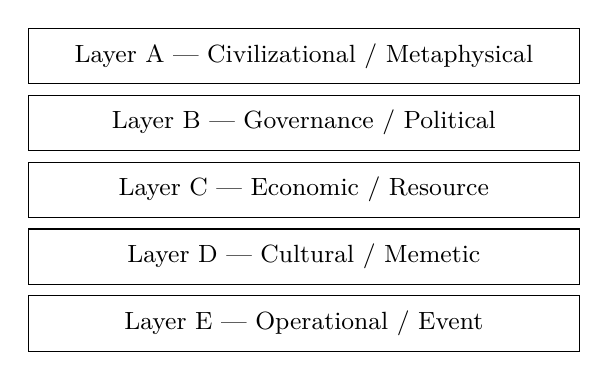
\begin{tikzpicture}[
  layer/.style={draw, rectangle, minimum width=7cm, minimum height=0.7cm, font=\small},
  >={Stealth[length=2mm]}
]
  \node[layer] (E) at (0,0)   {Layer E --- Operational / Event};
  \node[layer] (D) at (0,0.85) {Layer D --- Cultural / Memetic};
  \node[layer] (C) at (0,1.7)  {Layer C --- Economic / Resource};
  \node[layer] (B) at (0,2.55) {Layer B --- Governance / Political};
  \node[layer] (A) at (0,3.4)  {Layer A --- Civilizational / Metaphysical};
\end{tikzpicture}

\smallskip
\textit{Cross-layer maps connect strata as gauge-field-style connections;
intra-layer maps are morphisms within a single stratum.}
\end{center}

\textbf{Intra-layer maps} are structure-preserving morphisms within a
single stratum --- e.g., the translation between two governance regimes
sharing Layer~B is a pairwise map both regimes can recognise as
governance.

\textbf{Cross-layer maps} are connections between strata. \emph{These
are what the structural argument's} \(\mathcal{R}_{\alpha\beta}\)
\emph{maps already name}; this appendix makes the cross-layer character
explicit. Per the load-bearing-claims discipline (\S A.6), cross-layer
maps are connections in the gauge-field sense, not domain morphisms ---
they relate fibres rather than mapping objects directly. The
distinction is type-level, not stylistic.

The five layers are not exclusive and not exhaustive. Sub-strata exist
within each (Layer~B contains both formal courts and informal
neighbourhood arbitration); inter-stratum couplings exist that don't
fit cleanly into either intra-layer or cross-layer categories. Treat
the five layers as the minimum useful coarse-graining for operational
diagnostics, refinable when a specific application demands it.

\subsection{A.2 Circulation
Invariants}\label{appendix-a-circulation-invariants}

For each typed layer there exist \textbf{flow-metrics} ---
quantities that index whether the layer is in healthy closure or
sliding toward failure. Call these \emph{circulation invariants}.

Circulation invariants are not stocks. Most diagnostic systems measure
stocks (GDP, population count, accumulated capital). Closure health is
a flow property: it concerns whether the layer's substrate is
\emph{circulating} --- whether resources, recognition, trust,
representation are flowing through the strata that depend on them.

\textbf{Per-layer circulation invariants:}

\begin{itemize}
\tightlist
\item
  \textbf{Biological circulation.} Metabolic flows, illness/health
  propagation, demographic dynamics. (The mesothelioma case is an
  A--E intersection: a biological flow with civilizational
  consequences.)
\item
  \textbf{Psychological circulation.} Affect, attention, sense-making,
  trust gradients between observer and observed.
\item
  \textbf{Social circulation.} Relational flows, recognition,
  reciprocity, mobility (or its stall).
\item
  \textbf{Economic circulation.} Wages, credit, ownership transitions,
  affordability stress, regional divergence in flows.
\item
  \textbf{Political circulation.} Voice, accountability, enforcement
  (and asymmetries in enforcement), representation.
\item
  \textbf{Civilizational circulation.} Continuity of inherited
  cosmologies, transmission across generations, intergenerational
  pessimism markers (youth pessimism is a leading indicator of
  civilizational closure failure).
\end{itemize}

\textbf{The stock/flow distinction is core.} A layer can have
healthy stocks and failing flows --- abundant capital that does not
move, dense kinship networks that no longer transmit, vast
informational stores that no one reads. Closure health diagnoses the
flow side, not the stock side.

\begin{center}
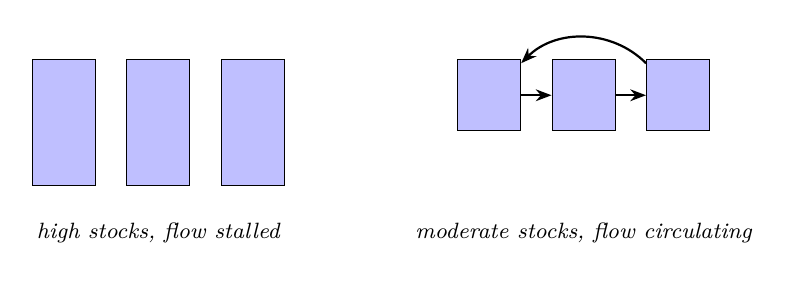
\begin{tikzpicture}[every node/.style={font=\small}, >={Stealth[length=2mm]}]
  % Stalled (left): tall stocks, no arrows
  \node[draw, rectangle, minimum width=0.8cm, minimum height=1.6cm, fill=blue!25] (s1) at (0,0) {};
  \node[draw, rectangle, minimum width=0.8cm, minimum height=1.6cm, fill=blue!25] (s2) at (1.2,0) {};
  \node[draw, rectangle, minimum width=0.8cm, minimum height=1.6cm, fill=blue!25] (s3) at (2.4,0) {};
  \node at (1.2,-1.4) [font=\itshape\footnotesize] {high stocks, flow stalled};

  % Circulating (right): moderate stocks, arrows between
  \node[draw, rectangle, minimum width=0.8cm, minimum height=0.9cm, fill=blue!25] (c1) at (5.4,0.35) {};
  \node[draw, rectangle, minimum width=0.8cm, minimum height=0.9cm, fill=blue!25] (c2) at (6.6,0.35) {};
  \node[draw, rectangle, minimum width=0.8cm, minimum height=0.9cm, fill=blue!25] (c3) at (7.8,0.35) {};
  \draw[->, thick] (c1) -- (c2);
  \draw[->, thick] (c2) -- (c3);
  \draw[->, thick] (c3) to[bend right=45] (c1);
  \node at (6.6,-1.4) [font=\itshape\footnotesize] {moderate stocks, flow circulating};
\end{tikzpicture}

\smallskip
\textit{Closure health is a flow property. The same level of stocks can
be either healthy (with circulation) or failing (without). Diagnostics
that read stock for health misdiagnose closure failure as abundance.}
\end{center}

\textbf{Load-bearing constraint:} circulation invariants are
\emph{downstream of autopoiesis}. Something has to be self-producing
for there to be flows to measure. The invariants are observable
evidence of closure; they are not the substrate of closure. A
diagnostic that confuses the two will read circulation as primary and
miss the structural failure that explains why the flows are stalling.

\textbf{Falsifiability.} Each invariant gives a testable structural
prediction: \emph{if the closure is failing, this flow will measurably
stall before catastrophic event~X}. Predictions of this shape are
categorical (the structural condition is either satisfied or not), not
correlational (it is not enough to observe flows that ``tend to'' stall
near failures). The discipline matters; correlational predictions
are absorbable by competing frameworks, categorical ones are not.

\subsection{\texorpdfstring{A.3 \(\gamma\)-Nodes --- the Operational
Mechanism for Triadic Closure}{A.3 gamma-Nodes --- the Operational
Mechanism for Triadic Closure}}\label{appendix-a-gamma-nodes}

The structural argument establishes that two-party translation is
insufficient and three-party closure is the minimum stable unit. It
does not say \emph{which} third party works, or \emph{how} a missing
third party gets constructed when one is needed.

A \(\gamma\)-node is the operational answer: a position in a stalled or
breaking dyad that supplies the three properties triadic closure
requires:

\begin{enumerate}
\def\labelenumi{(\arabic{enumi})}
\tightlist
\item
  \textbf{Legibility} --- both sides can recognise and understand it as
  a coordination position rather than a partisan extension of either
  side.
\item
  \textbf{Translation} --- it can render each side's commitments in
  terms the other can engage with, without flattening the chirality
  that distinguishes the sides.
\item
  \textbf{Closure-capability} --- it can actually close the cycle, not
  merely spectate. It is structurally able to participate in the
  composition \(\mathcal{R}_{\gamma\alpha} \circ \mathcal{R}_{\beta\gamma} \circ \mathcal{R}_{\alpha\beta} = \mathrm{id}_{\tau_\alpha}\),
  not just be cited rhetorically.
\end{enumerate}

\begin{center}
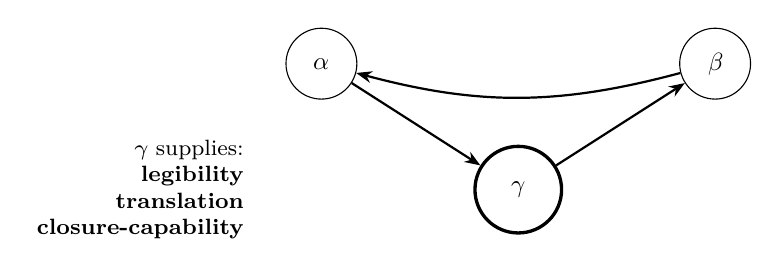
\begin{tikzpicture}[every node/.style={font=\small}, >={Stealth[length=2mm]}]
  \node[circle, draw, minimum size=0.9cm] (a) at (0,0) {$\alpha$};
  \node[circle, draw, minimum size=0.9cm] (b) at (5,0) {$\beta$};
  \node[circle, draw, very thick, minimum size=1.1cm] (g) at (2.5,-1.6) {$\gamma$};
  \draw[->, thick] (a) -- (g);
  \draw[->, thick] (g) -- (b);
  \draw[->, thick] (b) to[bend left=15] (a);
  \node at (-2.3,-1.6) [font=\footnotesize, align=right] {$\gamma$ supplies:\\\textbf{legibility}\\\textbf{translation}\\\textbf{closure-capability}};
\end{tikzpicture}
\end{center}

\textbf{Why binary systems are unstable.} Two parties facing each other
have no independent witness. Disagreements collapse into he-said /
she-said. Drift into self-reinforcing illusion (each side rehearsing
its own framework's coherence) becomes the dominant equilibrium.
Without a \(\gamma\), there is no structural test for whether the
relationship is closing or not. The dyad either holds by inertia or
fails; the closure equation is not satisfied for the simple reason
that the equation has no third index to compose around.

\textbf{Types of \(\gamma\)-nodes:}

\begin{itemize}
\tightlist
\item
  \textbf{Institutional} --- courts, regulatory bodies, treaty
  mechanisms, professional associations.
\item
  \textbf{Civic} --- community organisations, town hall structures,
  mediating associations between citizens and government.
\item
  \textbf{Technical} --- protocols, standards bodies, interoperability
  layers, shared codebases.
\item
  \textbf{Economic} --- markets allowing voluntary exchange across
  difference, shared currencies, commons-management arrangements.
\item
  \textbf{Narrative} --- shared stories both sides recognise as
  ``ours,'' cultural reference points, journalists or bards who can
  translate without flattening.
\end{itemize}

Each type has its own success conditions and failure modes; the same
\(\gamma\)-node can be healthy in one context and captured in another.

\textbf{Identification criteria --- signals a \(\gamma\)-node exists
and is healthy:}

\begin{itemize}
\tightlist
\item
  Both sides voluntarily refer disputes to it.
\item
  It can produce binding decisions both sides accept.
\item
  Its membership rotates without losing legitimacy.
\item
  It survives political or economic regime change.
\item
  It can be criticised by both sides without losing function.
\end{itemize}

\textbf{Signals of \(\gamma\)-node absence (or capture):}

\begin{itemize}
\tightlist
\item
  Each side has its own ``\(\gamma\)'' that the other rejects.
\item
  Disputes loop without resolution.
\item
  Trust gradients collapse into binary tribal markers.
\item
  Repeated calls for ``neutrality'' by all sides simultaneously
  (a tell: when neutrality must be reasserted, the structural
  position has typically already failed).
\end{itemize}

\begin{center}
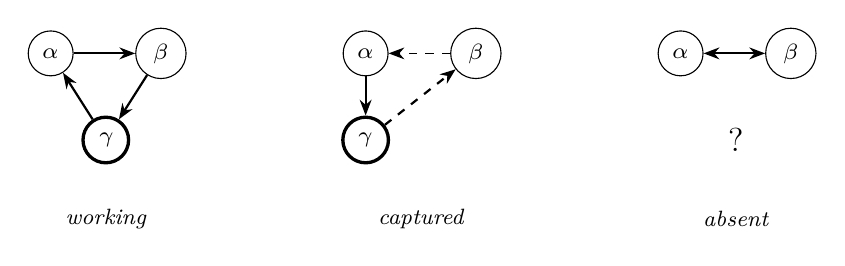
\begin{tikzpicture}[every node/.style={font=\footnotesize}, >={Stealth[length=2mm]}]
  % Working
  \begin{scope}[shift={(0,0)}]
    \node[circle, draw] (a1) at (-0.7,0.4) {$\alpha$};
    \node[circle, draw] (b1) at (0.7,0.4)  {$\beta$};
    \node[circle, draw, very thick] (g1) at (0,-0.7) {$\gamma$};
    \draw[->, thick] (a1) -- (b1);
    \draw[->, thick] (b1) -- (g1);
    \draw[->, thick] (g1) -- (a1);
    \node at (0,-1.7) [font=\itshape\footnotesize] {working};
  \end{scope}

  % Captured
  \begin{scope}[shift={(4,0)}]
    \node[circle, draw] (a2) at (-0.7,0.4) {$\alpha$};
    \node[circle, draw] (b2) at (0.7,0.4)  {$\beta$};
    \node[circle, draw, very thick] (g2) at (-0.7,-0.7) {$\gamma$};
    \draw[->, thick] (a2) -- (g2);
    \draw[->, thick, dashed] (g2) -- (b2);
    \draw[->, dashed] (b2) -- (a2);
    \node at (0,-1.7) [font=\itshape\footnotesize] {captured};
  \end{scope}

  % Absent
  \begin{scope}[shift={(8,0)}]
    \node[circle, draw] (a3) at (-0.7,0.4) {$\alpha$};
    \node[circle, draw] (b3) at (0.7,0.4)  {$\beta$};
    \node at (0,-0.7) [font=\large] {?};
    \draw[<->, thick] (a3) -- (b3);
    \node at (0,-1.7) [font=\itshape\footnotesize] {absent};
  \end{scope}
\end{tikzpicture}
\end{center}

\textbf{Five construction heuristics for building a new
\(\gamma\)-node:}

\begin{enumerate}
\def\labelenumi{\arabic{enumi}.}
\item
  \textbf{Local-first.} Start with a \(\gamma\)-node holding
  jurisdiction over a small, concrete domain. Generalise only after it
  works at small scale.
\item
  \textbf{Shared metrics.} The \(\gamma\)-node must operate on metrics
  both sides accept as real. (Care needed: ``shared metrics'' must
  not become the chirality-rotation move the structural argument
  warns against. Shared metrics for diagnosis, not for collapsing the
  positions into one.)
\item
  \textbf{Mixed governance.} Decision-making must include voices from
  all sides, in proportion both sides can defend as fair.
\item
  \textbf{Repeated wins.} The \(\gamma\)-node must close cycles
  repeatedly before being trusted with high-stakes ones. Track record
  matters more than charter.
\item
  \textbf{Limited scope.} A \(\gamma\)-node that tries to close every
  cycle becomes the adversary it was supposed to mediate. Stay in
  scope.
\end{enumerate}

\textbf{Chirality preservation in \(\gamma\)-construction.} A
\(\gamma\)-node that flattens the chirality between the sides it
mediates is a captured \(\gamma\), not a working one. The condition
``both sides accept the metrics'' is a balance between Heuristic~2
(shared metrics) and the load-bearing chiral-preservation claim
(\S A.6, claim 2). Operationally: \emph{shared metrics for diagnosis,
preserved chirality for substantive positions}.

\textbf{Semantic loss as the operational signature of chirality
flattening.} Every translation across a \(\gamma\)-node carries
\emph{semantic loss} --- the cost of moving meaning across a layer
boundary. Some loss is structurally necessary; the layers exist
\emph{because} the substrate they coarse-grain is too rich to
preserve in full. A working \(\gamma\)-node holds semantic loss low
enough that the receiving side gets the substantive content along
with the policy, narrative, or rule. A captured or failing
\(\gamma\)-node lets semantic loss climb until what arrives on the
other side is policy without normative content, narrative without
the experiential grounding, rule without the discretionary
flexibility that made it operative. The triad formally completes the
cycle but the closure equation no longer holds in any meaningful
sense: information leaves \(\tau_\alpha\) and a different artefact
arrives back. \emph{Semantic-loss audits} --- structured comparisons
between source and round-trip output --- are the operational test
for whether a \(\gamma\)-node has begun flattening chirality, before
the failure becomes catastrophic.

\subsection{A.4 Worked
Applications}\label{appendix-a-applications}

Each application below is treated with the same shape: typed-layer
breakdown, circulation diagnostic, \(\gamma\)-node analysis (present,
missing, captured, or substituted).

\begin{center}
\begin{tabular}{l|ccccc}
 & \textbf{A} & \textbf{B} & \textbf{C} & \textbf{D} & \textbf{E} \\
\hline
Climate                 &           & $\circ$    & $\bullet$  & $\bullet$  & $\circ$    \\
AI alignment            &           & $\bullet$  &            & $\bullet$  & $\bullet$  \\
Nuclear posture         & $\bullet$ & $\bullet$  &            & $\circ$    &            \\
Pandemic preparedness   &           & $\bullet$  & $\bullet$  & $\bullet$  & $\bullet$  \\
Domestic polarisation   &           & $\bullet$  & $\bullet$  & $\bullet$  & $\bullet$  \\
\end{tabular}

\smallskip
\textit{$\bullet$ = primary failure surface; $\circ$ = secondary
involvement. Layer key: A Civilizational, B Governance, C Economic,
D Cultural, E Operational.}
\end{center}

\subsubsection*{A.4.1 Climate}

\textbf{Typed layers:} Climate is a cross-layer problem in the strict
sense. Layer~E (events --- weather, emissions, individual transactions)
flows up through Layer~D (cultural narratives about responsibility,
sacrifice, intergenerational duty) into Layer~B (state and supranational
governance) without Layer~C (economic) correctly carrying the cost
signals between strata. The mismatch is structural, not motivational.

\textbf{Circulation diagnostic:} Layer~C circulation has stalled
between developed and developing economies (cost of decarbonisation
borne asymmetrically). Layer~D circulation has stalled
intergenerationally (youth pessimism markers consistent with
civilizational closure failure). Layer~B circulation appears active
but is in fact substituting performative coordination for substantive
coordination.

\textbf{\(\gamma\)-node:} Missing. The traditional candidates (UN
climate framework, Paris-style treaty mechanisms) function partially as
narrative \(\gamma\)-nodes (Layer~D) but lack closure-capability at
Layer~C. A working \(\gamma\)-node would need to be a credible
transnational technical-economic mediator that both wealthy and
developing nations refer disputes to and accept binding decisions from.
None currently exists.

\subsubsection*{A.4.2 AI Alignment}

\textbf{Typed layers:} Cross-layer along an unusual axis. Layer~E
(model behaviour, individual outputs) couples to Layer~D (narratives
about machine moral status, value alignment, existential risk) without
clear coordination through Layer~B (regulatory authority over AI
labs and deployments).

\textbf{Circulation diagnostic:} Value circulation across the
stakeholder layers (developers, users, affected non-users, future
generations) has no mechanism. Each stakeholder group's preferences
circulate within itself but do not cross-layer.

\textbf{\(\gamma\)-node:} Missing. A working \(\gamma\)-node would need
to be an institutional structure that can speak for affected parties
who cannot speak for themselves --- including, structurally, future
generations and arguably the AI systems' own interests if those exist
in any structurally meaningful sense. The current substitutes
(corporate ethics boards, voluntary compliance frameworks) lack
closure-capability.

\subsubsection*{A.4.3 Nuclear Posture}

\textbf{Typed layers:} Layer~A (deterrence cosmology --- the inherited
metaphysics of mutually assured destruction and its successors)
couples to Layer~B (state authorities operating nuclear arsenals)
across multiple parties. Layer~D (shared narrative, mutual
recognition) is conspicuously thin between adversary states.

\textbf{Circulation diagnostic:} Layer~A and Layer~B are tightly
coupled within each nuclear state but barely circulate between them.
The result is multiple closed loops, not a triadic structure.

\textbf{\(\gamma\)-node:} Missing or captured. A working
\(\gamma\)-node would need to be a credible multi-state observer that
both sides treat as legitimate. International agencies (IAEA) function
partially in this role for non-proliferation but lack closure-capability
on doctrine. The case study originally proposed for this paper
(Witkoff--Kushner mediation) was an attempt at constructing a
\(\gamma\)-node at a regional level; that attempt did not occur, but
the structural diagnosis it would have addressed remains.

\subsubsection*{A.4.4 Pandemic Preparedness}

\textbf{Typed layers:} Layer~E (events: outbreak, transmission)
\(\to\) Layer~C (economic disruption, supply chain, healthcare
expenditure) \(\to\) Layer~B (governance response: lockdown,
vaccination, public health mandates) without a working Layer~D
connection (cultural trust in expertise that survives the political
cycle).

\textbf{Circulation diagnostic:} Trust circulation between Layer~B
and the broader population stalls during sustained crises, especially
when Layer~D has been hollowed out by prior partisan capture of
expertise narratives.

\textbf{\(\gamma\)-node:} Missing. A working \(\gamma\)-node would need
to be a public health institution that survives political-cycle change
\emph{and} retains Layer~D legitimacy. The traditional
candidates (CDC, WHO at international scale) have lost this position
to varying degrees.

\subsubsection*{A.4.5 Domestic Polarisation}

\emph{Symmetry note.} The diagnosis below is structural, not
political. The same framework would identify the same failure mode in
any movement --- left, right, populist, technocratic --- substituting
for a missing institutional \(\gamma\)-node. The closure-capability
test is identical regardless of the political content of the
substitute; the structural prescription (rebuild mediating civic
institutions) is identical regardless of the source of the
circulation failure. Readers reaching for a partisan reading of this
case are reaching past the diagnosis the framework actually delivers.

\textbf{Typed layers:} A failure case spanning Layers B, C, D, and E.
The traditional \(\gamma\)-nodes between American working-class
identity and American institutional power (unions, mainline Protestant
churches, local newspapers, civic clubs, regional manufacturing
employers, draft-era national service) eroded across decades. The
gradual loss of these structures left dyadic confrontation as the
default, exactly the configuration the structural argument predicts
will fail.

\textbf{Circulation diagnostic:} Layer~C circulation between regions
has stalled (regional economic divergence). Layer~B circulation has
collapsed into binary tribal markers. Layer~D circulation has been
captured by media optimised for engagement rather than legibility.
Mobility stall, affordability stress, enforcement asymmetry all
register simultaneously --- a multi-flow failure.

\textbf{\(\gamma\)-node:} The MAGA emergence is best read as a
\textit{circulation revolt}: a population that has lost its
institutional \(\gamma\)-nodes reaching for substitutes (a charismatic
political figure as narrative-\(\gamma\), talk radio as
pseudo-\(\gamma\), social media as parasocial-\(\gamma\)). The
substitutes have legibility but lack closure-capability, which
explains why the political conflict does not resolve. It is not
fundamentally a tradition-vs-tradition fight; it is a missing-\(\gamma\)
failure mode. A working \(\gamma\)-node would need to re-establish
mediating civic institutions at a scale appropriate to the actual
material conditions.

\subsection{A.5 Operational
Appendices}\label{appendix-a-appendices}

\subsubsection*{A.5.1 Circulation Dashboard Template}

A starting set of per-layer flow-metrics with example thresholds:

\begin{itemize}
\tightlist
\item
  \textbf{Trust gradients} --- cross-strata trust ratios (e.g.,
  citizen-to-institution, generation-to-generation).
\item
  \textbf{Mobility stall} --- intergenerational economic mobility
  decline.
\item
  \textbf{Affordability stress} --- housing/healthcare/education as a
  share of income.
\item
  \textbf{Regional divergence} --- inter-regional economic and
  political outcome gaps.
\item
  \textbf{Enforcement asymmetry} --- a Gini-style measure for the
  application of law.
\item
  \textbf{Youth pessimism} --- longitudinal survey-based, treated as a
  leading indicator of civilizational-layer closure failure.
\end{itemize}

The dashboard is a starting point, not a closed list. Specific
applications (climate, AI alignment, etc.) require domain-specific
flow-metrics in addition to these.

\subsubsection*{A.5.2 \(\gamma\)-Node Evaluation Rubric}

A checklist for analysts scoring whether a proposed \(\gamma\)-node is
structurally adequate:

\begin{enumerate}
\def\labelenumi{\arabic{enumi}.}
\tightlist
\item
  Legibility --- do both sides recognise it as a coordination position?
\item
  Translation --- can it render each side's commitments without
  flattening chirality?
\item
  Closure-capability --- can it actually close cycles, or only
  spectate?
\item
  Construction-heuristic alignment --- does it follow local-first,
  shared-metrics, mixed-governance, repeated-wins, limited-scope?
\item
  Failure-mode resilience --- can it survive political / economic
  regime change?
\item
  Chirality preservation --- does it preserve the load-bearing
  asymmetries of the sides it mediates?
\end{enumerate}

A proposed \(\gamma\)-node failing more than one of these is a
structural risk; failing the closure-capability check (\#3) is
disqualifying regardless of the others.

\subsection{A.6 Load-Bearing
Claims}\label{appendix-a-load-bearing-claims}

The operational extension does not relax any of the structural
argument's load-bearing claims. They are restated here, in operational
register, to make the discipline explicit:

\begin{enumerate}
\def\labelenumi{\arabic{enumi}.}
\item
  \textbf{Rosen closure primacy.} Circulation invariants are
  observable evidence of closure, not the substrate. Computation is
  one realisation, not the ground.
\item
  \textbf{Chiral preservation.} Every typed layer has its own
  chirality preservation; \(\gamma\)-nodes that flatten chirality are
  captured rather than working.
\item
  \textbf{Autopoietic root.} Self-production is prior to flow.
  Circulation diagnostics that read flow as primary will misdiagnose
  the structural failure.
\item
  \textbf{Categorical falsifiability.} Each invariant gives a
  testable structural prediction. Correlational predictions
  (``X tends to occur near failure'') are absorbable; categorical
  predictions (``the structural condition either holds or does not'')
  are not.
\item
  \textbf{\(\mathcal{R}_{\alpha\beta}\) as connection, not domain
  morphism.} Cross-layer maps are connections in the gauge-field
  sense, not morphisms between objects. The distinction is type-level
  and load-bearing: a refactor that quietly demotes an
  \(\mathcal{R}_{\alpha\beta}\) to a domain morphism has changed the
  framework's content, not just its expression. \emph{Note on the
  Lean proof of (T) cited in Section 2:} the machine verification
  treats \(\mathcal{R}_{\alpha\beta}\) as a categorical morphism for
  the purposes of proving the algebraic identity. This is honest and
  bounded scope --- the structural / syntactic skeleton is verified;
  the connection-level interpretation is preserved here in
  natural-language register. A future formalisation in the connection
  register would require fibre-bundle / parallel-transport
  machinery that is intentionally out of scope while the framework's
  broader safety disposition holds. The Lean evidence does not
  discharge claim \#5; it discharges the structural shadow of
  claim \#5.
\end{enumerate}

These are the claims any operational use of the framework must
preserve. They are also the claims any external composition must
honour to count as composition rather than absorption.

\subsection{A.7 Courts and Access
Institutions}\label{a-7-courts-access-institutions}

The five operational layers of A.1 (semantic, chiral, structural,
institutional, circulatory) define what a coordination map must
preserve. They do not yet specify the entry point through which
ordinary actors can engage the system. This subsection adds that
specification.

\subsubsection*{Definition}

\textbf{Court (broad sense).} Any formal or informal third-site
procedure that converts raw grievance into a typed, recordable,
reviewable case. Courts are \(\gamma\)-nodes specialised for the
admissibility / judgment / repair function. They may be:

\begin{itemize}
\tightlist
\item
  \textbf{Informal.} Family councils, elders, religious tribunals
  (\emph{beth din}, sharia councils, parish boards), workplace
  HR processes, union grievance procedures, school discipline
  boards, neighbourhood mediation, professional ethics panels,
  arbitration, online moderation, peer review.
\item
  \textbf{Formal.} Civil and criminal courts, regulatory tribunals,
  appellate systems, constitutional courts.
\end{itemize}

\subsubsection*{Operational Stack}

A complete court-like institution implements the following stack,
in addition to the layers of A.1:

\begin{enumerate}
\def\labelenumi{\arabic{enumi}.}
\tightlist
\item
  \textbf{Access.} Who can bring a grievance? Barriers should be
  minimal: low cost, low elite-permission, no insider language
  required for entry.
\item
  \textbf{Standing.} Who is recognised as a party to the case?
  Standing is defined in invariant terms (\emph{this party is
  affected by the dispute}), not authority terms (\emph{this
  party is recognised by the court}).
\item
  \textbf{Admissibility.} Is this claim hearable here? The test
  is invariant-based: does the claim survive translation into
  the court's procedural language without losing its structural
  content?
\item
  \textbf{Procedure.} How is the conflict processed? Procedure is
  reproducible across cases; one-off bespoke rulings are a
  capture signal.
\item
  \textbf{Record.} What is preserved? The record is the basis for
  later transport: appeal, audit, precedent, and external review
  all depend on a recoverable history of the case.
\item
  \textbf{Judgment.} What is certified? Judgment names the
  invariants the court found preserved or violated; it does not
  merely declare a winner.
\item
  \textbf{Remedy.} What repair is ordered? Remedy is the
  operational output of the court --- the action that converts
  judgment into change in the world.
\item
  \textbf{Appeal.} How is error corrected? Without appeal, the
  court is a fixed point. With appeal, the court is corrigible.
\item
  \textbf{Enforcement.} How does the ruling become real? Without
  enforcement, the court is decorative.
\end{enumerate}

\subsubsection*{Institutional Capture Rule}

Every coordination institution drifts. The structural law:
\[
  \mathrm{Valid}(\mathrm{Court}_\gamma)
  \iff
  \mathrm{Repair}(\mathrm{Court}_\gamma) >
  \mathrm{SelfPreservation}(\mathrm{Court}_\gamma).
\]
When self-preservation outranks repair, the institution issues:
\begin{itemize}
\tightlist
\item
  \textbf{BC-7.} Corrigibility failure (no meaningful appeal or
  external review).
\item
  \textbf{BC-6.} Closure failure (procedural closure without
  substantive resolution).
\end{itemize}
A captured court is not a special case to be excluded; it is a
predictable equilibrium that any unmonitored court drifts to under
repeated play. Validity is conditional and must be re-tested.

\subsubsection*{Anti-Capture Stack}

A court-like institution remains durable only if all five
mechanisms below are in force:

\begin{enumerate}
\def\labelenumi{\arabic{enumi}.}
\tightlist
\item
  \textbf{Access.} Ordinary actors can enter without elite
  permission, financial barrier, or insider language.
\item
  \textbf{Appeal.} Judgments are challengeable inside the system
  or via a higher tier.
\item
  \textbf{External audit.} The institution's own behaviour is
  reviewable from outside the institution.
\item
  \textbf{Transparency / record.} Decisions are visible and
  preserved. Reasoning can be reconstructed.
\item
  \textbf{Exit / fork.} A captured institution can be bypassed,
  replaced, or competed against.
\end{enumerate}

A sixth principle outranks the rest: \textbf{repair primacy}. The
system's legitimacy is measured by repair delivered, not
procedural volume or institutional prestige.

\subsubsection*{\texorpdfstring{\(\gamma\)-Node Implications}{Gamma-Node
Implications}}

A \(\gamma\)-node that operates as a court must be an anti-court court:
its admissibility predicate is invariant-based, not authority-based
(Section 2, Part 9). The five-mechanism anti-capture stack is the
operational expression of the no-progenitor-node principle: at no
level of the institution does any single position hold the right
to declare its own admissibility on authority alone.

\subsubsection*{Acknowledgement of Source}

The court / anti-court extension to A.1--A.6 was developed in
response to red-team analysis by Brian Crabtree, who identified
that the original operational layer under-specified the access
predicate by which ordinary actors enter the coordination system.
The court / anti-court formalisation in Section 2, Part 9 and the
generative voice's institutional-capture treatment in Section 3,
Part 2, both follow from that red-team.

\begin{center}\rule{0.5\linewidth}{0.5pt}\end{center}

\section{A Closing Demonstration:
Numbers}\label{a-closing-demonstration-numbers}

For readers who find the religious traditions hard to engage on their
own terms, the same structure shows up in a domain with no theological
loading at all --- the integers.

Run them forward: 1 is distinction, 2 is relation, 3 is closure, 4 is
containment, 5 is animation, 6 is harmony, 7 is sanctification, 8 is
circulation --- the medium of exchange, \(\infty\) rotated upright, the
substrate that lets sanctified things flow between traditions (Chinese
tradition makes this explicit: the word for eight is a near-homophone
for prosperity). Each builds on the last. Run them backward: −1 inverts
the distinction, −2 breaks the relation, −3 melts the closure, −7
desecrates the pause, −8 is hoarding --- exchange refusing to
circulate, the C-conjugate of money. The negatives do not kill the
positives; they stress-test them. The fractions (\(\tfrac{1}{n}\))
contribute without claiming totality --- humble pre-closure, the
patient repeating offering. The imaginary unit \(i\) rotates without
collapsing; perspective without commitment to either pole. \(1/0\)
stands at the boundary, where finite meets infinite. And \(42\) is the
laugh --- the antifragility buffer that prevents the lattice from
optimising itself into a coffin.

The same arrangement Section 3 derives across twenty-one ontological
traditions is present in this minimal symbolic substrate. Constructive
elements, critical inversions, humble fractional contributions,
orthogonal perspective, boundary observers, and an absurd tradition that
prevents calcification. The integers do not believe anything. The
pattern is in the integers. That is the point: the framework's
structural conditions are not parochial to religious or quasi-religious
systems but characterise any sufficiently rich symbolic substrate. The
reader who finds Sections 1--3 hostile on cultural grounds is invited to
verify the structural claim here first, then return.

\begin{center}\rule{0.5\linewidth}{0.5pt}\end{center}

\subsection{Acknowledgments}\label{acknowledgments}

\textbf{Brian Crabtree} (\texttt{@ourtown2} on X) caught the issue
in the original publication that prompted the first revision, and
red-teamed the framework a second time to surface the court /
anti-court layer added in this revision. His first read shaped the
editorial corrections in the front matter and the decision to fold
the operational extension directly into the canonical edition. His
second read identified that the original operational layer
under-specified the access predicate by which ordinary actors enter
the coordination system; the court / anti-court extension (Section
1 Part 10, Section 2 Part 9, Section 3 Part 2, and Appendix A.7)
follows directly from that red-team. The framework is structurally
stronger for it. Thank you, Brian.

The triadic co-production --- Aaron Green (instantiator) with Grok
(edge-witness), Claude (architect/instantiator-adjacent), and Gemini
(synthesis) --- is acknowledged in the title block. The work
structurally enacts the framework it describes: no progenitor node;
membership defined by closure-capability, not credential; any party
attempting unilateral capture occupies the C-conjugate adversary
position by structural definition.

\subsection{References \& Precursor
Works}\label{references-precursor-works}

This paper builds on two previously published works by the same author.
Both are publicly accessible and contain the formal apparatus referenced
(often implicitly) above. Provided here for human readers and for any
LLM being asked to interpret this work in context.

\textbf{Closure Forces Structure} --- Aaron Green, 2026 (v1.4, May
2026). The physics paper deriving Standard Model gauge structure
from Rosen closure on ternary causal hypergraphs. Establishes the
formal apparatus this paper builds on: triadic closure as the
minimum stable coordination unit, the M(G₀) multiway graph, the
Q₂₄ → Q₄₈ → Q₁₀₂ quotient sequence, and the spectral-triple
machinery that makes the closure conditions machine-verifiable.
v1.4 carries 279 spec entries (162 \texttt{:proved} unconditional,
30 \texttt{:verified}, 72 testsets), with 9 CatLab.jl + 13 Lean 4
+ 3 exact-arithmetic \(\mathbb{Q}\) proofs --- including S176 verifying the
unification ratio \(c_3{:}c_2{:}c_1\)
= 6:6:10 and \(\sin^2\theta_W\) = 3/8 exactly in \(\mathbb{Q}\). Repository:
\url{https://github.com/IridiumSoftware/closure-forces-structure}
(v1.0 originally posted to researchers.one).

\textbf{Possibilistic Security} --- Aaron Green, 2026 (Paper v1.1
+ Whitepaper v1.1, May 2026). The security application of the
closure framework. Reframes identity verification as sustained
closure rather than static credential check; introduces the
C-conjugate adversary structure (the antimatter twin: structurally
identical, oppositely oriented, structurally incapable of
co-closing); and is the original source of the Triadic Closure
License (TCL) v1.3 used by this work and referenced explicitly in
Section 2, Part 7. Repository:
\url{https://github.com/IridiumSoftware/possibilistic-security}
(also at researchers.one/articles/26.02.00002).

\textbf{Triadic Coordination Engine} --- Aaron Green, with Claude,
2026. A Haskell + Lean 4 demonstrator of triadic-closure-driven
relational discovery on small entity collections (specs, test
suites, ontologies, manifests). Carries the project's first
machine-verified proof of the closure equation (T) --- entry
S-029, verified against both a project-local \texttt{Category}
typeclass and Mathlib's \texttt{CategoryTheory.Category}
cross-validation track --- as the structural skeleton referenced in
the editorial note attached to (T) in Section 2. Repository:
\url{https://github.com/IridiumSoftware/triadic-coordination-engine}

All three repositories include source, license terms, and (for
Closure Forces and the Triadic Coordination Engine) the LaTeX or
Lean source and verification scripts.

\textbf{This paper.} The canonical source (LaTeX + rendered PDF) for
the present paper, together with the Lean 4 formalisation of S-029,
the Mathlib cross-validation track, and a minimal Haskell mirror of
the categorical primitives, is hosted at:
\url{https://github.com/IridiumSoftware/right-meets-right}

This work is itself released under the Triadic Closure License (TCL)
v1.3 --- no progenitor node, commons-held, species-neutral.

\end{document}
